\documentclass[a4paper, 14pt]{book}

%%%%%%%%%%%%%%%%%%%%%%%%%%%%%%%%%%%%%%%%%%%%%%%%%%%%%%%%
% packages
%%%%%%%%%%%%%%%%%%%%%%%%%%%%%%%%%%%%%%%%%%%%%%%%%%%%%%%%
\usepackage{xeCJK}
\usepackage{amsmath, amsthm, amscd, amssymb}
\usepackage{graphicx}
\usepackage{mathrsfs}
\usepackage{mathtools}
% \usepackage{citesort}
% \usepackage[numbers, sort&compress]{natbib}
\usepackage{anysize}
\marginsize{3cm}{3cm}{2.9cm}{2.8cm} \baselineskip 22pt
\usepackage[sf]{titlesec}
\usepackage{fancyhdr}
\usepackage{graphics}
\usepackage{graphicx}
\usepackage{subfigure}
% \usepackage{caption}
% \usepackage{ccaption}
\usepackage{tabularx}
\usepackage{multirow}
\usepackage{multicol}
% \usepackage{longtable}
% \usepackage{slashbox}
% \usepackage{supertabular}
\usepackage{float}
% \usepackage{diagbox}
% \usepackage{booktabs}
% \usepackage{cite}
\usepackage{bm}
\usepackage{arydshln}
% \usepackage{setspace}
\usepackage{boxedminipage}

\usepackage[ruled,linesnumbered,algosection,nofillcomment]{algorithm2e}
\renewcommand*{\algorithmcfname}{算法}
\renewcommand*{\algorithmautorefname}{算法}

\makeatletter
\renewcommand{\Indentp}[1]{%
  \advance\leftskip by #1
  \advance\skiptext by -#1
  \advance\skiprule by #1}%
\renewcommand{\Indp}{\algocf@adjustskipindent\Indentp{\algoskipindent}}
\renewcommand{\Indpp}{\Indentp{0.5em}}%
\renewcommand{\Indm}{\algocf@adjustskipindent\Indentp{-\algoskipindent}}
\renewcommand{\Indmm}{\Indentp{-0.5em}}%
\makeatother

\newcommand\mycommfont[1]{\footnotesize\ttfamily\textcolor{blue}{#1}}
\SetCommentSty{mycommfont}

\DontPrintSemicolon

\usepackage{tikz}
\usetikzlibrary{trees,arrows.meta,decorations.pathmorphing,decorations.pathreplacing,shapes,shapes.geometric,backgrounds,positioning,calc,tikzmark,external}

% 参考文献工具,加载biblatex宏包,
% 其后端backend使用biber,%标注(引用)样式citestyle,
% 著录样式 bibstyle都采用gb7714-2015样式,
% 两者相同时可以合并为一个选项style
% https://ctan.org/pkg/biblatex-gb7714-2015?lang=en
% https://www.overleaf.com/learn/latex/Articles/Getting_started_with_BibLaTeX
\usepackage[backend=biber,style=gb7714-2015]{biblatex}
\addbibresource[location=local]{references.bib}


%%%%%%%%%%%%%%%%%%%%%%%%%%%%%%%%%%%%%%%%%%%%%%%%%%%%%%%%
% Chinese fonts
%%%%%%%%%%%%%%%%%%%%%%%%%%%%%%%%%%%%%%%%%%%%%%%%%%%%%%%%

\setCJKmainfont[Path = fonts/, BoldFont = simhei.ttf]{simsun.ttc}
\setCJKsansfont[Path = fonts/, BoldFont = simhei.ttf]{simsun.ttc}
\setCJKmonofont[Path = fonts/, BoldFont = simhei.ttf]{simsun.ttc}

\newCJKfontfamily\kaishu[Path=fonts/]{simkai.ttf}
\newCJKfontfamily\songti[Path=fonts/]{simsun.ttf}
\newCJKfontfamily\heiti[Path=fonts/]{simhei.ttf}
\newCJKfontfamily\fangsong[Path=fonts/]{simfang.ttf}

%%%%%%%%%%%%%%%%%%%%%%%%%%%%%%%%%%%%%%%%%%%%%%%%%%%%%%%%
% miscelaneous settings
%%%%%%%%%%%%%%%%%%%%%%%%%%%%%%%%%%%%%%%%%%%%%%%%%%%%%%%%

% \numberwithin{algorithm}{section}%让算法按节编号!
% \floatname{algorithm}{算法}%将Algorithm替换为‘算法’

\newcommand{\citeu}[1]{$^{\mbox{\protect \scriptsize \cite{#1}}}$}
\newcommand{\eqabove}[1]{\stackrel{\mathclap{\normalfont\mbox{#1}}}{=}}
\newcommand{\neqabove}[1]{\stackrel{\mathclap{\normalfont\mbox{#1}}}{\neq}}

\newcommand{\p}{\partial}
%\newtheorem{exam}{\hei 算例}[chapter]
\newcommand\CJKprechaptername{第}
\newcommand\CJKchaptername{章}
\newcommand\CJKthechapter{\CJKnumber{\@arabic\c@chapter}}
\renewcommand{\tablename}{\kaishu 表}
\renewcommand{\figurename}{\kaishu 图}

\def\Def{~\overset{def}{=}~}  %def
\setlength{\unitlength}{1.2cm} %

\DeclareMathOperator*{\argmax}{arg\,max}
\DeclareMathOperator*{\argmin}{arg\,min}
\DeclareMathOperator*{\expectation}{\mathbb{E}}
\DeclareMathOperator*{\minimize}{minimize}

\newcommand{\R}{\mathbb{R}}

\renewcommand\arraystretch{1.2}

%===================== 重定义字体、字号命令 =============================%
\newCJKfontfamily\simfang{simfang.ttf}[Extension = .ttf, Path=fonts/]
\newCJKfontfamily\simhei{simhei.ttf}[Extension = .ttf, Path=fonts/]
\newCJKfontfamily\simkai{simkai.ttf}[Extension = .ttf, Path=fonts/]
\newCJKfontfamily\simsun{simsun.ttc}[Extension = .ttc, Path=fonts/]

\newcommand{\song}{\simsun}     % 宋体   (Windows自带simsun.ttf)
\newcommand{\fs}{\simfang}      % 仿宋体 (Windows自带simfs.ttf)
\newcommand{\kai}{\simkai}      % 楷体   (Windows自带simkai.ttf)
\newcommand{\hei}{\simhei}      % 黑体   (Windows自带simhei.ttf)
% \newcommand{\li}{\CJKfamily{li}}        % 隶书   (Windows自带simli.ttf)
% \newcommand{\you}{\CJKfamily{you}}      % 幼圆   (Windows自带simyou.ttf)
\newcommand{\chuhao}{\fontsize{42pt}{\baselineskip}\selectfont}           % 字号设置
\newcommand{\xiaochuhao}{\fontsize{36pt}{\baselineskip}\selectfont}       % 字号设置
\newcommand{\yihao}{\fontsize{28pt}{\baselineskip}\selectfont}            % 字号设置
\newcommand{\erhao}{\fontsize{22pt}{\baselineskip}\selectfont}            % 字号设置
\newcommand{\xiaoerhao}{\fontsize{18pt}{\baselineskip}\selectfont}        % 字号设置
\newcommand{\sanhao}{\fontsize{15.75pt}{\baselineskip}\selectfont}        % 字号设置
\newcommand{\sihao}{\fontsize{14pt}{\baselineskip}\selectfont}            % 字号设置
%\newcommand{\xiaosihao}{\fontsize{12pt}{20pt}\selectfont}                % 字号设置
\newcommand{\xiaosihao}{\fontsize{12pt}{14pt}\selectfont}                 % 字号设置
\newcommand{\wuhao}{\fontsize{10.5pt}{12.6pt}\selectfont}                 % 字号设置
\newcommand{\xiaowuhao}{\fontsize{9pt}{11pt}{\baselineskip}\selectfont}   % 字号设置
\newcommand{\liuhao}{\fontsize{7.875pt}{\baselineskip}\selectfont}        % 字号设置
\newcommand{\qihao}{\fontsize{5.25pt}{\baselineskip}\selectfont}          % 字号设置
%\iffalse

\makeatletter

%%%%%%%%%%%%%%%%%%%%%%%%%%%%%%%%%%%%%将目录中的第一章改成第1 章%%%%%%%%%%%%%%%%%%%%%%%%%%%%%%%%%%%%

\renewcommand{\chaptername}{第~\@arabic\c@chapter~章}
\renewcommand{\@makechapterhead}[1]{%
   \vspace*{-\baselineskip}%
   {\normalfont \flushleft\Large\bfseries%
   \chaptername \quad #1 \par\nobreak%
   \vspace{1.5\baselineskip}
   }}
\renewcommand{\@makeschapterhead}[1]{%
   \vspace*{-\baselineskip}%
   {\normalfont \flushleft\Large\bfseries #1 \par\nobreak%
   \vspace{1.5\baselineskip}
   }}

\def\@chapter[#1]#2{\ifnum \c@secnumdepth >\m@ne
                        \if@mainmatter
                          \refstepcounter{chapter}%
                          \typeout{第~\thechapter~章}%
                          \addcontentsline{toc}{chapter}%
                                    {\protect\numberline{}%
                                     第~\expandafter\noexpand\thechapter~ 章\hspace{0.8em}#1}%
                        \else
                          \addcontentsline{toc}{chapter}{#1}%
                        \fi
                     \else
                       \addcontentsline{toc}{chapter}{#1}%
                     \fi
                     \chaptermark{#1}%
                     \addtocontents{lof}{\protect\addvspace{10\p@}}%
                     \addtocontents{lot}{\protect\addvspace{10\p@}}%
                     \if@twocolumn
                       \@topnewpage[\@makechapterhead{#2}]%
                     \else
                       \@makechapterhead{#2}%
                       \@afterheading
                     \fi}

\makeatother

%画两条页眉线
%\pagestyle{plain}
 \pagestyle{fancy}
\newcommand{\makeheadrule}{%
    \makebox[0pt][l]{\rule[.7\baselineskip]{\headwidth}{0.5pt}}%
    \rule[.6\baselineskip]{\headwidth}{0.5pt}\vskip-.8\baselineskip}

\makeatletter
\renewcommand{\headrule}{%
    {\if@fancyplain\let\headrulewidth\plainheadrulewidth\fi
     \makeheadrule}}

%定义普通页眉
\fancyhf{}
\renewcommand{\chaptermark}[1]{\markboth{第\thechapter 章\ #1}{}}
\fancyhead[CO]{\song \leftmark}
\fancyhead[CE]{\song 北京航空航天大学博士后出站报告}
\fancyfoot[CE, CO]{\thepage}

%定义章首页的页眉和页脚.
\fancypagestyle{plain}{%
\fancyhead{} % clear all header fields
\fancyhead[CO]{\song \leftmark}
\fancyhead[CE]{\song 北京航空航天大学博士后研究工作报告}
\fancyfoot[CE, CO]{\thepage}}

%定义标题格式
\titleformat{\chapter}
   % {\normalfont\bfseries\huge\filcenter\CJKfamily{hei}}
    {\normalfont\LARGE\filcenter\rm}
    %{\huge{\chaptertitlename}}
    %{第~\CJKnumber{\thechapter}~章}
    {\bf 第\,{\thechapter}\,章}
    {18pt}{\rm}
\titlespacing{\chapter}{0pt}{-3ex  plus .1ex minus .2ex}{1.5ex plus .1ex minus .2ex}

\titleformat{\section}[hang]{\Large\bf}% add \bfseries if you want to use bold fonts
    {\Large \ \thesection}{1em}{}{}
\titlespacing{\section}%
    {0pt}{1.5ex plus .1ex minus .2ex}{\wordsep}%{1ex plus .1ex minus .2ex}

\titleformat{\subsection}[hang]{\large\bf}
    {\large\ \thesubsection}{1em}{}{}
\titlespacing{\subsection}%
    {0pt}{1.5ex plus .1ex minus .2ex}{\wordsep}

\raggedbottom
\parskip 0.1cm
\parindent 0.8cm

\numberwithin{equation}{section}
\newtheorem{theorem}{{\heiti 定理}}[section]
\newtheorem{definition}{{\heiti 定义}}[section]
\newtheorem{lemma}{{\heiti 引理}}[section]
\newtheorem{corollary}{{\heiti 推论}}[section]
\newtheorem{property}{{\heiti 性质}}[section]
\newtheorem{prop}{{\heiti 命题}}[section]
\newtheorem{assu}{{\heiti 假设}}[section]
\newtheorem{Proof}{{\heiti 证明}}[section]
\newtheorem{rem}{{\heiti 注记}}[section]
\newtheorem{con}{{\heiti 条件}}[section]
\newtheorem{example}{{\heiti 例}}[section]

\renewcommand*{\proofname}{证明}

\newcommand{\nc}{\newcommand}
%定义特殊短语
\newcommand{\tbc}{\red{TO BE CONTINUED...}}
\newcommand{\opp}{\red{OPEN PROBLEMS}.~}
%定义颜色
\newcommand{\red}{\textcolor{red}}
% open questions
\newcommand{\blue}{\textcolor{blue}}
% suspicious result or derivation
\newcommand{\green}{\textcolor{green}}
\newcommand{\white}{\textcolor{white}}

%定义空心大写字母
\nc{\bbA}{\mathbb{A}} \nc{\bbB}{\mathbb{B}} \nc{\bbC}{\mathbb{C}}
\nc{\bbD}{\mathbb{D}} \nc{\bbE}{\mathbb{E}} \nc{\bbF}{\mathbb{F}}
\nc{\bbG}{\mathbb{G}} \nc{\bbH}{\mathbb{H}} \nc{\bbI}{\mathbb{I}}
\nc{\bbJ}{\mathbb{J}} \nc{\bbK}{\mathbb{K}} \nc{\bbL}{\mathbb{L}}
\nc{\bbM}{\mathbb{M}} \nc{\bbN}{\mathbb{N}} \nc{\bbO}{\mathbb{O}}
\nc{\bbP}{\mathbb{P}} \nc{\bbQ}{\mathbb{Q}} \nc{\bbR}{\mathbb{R}}
\nc{\bbS}{\mathbb{S}} \nc{\bbT}{\mathbb{T}} \nc{\bbU}{\mathbb{U}}
\nc{\bbV}{\mathbb{V}} \nc{\bbW}{\mathbb{W}} \nc{\bbX}{\mathbb{X}}
\nc{\bbZ}{\mathbb{Z}}
 
 %定义特殊符号
\newcommand{\bra}[1]{\langle#1|}
\newcommand{\ket}[1]{|#1\rangle}
\newcommand{\proj}[1]{| #1\rangle\!\langle #1 |}
\newcommand{\ketbra}[2]{|#1\rangle\!\langle#2|}
\newcommand{\braket}[2]{\langle#1|#2\rangle}
\newcommand{\wetw}[2]{|#1\rangle\wedge|#2\rangle}
\newcommand{\weth}[3]{|#1\rangle\wedge|#2\rangle\wedge|#3\rangle}
\newcommand{\wefo}[4]{|#1\rangle\wedge|#2\rangle\wedge|#3\rangle\wedge|#4\rangle}
\newcommand{\norm}[1]{\lVert#1\rVert}
\newcommand{\abs}[1]{|#1|}
%定义特殊运算符
\def\xr{X_\r}
\def\xrg{X_{\r^\G}}
\def\axr{\abs{X_\r}}
\def\axrg{\abs{X_{\r^\G}}}


\def\locc{\mathop{\rm LOCC}}
\def\lu{\mathop{\rm LU}}
\def\max{\mathop{\rm max}}
\def\min{\mathop{\rm min}}
\def\mspec{\mathop{\rm mspec}}
\def\oghz{\mathop{\overline{\ghz}}}
\def\per{\mathop{\rm per}}
\def\ppt{\mathop{\rm PPT}}
\def\pr{\mathop{\rm pr}}
%\bQ, \bR, \bZ denotes the set of rational, real and integer numbers.
\newcommand{\pp}[2]{{\partial #1\over\partial #2}}

\nc{\cA}{{\cal A}} \nc{\cB}{{\cal B}} \nc{\cC}{{\cal C}}
\nc{\cD}{{\cal D}} \nc{\cE}{{\cal E}} \nc{\cF}{{\cal F}}
\nc{\cG}{{\cal G}} \nc{\cH}{{\cal H}} \nc{\cI}{{\cal I}}
\nc{\cJ}{{\cal J}} \nc{\cK}{{\cal K}} \nc{\cL}{{\cal L}}
\nc{\cM}{{\cal M}} \nc{\cN}{{\cal N}} \nc{\cO}{{\cal O}}
\nc{\cP}{{\cal P}} \nc{\cQ}{{\cal Q}} \nc{\cR}{{\cal R}}
\nc{\cS}{{\cal S}} \nc{\cT}{{\cal T}} \nc{\cU}{{\cal U}}
\nc{\cV}{{\cal V}} \nc{\cW}{{\cal W}} \nc{\cX}{{\cal X}}
\nc{\cZ}{{\cal Z}}

%符号
\def\ra{\rightarrow}
\def\Ra{\Rightarrow}
\def\su{\subset}
\def\sue{\subseteq}
\def\sm{\setminus}
\def\we{\wedge}
\def\Ps{\Psi}
\def\Ph{\Phi}


\def\diag{\mathop{\rm diag}}
\def\dim{\mathop{\rm Dim}}
\def\epr{\mathop{\rm EPR}}
\def\ev{\mathop{\rm EV}}
\def\tr{\mathop{\rm Tr}}
\def\lin{\mathop{\rm span}}
\def\rank{\mathop{\rm rank}}

\def\ba{\begin{array}}
	\def\ea{\end{array}}
\def\be{\begin{equation}}
\def\ee{\end{equation}}
\def\bg{\begin{aligned}}
	\def\eg{\end{aligned}}





\renewcommand{\theequation}{\thesection.\arabic{equation}}
\catcode`@=11 \@addtoreset{equation}{section} \catcode`@=12

 \allowdisplaybreaks
%\setlength{\topskip}{0.3in}   %%%%%%表示正文和页眉的间距
%\baselineskip 24pt            %%%%%%表示正文行距
\makeatletter
\renewenvironment{thebibliography}[1]
%org     {\chapter*{\bibname
%org    \@mkboth{\MakeUppercase\bibname}{\MakeUppercase\bibname}}%
     {\def\chaptername{}\chapter*{\bibname\@mkboth{\MakeUppercase\bibname}{\MakeUppercase\bibname}}%                            !!!
      \list{\@biblabel{\@arabic\c@enumiv}}%
           {\settowidth\labelwidth{\@biblabel{#1}}%
            \leftmargin\labelwidth
            \advance\leftmargin\labelsep
            \@openbib@code
            \usecounter{enumiv}%
            \let\p@enumiv\@empty
            \renewcommand\theenumiv{\@arabic\c@enumiv}}%
      \small%                                               !!!
      \sloppy
      \clubpenalty4000
      \@clubpenalty \clubpenalty
      \widowpenalty4000%
      \sfcode`\.\@m}
     {\def\@noitemerr
       {\@latex@warning{Empty `thebibliography' environment}}%
      \endlist}
\makeatother


\graphicspath{{figures/}}

\begin{document}

%%%%%%%%%%%%%%%%%%%%%定义英文目录命令%%%%%%%%%%%%%%%
% https://tex.stackexchange.com/questions/170912/contents-page-in-two-different-languages

\makeatletter
\newcommand\engcontentsname{Contents}
\newcommand\tableofengcontents{%
    \if@twocolumn
      \@restonecoltrue\onecolumn
    \else
      \@restonecolfalse
    \fi
    \chapter*{\engcontentsname
        \@mkboth{%
           \MakeUppercase\engcontentsname}{\MakeUppercase\engcontentsname}}%
    \@starttoc{toe}% !!!!Define a new contents!!!!
    \if@restonecol\twocolumn\fi
    }

\newcommand\addengcontents[2]{%
    \addcontentsline{toe}{#1}{\protect\numberline{\csname the#1\endcsname}#2}}
\makeatother

\newcommand\esection[1]{\addengcontents{section}{#1}}
\newcommand\echapter[1]{\addengcontents{chapter}{#1}}

\thispagestyle{empty}\setcounter{page}{0}

\begin{tabbing}
 \hspace*{0cm} \= \hspace{2.7cm} \= \kill

\>{\sihao\textbf{学校编号  }}\underline{\hspace{0.85cm}{\sihao 10006}\hspace{0.85cm}}  \hskip4.1cm
  {\sihao\textbf{图书分类号  }}\underline{\hspace{0.6cm}{\sihao O413}\hspace{0.7cm}}\\ % 总长3.4cm
  \\
\>{\sihao\textbf{工\phantom{校编}号  }}\underline{\hspace{0.85cm}{\sihao B21037}\hspace{0.55cm}}  \hskip4.05cm
  {\sihao\textbf{密\phantom{书分类}级
 }}\underline{\hspace{2.4cm}}
\end{tabbing}

\vspace{1.2cm}

\begin{center}
 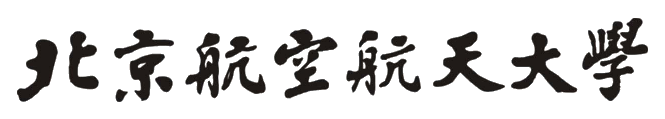
\includegraphics[width=8.8cm]{logo-buaa.eps}
\end{center}

\vspace{0.15cm}

\begin{center}

\includegraphics[width=12.8cm]{postdoc.png}
% 
\includegraphics[width=12.8cm]{postdoc1.eps}
\end{center}

\vspace{0.15cm}

\begin{center}
{\erhao\song{\bf 联邦学习中模型个性化算法研究}}
\end{center}

\vspace{0.05cm}

\begin{spacing}{2}
\begin{center}{\erhao\bf
Study of Model Personalization Methods in Federated Learning}
\end{center}
\end{spacing}

\vspace{0.05cm}

\begin{center}
{\xiaoerhao\song\boldmath\bf 文豪}
\end{center}

\vspace{0.15cm}

\begin{tabbing} %tabbing 列表

\hspace*{3cm} \= \hspace{2.6cm} \= \kill
% \= in tabbing environment, sets a tab stop
% \kill in a\tabbing environment, deletes previous line so tabs can be set without outputting text.
% \> in tabbing environment is a forward tab.
% 这次的居中 用的 \centering ,注意三次的区别。
\>{\song\sihao\textbf {研\hspace{0.3cm}究\hspace{0.3cm}方\hspace{0.3cm}向\hspace{0.3cm} :}} \>
{\centering\song\sihao\textbf{~~~~~~~~~~联邦学习~~~~~~~~~~~~~}}\\
% 总长3.4cm
\\
\>{\song\sihao\textbf {合\hspace{0.3cm}作\hspace{0.3cm}导\hspace{0.3cm}师\hspace{0.3cm} :}}\>
{\centering\song\sihao\textbf{~~~~~~~~~~韩德仁~~~~教授~~~~~~~~~~~}} \\
\\
\>{\song\sihao\textbf {工作完成日期 \ \ :}}\> {\centering\song\sihao\textbf{~~~~~~~~~~2021年3月 --- 2023年6月~~~~~~~~~~}}\\
\\
\>{\song\sihao\textbf {报告提交日期 \ \ :}}\> {\centering\song\sihao\textbf{~~~~~~~~~~2023 年6月~~~~~~~~~~}} \\

\end{tabbing}

\vspace{0.1cm}
\begin{center}
{\song\boldmath \sihao ~2023~年~6~ 月}
\end{center}


\pagenumbering{Roman}

% \newcommand{\upcite}[1]{\textsuperscript{\textsuperscript{\cite{#1}}}}

\baselineskip 18.8pt

\chapter*{摘~~~要}
\headheight=15.24pt%5mm
\markboth{摘~~~要}{摘~~~要}
\addcontentsline{toc}{chapter}{{{\hei 摘~要}}\numberline ~}
\addcontentsline{toe}{chapter}{{{Abstract in Chinese}}\numberline ~}
\pagenumbering{Roman}\setcounter{page}{1}%非常重要的命令

待写


\par
\bigskip

{\song \textbf{关键词}: 待写}

\newpage
~~~\vspace{1em}
\thispagestyle{empty}

\chapter*{{Abstract}}%\vskip1cm
 \headheight=15.24pt%5mm
\markboth{Abstract} {Abstract}
 \headheight=15.24pt%5mm
\addcontentsline{toc}{chapter}{{{\bf Abstract}}\numberline ~~~}
\addcontentsline{toe}{chapter}{{{\bf Abstract in English}}\numberline ~}
\pagenumbering{Roman}\setcounter{page}{2}

to write


\par
\bigskip

{\bf Key words:} Federated Learning, Model Personalization, Operator Splitting

%\nopagebreak[4]
\newpage
~~~\vspace{1em}
\thispagestyle{empty}



%%\mbox{}\newpage
\chapter*{\texorpdfstring{符~号~说~明}{符号说明}}
\headheight=15.24pt%5mm
\addcontentsline{toc}{chapter}{\numberline {{\heiti 符~号~说~明}}~~~}
\addcontentsline{toe}{chapter}{{{\bf Notations}}\numberline~}
\markboth{符~号~说~明}{北京航空航天大学文豪博士后研究工作报告}
%%%%%%%%%%%%%%%%%%%%%%%%%%%%%%%%%%%%%%%%%%%%%%%%%%%%%%%%%5
这里给出本文常用的一些符号, 未包含其中的符号将在文中用到时具体说明.
\begin{equation*}
\begin{array}{lll}
~\N & \qquad\qquad\qquad\qquad\qquad & \text{自然数集(包括$0$)}\\
~\R & & \text{实数集}\\
~\R^{d} & & \text{实$d$维列向量空间} \\
~\# S & & \text{有限集合$S$的元素个数} \\
% ~\R^{m\times n} & & \text{实$m \times n$矩阵的集合} \\
~\Pi_{\Omega} & & \text{向凸集$\Omega \in \R^d$投影映射} \\
~[K] & & \text{集合$\{ 1, 2, \ldots, K \},$ $K \in \N_{> 0}$} \\
~\theta & & \text{模型的参数,$\in \R^d$} \\
~\col(\theta_1, \cdots, \theta_K) & & \text{列向量$\theta_1, \ldots, \theta_K$按顺序竖排在一起形成的列向量} \\
~\operatorname{dom}(f) & & \text{函数$f$的定义域,即$\{\theta \in \R^d ~|~ f(\theta) < +\infty\}$} \\
~\nabla f(\cdot) & & \text{函数$f$的梯度} \\
~\partial f(\cdot) & & \text{函数$f$的次梯度} \\
~\mathcal{D}(x, y) & & \text{数据的分布(Distribution),} \\
& & \text{$x$是特征(Feature),$y$是标签(Label)} \\
~I_n~\text{或}~I & & \text{($n$阶)单位矩阵} \\
~O_n~\text{或}~O & & \text{($n$阶)零矩阵} \\
~A^\mathrm{T} & & \text{矩阵$A$的转置矩阵} \\
~A^{-1} & & \text{矩阵$A$的逆矩阵} \\
% \sigma(A) & & \text{矩阵$A$的谱集} \\
% \rho(A) & & \text{矩阵$A$的谱半径} \\
% \lambda_{\min}(A) & & \text{矩阵$A$的最小特征值} \\
% \lambda_{\min}^+(A) & & \text{矩阵$A$的最小正特征值} \\
% \lambda_{\max}(A) & & \text{矩阵$A$的最大特征值} \\
% \mathrm{rank}(A) & & \text{矩阵$A$的秩} \\
% \mathrm{null}(A) & & \text{矩阵$A$的零空间} \\
% \mathrm{range}(A) & & \text{矩阵$A$的值域} \\
% \mathrm{index}(A) & & \text{矩阵$A$的指标} \\
~\lVert \cdot \rVert_p & & \text{向量或矩阵的$p$-范数,$0 \leqslant p \leqslant +\infty,$} \\
& & \text{当$p$不写时,表示向量或矩阵的$2$-范数} \\
~\lVert \cdot \rVert_F & & \text{矩阵的Frobenius范数} \\
~\expectation[\cdot] & & \text{数学期望} \\
~\mathcal{N}(\mu, \sigma^2) & & \text{均值为$\mu\in\R,$ 方差为$\sigma^2\in\R$的一维正态分布} \\
~\mathcal{N}(v, \Sigma) & & \text{均值为$v\in\R^d,$ 协方差矩阵为$\Sigma\in\R^{d\times d}$的$d$维正态分布} \\
\end{array}
\end{equation*}
\nopagebreak[4]


\tableofcontents
\tableofengcontents
\mainmatter

%\mbox{}\newpage
\chapter{\hspace{-1mm}\bf 绪论及预备知识}
\label{chap1}
\addcontentsline{toe}{chapter}{{{\bf Chapter \currentchapter \ 
Introduction and Preliminaries }}\numberline\,}
\markboth{第 \currentchapter 章\ \ 
绪论及预备知识}{北京航空航天大学博士后研究工作报告}

%%%%%%%%%%%%%%%%%%%%%%%%%%%%%%%%%%%%%%%%%%%%%%%%%%%%%%%%%%%


\section{绪论}
\addcontentsline{toe}{section}{{\thecurrentchapter .1\ \ Introduction}\numberline\,}
\label{sec:chap1-introduction}

% finished
% indexed

随着人工智能 (Artificial Intelligence, AI)、大数据 (Big Data) 等技术的飞速发展,特别是物联网 (Internet of Things, IoT) 的快速普及,可用于机器学习研究的数据呈爆发式增长,其来源与分布的形式,以及来自实际应用的需求也越来越多样化。这种变化趋势给机器学习的研究与应用带来了前所未有的挑战,也提供了崭新的发展机遇。

传统上来说,机器学习的范式是将待研究的数据集中到一起,例如一个数据中心,进行统计分析、建模方法、优化算法等方面的研究。然而随着上文提到的研究数据来源与分布的形式的多样化,以及法律法规等其他因素的制约,将数据集中到一起面临越来越大的困难。举例来说,执行某一类任务的物联网设备往往数量庞大,数量级以百万乃至千万计,其产生的数据总量巨大。但是物联网设备的通信带宽往往不高,相互之间的通信,以及与数据中心之间的通信往往会有较高的延迟。在这种场景下,将感兴趣的数据集中到一起进行研究,是极其困难,成本非常高的。与此同时,随着人们的隐私保护意识越来越强,相关的法律法规,例如欧盟2018年正式生效的《General Data Protection Regulation》,越来越严格,收集用户的数据也越来越困难\citep{Albrecht_2016}。例如,用户的键盘输入数据可以用于训练输入自动补全的模型,提高用户输入效率\citep{fl_keyboard}。一般来说,通信带宽不是这类数据共享的瓶颈,但是基于隐私法律法规的限制,收集此类数据限制极大。还有一些类型的数据是具有高度机密性的数据,例如医疗、金融数据。相关的医疗机构之间或者金融机构之间往往不会进行数据共享。

在很多场景下,数据孤岛的效应比较突出:各个数据持有方持有的数据量严重不平衡,分布差异性大。如果各个数据持有方仅仅依赖各自拥有的本地数据进行模型训练,得到的机器学习模型往往是严重过拟合的,实际使用效果往往不佳。

因此,如何在尽可能地保证质量以及不进行敏感数据传输的前提下,高效率地进行分布式的机器学习模型的训练,同时使得每一个参与方都获得模型效果提升等形式的收益,最大限度的利用大数据带来的便利与优势,这一问题的重要性越来越突出。因为场景的多样性,或者说数据分布的多样性,以及相应需求的多样性,一个普适的、能满足所有需求的分布式机器学习模型训练的范式是不存在的,很多时候必须有侧重地针对某一部分需求设计相应的分布式学习方法,例如侧重隐私性的安全多方计算 (Secure Multi-Party Computation)\cite{Bogetoft_2009_smpc}\index{安全多方计算, Secure Multi-Party Computation}、差分隐私方法 (Differential Privacy)\citep{Dwork_2008_DP}\index{差分隐私, Differential Privacy}, 侧重模型训练效果的优化算法设计\citep{boyd2011distributed}等。这些问题还有很多亟待改进与完善,具有关阔的研究前景与巨大的应用价值。


\section{联邦学习的起源与演化}
\addcontentsline{toe}{section}{{1.2\ \ Origin and Development of Federal Learning}\numberline\,}
\label{sec:chap1-fl-origin}
% finished

联邦学习 Federated Learning 这个名词首次由Google的研究人员McMahan等人于2016年在文章 \emph{Communication-Efficient Learning of Deep Networks from Decentralized Data}\cite{mcmahan2017fed_avg} 中提出:
\begin{quote}
    ``We term our approach Federated Learning, since the learning task is solved by a loose federation of participating devices (which we refer to as clients) which are coordinated by a central server.''
\end{quote}
文章\parencite{mcmahan2017fed_avg}最初目的,是希望能利用用户手机端的数据改进安卓手机上输入法的预测,在防止数据泄露的前提下,基于分布在多个设备上的数据集构建机器学习模型。具有里程碑意义的综述文章 \emph{Advances and Open Problems in Federated Learning}\cite{kairouz2019advances_fl} 给联邦学习下过如下的定义
\begin{quote}
    ``Federated learning is a machine learning setting where multiple entities (clients) collaborate in solving a machine learning problem, under the coordination of a central server or service provider. Each client's raw data is stored locally and not exchanged or transferred; instead, focused updates intended for immediate aggregation are used to achieve the learning objective.''
\end{quote}
也就是说,联邦学习是一种新的机器学习范式,适用于有中心节点居中协调,多个子节点进行协作参与,进行联合建模的场景。在这种场景下,联邦学习的方法能够在每个参与方不暴露己方拥有的数据的情况下,完成联合建模的任务。一般来说,在联邦学习的框架下,数据拥有方在不用给出己方数据的情况下,也可进行模型训练得到公共的模型$M_{fed}$,使得模型$M_{fed}$,与将数据集中到一起进行训练能得到的模型$M$,二者的预测值的偏差的期望能足够小。
\begin{equation}
\label{eq:general-fl}
\expectation_{z\sim\mathcal{D}} \lVert M_{fed}(z) - M(z) \rVert \leqslant \delta.
\end{equation}
其中$\mathcal{D}$是总体训练数据的分布,$\delta$是某个我们能够接受的偏差的上界。尽管分布式优化、加密计算等问题在联邦学习这一概念被提出之前就有学者进行了研究\cite{boyd2011distributed, dist_pca_2014_nips, Gentry_2009_FHE, Nikolaenko_2013}, 但是直到联邦学习被正式提出\cite{mcmahan2017fed_avg},以上关于联邦学习独有的一些特性以及需求才真正被学界以及工业界所重视,相关的研究才开始蓬勃发展。需要注意的是,尽管文献\parencite{kairouz2019advances_fl}给出的联邦学习的定义强调了有中心节点这一特征,同时大部分关于联邦学习的文献也是基于这一假设开展研究的,但仍有一部分关于联邦学习的文献是基于无中心的完全分布式的节点网络进行研究的\cite{elgabli2020gadmm, issaid2020cq-ggadmm}.

我国杨强教授领导的香港科技大学以及微众银行(WeBank)的AI研究团队,从经济金融行业实践出发,将文献\parencite{mcmahan2017fed_avg}考虑的联邦学习经典的应用场景,即超大规模的移动、边缘设备协同参与模型训练的场景,扩展到了多个数据不互通的数据中心的场景\cite{Yang_2019_VFL}。前者被抽象为了\textbf{跨设备}(cross-device)的场景,后者被抽象为了\textbf{跨(数据)仓库}(cross-silo)的场景\cite{kairouz2019advances_fl}。跨设备的场景具有子节点数量多,每个子节点持有数据量少,算力低,通信带宽低且不稳定,对通信开销非常敏感等特点;跨仓库的场景具有子节点数量少(数量级通常在$10^2$以内),每个子节点持有数据量大,算力高,对数据的安全性、保密性要求高等特点,子节点与中心节点的通信开销与子节点本身的算力都可能成为瓶颈。这两种经过高度抽象的场景基本涵盖了联邦学习面临的所有的场景。文献\parencite{kairouz2019advances_fl}的Table 1对于这两种场景的联邦学习的特点进行了全面的总结与对比。

文献\parencite{Yang_2019_VFL}的另一个突出的贡献是从数据分布的角度,具体来说,是样本特征空间(Sample Feature Space)以及样本编号空间(Sample ID Space)的角度,将联邦学习分为三类:横向联邦学习(Horizontal Federated Learning, HFL)、纵向联邦学习(Vertical Federated Learning, VFL)和联邦迁移学习(Federated Transfer Learning, FTL)。

横向联邦学习是最常见的一类联邦学习,即每个参与方数据的特征空间基本是一致的,但各自拥有的样本编号基本是不重叠的。一般情况下,我们谈论的联邦学习,以及跨设备的联邦学习,都是横向联邦学习。纵向联邦学习则正好与横向联邦学习相反,纵向联邦学习的每个参与方有重叠度较高的样本编号空间,但是参与方之间拥有的每个样本的特征的重叠度很低。这在金融风控等领域是非常常见的。联邦迁移学习则是迁移学习(Transfer Learning)这一概念在联邦学习这一范畴内的具体应用,首先于文献\parencite{liu_2020_transfer_fl}中被系统地研究。联邦迁移学习的核心思想是,源领域(Source Domain)和目标领域(Target Domain)之间的相似性,将机器学习模型从源领域学习到的知识迁移应用到目标领域。源领域往往是知识丰富的领域(具有丰富的标签),而目标领域则是知识欠丰富,需要接受知识迁移的领域。联邦迁移学习天然适合于智慧医疗领域,例如不同医疗机构的医学影像数据一般都是不同的,但基础都是影像特征的提取与利用。

一般来说,假设一个联邦学习系统有$K$个参与方,每个参与方拥有的数据分布记作$\mathcal{D}_k.$ $\mathcal{D}_k$有分解
\begin{equation*}
\mathcal{D}_k \subseteq \mathcal{X}_k \times \mathcal{Y}_k \times \mathcal{I}_k,
\end{equation*}
其中$\mathcal{X}_k$为数据样本的特征空间(Sample Feature Space),$\mathcal{Y}_k$为数据样本的标签空间(Sample Label Space),$\mathcal{I}_k$为数据样本编号空间(Sample Feature Space)。那么有\cite{Yang_2019_VFL,vfl}
\begin{itemize}
\item 横向联邦学习:
\begin{equation*}
\mathcal{X}_i \eqabove{d} \mathcal{X}_j, ~ \mathcal{Y}_i \eqabove{d} \mathcal{Y}_j, ~ \mathcal{I}_i \neqabove{d} \mathcal{I}_j, ~ \forall i \neq j;
\end{equation*}
以上的符号$\eqabove{d}$表示相应的概率空间是同分布的。横向联邦学习一般可以简化建模为如下的最优化问题\cite{kairouz2019advances_fl}
\begin{equation}
\label{eq:general-hfl}
\begin{array}{cl}
\text{minimize} & f(\theta) = \expectation\limits_{k \sim {\mathcal{P}}} [f_k(\theta)] = \sum\limits_{k=1}^K w_k f_k(\theta), \\
\text{where} & f_k(\theta) = \expectation\limits_{(x, y) \sim \mathcal{D}_k} [\ell_k(\theta; x, y)],
\end{array}
\end{equation}
其中符号$\expectation$表示关于分布的期望,$\theta$是模型参数,也就是我们的学习目标;$\mathcal{P}$是参与训练的节点的分布,这里我们假设了总共有$K$个节点;$w_k$是节点$k$的权重,一般与节点持有的数据量正相关;$\ell_k$是节点$k$上模型训练的损失函数(Loss Function);$x, y$分别表示数据的特征与数据的标签。$f_k$以及$f$则被称作局部目标函数(Objective Function)以及全局目标函数。这里,我们忽略了数据样本编号空间,将数据分布简写为了$(x, y) \sim \mathcal{D}_k \subseteq \mathcal{X}_k \times \mathcal{Y}_k.$
\item 纵向联邦学习:
\begin{equation*}
\mathcal{X}_i \neqabove{d} \mathcal{X}_j, ~ \mathcal{Y}_i \neqabove{d} \mathcal{Y}_j, ~ \mathcal{I}_i \eqabove{d} \mathcal{I}_j, ~ \forall i \neq j;
\end{equation*}
纵向联邦学习对应的最优化模型可以写为\cite{vfl}
\begin{equation}
\label{eq:general-vfl}
\begin{array}{cl}
\text{minimize} & f(\theta) = \sum\limits_{i=1}^N \mathcal{L} \left( \mathcal{F}_K \left( \psi_K; f_{1}(\theta_{1}; x_{i}^{(1)}), \ldots, f_{K}(\theta_{K}; x_{i}^{(K)}), y_{i} \right) \right), \\
\text{where} & \theta = (\theta_{1}, \ldots, \theta_{K}), ~ x_{i} = (x_{i}^{(1)}, \ldots, x_{i}^{(K)}),
\end{array}
\end{equation}
其中$N$是总样本数,也就是说我们有$N$条数据;$x_{i}^{(k)}$为参与联邦学习的节点$k$掌握的样本$i$的部分特征,所有节点掌握的样本$i$的特征按一定规则排列构成了样本$i$的总体特征$x_{i} = (x_{i}^{(1)}, \ldots, x_{i}^{(K)}).$ 样本$i$的标签一般都假设在某一个(例如节点$K$)参与纵向联邦学习训练的节点上,这个节点被称作积极节点(Active Party),其余节点被称作被动节点(Passive Parties). 除了标签$y,$ 积极节点$K$上还拥有的直接与训练任务相关的所谓的全局模块(Global Module)$\mathcal{F}_K,$ 其参数为$\psi_K.$ 全局模块可能是简单的求平均的模块,也可以是一个神经网络的最顶层的用于最终进行回归或者分类任务的全连接层。$\mathcal{L}$是训练任务的损失函数。
\item 联邦迁移学习:
\begin{equation*}
\mathcal{X}_i \neqabove{d} \mathcal{X}_j, ~ \mathcal{Y}_i \neqabove{d} \mathcal{Y}_j, ~ \mathcal{I}_i \neqabove{d} \mathcal{I}_j, ~ \forall i \neq j;
\end{equation*}
一个有$A, B$两方参与的联邦迁移学习可以简化为如下的模型\cite{liu_2020_transfer_fl}
\begin{equation}
\label{eq:general-ftl}
\text{minimize} \quad \sum_{i=1}^{N_{AB}} \left( \ell_1(y_i^A, \varphi(u_i^B)) + \lambda \ell_2(u_i^A, u_i^B)  \right),
\end{equation}
其中$A$是源领域,$B$是目标领域;$N_{AB}$是$A, B$两方共有的样本数量;$u_i^A, u_i^B \in \mathcal{U},$ $\mathcal{U}$是$A, B$两方共有的隐式特征表示空间(Hidden Representation Space),$A, B$两方的特征通过如下的映射(例如通过两个神经网络)映到同一个空间$\mathcal{U}$
\begin{gather*}
\mathcal{X}^A \to \mathcal{U}: ~ x_i^A \mapsto u_i^A, \\ \mathcal{X}^B \to \mathcal{U}: ~ x_i^B \mapsto u_i^B.
\end{gather*}
$\ell_1$是训练任务的损失函数,$\ell_2$是所谓的对齐损失函数(Alignment Loss Function),可以取
\begin{equation*}
- \langle u_i^A, u_i^B \rangle, ~~ \text{或者} ~ \lVert u_i^A, u_i^B \rVert^2.
\end{equation*}
$\varphi$是一个所谓的翻译函数(Translator Function),用于对$u_i^B$进行打标签的,一般也可以利用隐式表示特征的相关性取作
\begin{equation}
\label{eq:ftl-translator-func}
\varphi(u_i^B) = \frac{1}{N_A} \sum\limits_{i=1}^{N_A} y_i^A \langle u_i^A, u_i^B \rangle,
\end{equation}
其中$N_{A}$是源领域$A$拥有的样本数量。
\end{itemize}
我们可以用图\ref{fig:three-types-fl}来概括地表示这三类联邦学习在以上几种概率空间上的特点。

\begin{figure}[H]
\centering
\begin{boxedminipage}{0.95\textwidth}
\centering
\begin{minipage}{0.29\textwidth}
\begin{tikzpicture}
\draw (0, 0) rectangle (3.8, 4.5);
\node at (1.95, 5.5) {横向联邦学习};
\draw[fill=pink] (0, 0) rectangle (3.5, 1.1) node[pos=.5] {client $i$};
\draw[fill=green] (0.2, 3.3) rectangle (3.8, 4.5) node[pos=.5] {client $j$};
\draw[fill=yellow] (0.3, 0.9) rectangle (3.7, 3.6) node[pos=.4] {client $k$};
\node at (1.95, -0.4) {样本特征空间};
\end{tikzpicture}
\end{minipage}
\begin{minipage}{0.29\textwidth}
\begin{tikzpicture}
\draw (0,0) rectangle (3.8, 4.5);
\node at (1.95, 5.5) {纵向联邦学习};
\draw[fill=pink] (0, 0) rectangle (1.4, 4.2) node[pos=.5, rotate=-90] {client $i$};
\draw[fill=green] (1.95, 0) rectangle (3.8, 4.5) node[pos=.5, rotate=-90] {client $j$};
\draw[fill=yellow] (1.3, 0.2) rectangle (2.1, 4.4) node[pos=.4, rotate=-90] {client $k$};
\node at (1.95, -0.4) {样本特征空间};
\end{tikzpicture}
\end{minipage}
\begin{minipage}{0.29\textwidth}
\begin{tikzpicture}
\draw (0,0) rectangle (3.8, 4.5);
\node at (1.95, 5.5) {联邦迁移学习};
\draw[fill=yellow] (0.9, 1.2) rectangle (2.2, 4.1) node[pos=.5] {client $k$};
\draw[fill=pink] (0, 0) rectangle (1.3, 1.6) node[pos=.5] {client $i$};
\draw[fill=green] (1.9, 3.6) rectangle (3.8, 4.5) node[pos=.5] {client $j$};
\node at (1.95, -0.4) {样本特征空间};
\end{tikzpicture}
\end{minipage}
\begin{minipage}{0.05\textwidth}
\begin{tikzpicture}
% \coordinate (sample_node) at (0,0);
% \node[text width=1, left=0.5cm of sample_node.west] at () {样本维度};
\node[rotate=-90] () {样本编号空间};
\end{tikzpicture}
\end{minipage}
\end{boxedminipage}
\caption{三类联邦学习的样本特征空间与样本编号空间分布的示意图}
\label{fig:three-types-fl}
\end{figure}



\section{联邦学习的应用与发展前景}
\addcontentsline{toe}{section}{{1.3\ \ Applications and Future Perspective of Federal Learning}\numberline\,}
\label{sec:chap1-fl-applications}
% finished

尽管联邦学习这一概念被提出\cite{mcmahan2017fed_avg}的时间不长,但是联邦学习已经有了不少实际的应用。我们这里仅列举一些比较重要的例子。
\begin{itemize}
    \item 首先是金融领域,联邦学习在财会\cite{Schreyer_2022_fl_audits},信贷风控\cite{Imteaj_2022_fl},反欺诈\cite{Lv_2021_fl},防范金融犯罪\cite{Toyotaro_2019_fl}等各个方面都有了实际的应用。这其中最引人注目的当属我国微众银行在这一领域的一系列前沿以及开创性的研究\cite{Yang_2019_VFL, liu_2020_transfer_fl, vfl},并以真正落地形成工业级产品的联邦学习应用框架FATE\cite{liu_2021_fate_fl}.
    \item 联邦学习在智慧医疗领域也有颇多成功应用的案例\cite{rauniyar2022_fl_medical, Antunes_2022_fl_healthcare}。从电子健康档案(Electronic Health Records, EHR)处理\cite{Brisimi_2018_fl_ehr},医学影像处理\cite{Li_2020_fl_mri},到新冠(COVID-19)等流行病的研究\cite{Dayan_2021_fl_covid},都有联邦学习的应用案例。医学因为其数据隐私性的严格要求,同时又有市场的巨大需求驱动,是联邦学习非常适宜的应用领域,同时也可能是相关研究最活跃、应用落地最多的领域之一。
    \item 移动设备、物联网领域:这是联邦学习发轫\cite{mcmahan2017fed_avg}的领域,也是大规模跨设备(Cross-Device)场景最常见的领域,应用也从最一开始的安卓设备键盘辅助输入扩展到了移动设备的语音处理\cite{Leroy_2019_fl_ks},人体活动识别(Human Activity Recognition)\cite{Sozinov_2018_fl_human},乃至人口流动预测(Human Mobility Prediction)\cite{feng_2020_fl_pmf}等问题。因为隐私性以及模型个性化(Model Personalization)等要求,很多时候联邦学习甚至是解决问题的唯一选择。
\end{itemize}

除了以上列举的一些领域外,联邦学习的应用还逐渐扩大到了智慧城市(Smart City)\cite{Zheng_2021_fl_smart_city}纳米材料\cite{Huang_2022_fl_physics}等全新的领域。可以说,联邦学习的应用场景相较于它被提出时已经得到了极大的丰富,用于仿真试验的数据集也有了很多积累。同时,也涌现出了像FedML\cite{he_2020_fedml},TensorFlow Federated\cite{tensorflow},FedSim\cite{wu_2021_fedsim},PySyft\cite{ryffel_2018_pysyft},以及之前提到的FATE\cite{liu_2021_fate_fl}等多个有不同侧重点的联邦学习软件包,为联邦学习的研究与应用落地,都提供了极大的便利。然而目前联邦学习在理论以及实际应用上,还有不少问题没有完善的解决,仍然面临着诸多的挑战\cite{kairouz2019advances_fl, Li_2020_fl_challenges}。综述性的文章\parencite{Li_2020_fl_challenges}将其总结为了4个核心的问题:
\begin{itemize}
\item 通信(Communication)开销。联邦学习往往有数量庞大的参与方,这些数量庞大的参与方可能在地理上分布极广且不均衡,这在跨设备(Cross-Device)的场景尤为常见。联邦学习各个参与方为了达到协同训练模型的目的,需要传输一些信息。这种情况下,节点之间的通信带宽是较低的,有时候节点之间用于通信的时长会远高于节点本地执行模型训练的计算时长。这就带来了极高的通信成本,使得通信成为了联邦学习的关键性瓶颈之一。联邦学习研究人员为处理这个问题提出了多项技术,如压缩传输\cite{seide2014_1bitsgd},异步更新\cite{tran2021feddr},``跳步''\cite{proxskip, zhang2020fedpd},乃至将联邦学习节点网络进行分层组成超图\cite{t2020pfedme}等。
\item 统计异质性(Systems Heterogeneity)。联邦学习的各个参与方在计算资源(CPU和内存)、网络条件(3G、4G、5G和Wi-Fi)等硬件条件是差别极大的,因此联邦学习参与方的设备在存储、计算和通信等几个方面的能力会大不相同。此外,设备的性能差异和一些系统无关的约束,例如私人手机作为参与方在工作时间无暇参与联邦学习;由于网络连接的不稳定性或设备能量限制等,有参与方设备在联邦学习训练的中途退出也是会发生的。这些系统上的特性使联邦学习的算法与系统设计需要在应对掉队者(Straggler),提高容错能力(Fault Tolerance)等方面有一定的考虑。
\item 统计异质性(Statistical Heterogeneity)。通常参与方的设备产生和收集数据的方式是有高度非一致性的。这种数据生成方式因为不满足分布式优化中经常使用的独立同分布(Independent and Identically Distributed, I.I.D.)假设,从而可能在问题建模、算法收敛性(无论是理论分析上还是实际应用上)等方面带来困难。文献\cite{kairouz2019advances_fl}对联邦学习参与方之间的数据的统计异构性做了详细的分类。我们沿用上一小节的记号,用
\begin{equation}
\label{eq:dist_decomp}
\mathcal{D}_k(x, y) = \mathcal{D}_k(y | x) \mathcal{D}_k(x) = \mathcal{D}_k(x | y) \mathcal{D}_k(y)
\end{equation}
表示联邦学习参与方$k$上的训练数据的概率分布,其中$\mathcal{D}_k(x),$ $\mathcal{D}_k(y)$分别表示样本数据特征的边缘分布以及标签的边缘分布;$\mathcal{D}_k(y | x),$ $\mathcal{D}_k(x | y)$表示条件分布。

具体来说,根据$\mathcal{D}_k(x),$ $\mathcal{D}_k(y),$ $\mathcal{D}_k(x | y),$ $\mathcal{D}_k(y | x)$的由参与方$k$的不同而带来的差别,这些统计异质性体现为
\begin{itemize}
    \item 特征分布偏斜(Feature Distribution Skew),又称协变量偏移(Covariate Shift)。这种统计的异质性是由于特征的(边缘)分布$\mathcal{D}_k(x)$在不同的参与方$K$之间不是同分布的。例如手写字体识别,不同的人写出的同一个字的字形会有区别;又例如语音识别,不同的人说同一段话也可能会有口音的差别。
    \item 标签分布偏斜(Label Distribution Skew),又称先验概率偏移(Prior Probability Shift)。这种统计的异质性是由于标签的(边缘)分布$\mathcal{D}_k(y)$不是同分布的,很多时候与样本的地域分布有较强的的关联。例如橡胶树、棕榈树等基本不会生长在高维度地区,而针叶乔木在热带地区也是极为罕见的。如果某个联邦学习系统用于植物的图像自动识别,参与方在热带、寒带地区都有分布,则很可能会发生如上的先验概率偏移现象。
    \item 概念偏移(Concept Shift),即条件分布$\mathcal{D}_k(x | y)$与$\mathcal{D}_k(y | x)$的在不同参与方$k$之间的差异性导致的。通俗来说,就是同一概念(即标签$y$),在不同参与方$k$上对应的事物(即特征$x$)可能差异极大,例如某些地区的``桥''只有形态稍有差异的简易木桥,一些地区古朴的拱式桥占多数,而又有一些区域有大量的宏伟的斜拉桥;或是同一事物(即特征$x$)在不同的参与方对应差别巨大的概念(即标签$y$),例如同样是吸食大麻的行为,在某些地区可能被认为只是一种中性的个人爱好,而在另一些地区被认为是非常恶劣的犯罪行为。
    \item 数量偏斜(Quantity Skew)。联邦学习参与方持有的数据量可能差别很大,甚至达到数量级的差异。这种情况下,公平性(Fairness)以及训练的效率等问题是不可忽视的。
\end{itemize}
在真实的联邦学习应用场景中,这几种统计上的异质性都可能会出现,会让情况变得及其复杂。因为这种统计异构性的存在,尽管经典的联邦学习问题旨在学习共享的全局模型,许多研究者投入到个性化联邦学习的研究中,这也是本文的研究重点之一。
\item 数据隐私的保护。数据的隐私性要求是联邦学习被提出的主要原因之一,也是需要考虑的基本问题。经典的联邦学习通过共享模型更新,而不是原始数据,用作保护每个参与方数据的基本手段。然而,在整个训练过程中传递模型更新可能会向第三方或中央服务器泄露敏感信息,特别是梯度信息的使用存在着使得第三方反推原始数据的可能\cite{zhu2019deep_leakage}。尽管可以使用差分隐私\cite{Dwork_2008_DP}等工具增强联邦学习对隐私的保护能力,但这些方法通常以降低模型性能或系统效率为代价。如何权衡隐私的保护与模型的性能,进行取舍,乃至从原理上进行改进,是联邦学习的一个相当大的挑战。
\end{itemize}

关于这几大挑战,还有为数众多的公开问题未得到解决。例如联邦学习在接近实际情况(即目标函数非凸,再叠加上统计异质性与系统异构性等复杂因素)下,优化算法的设计及其理论收敛性以及收敛率;个性化联邦学习的建模,优化算法迭代格式;传统优化算法,例如算子分裂算法、交替方向乘子法,在联邦学习的范畴以及框架内的适配改造与应用。这些都是联邦学习这一研究领域在未来的一段时间内要进行研究探索的重要问题。


\section{本文结构}
\addcontentsline{toe}{section}{{\thesection\ \ Structure of the Report}\numberline\,}
% \esection{Structure of the Report}
\label{sec:chap1-structure}

% almost finished

本文在第\ref{chap2}~章会先对联邦学习中已有的优化算法进行回顾,并会着重介绍其中的原始对偶(Primal-Dual)算法以及算子分裂(Operator Splitting)算法。
在接下来的第\ref{chap3}~章介绍联邦学习中的模型个性化的概念,介绍其产生的动机,已有的一些方法。
% 并在第\ref{chap4}~章引入算子分裂法来处理这个问题。
为了方便联邦学习算法的快速验证,笔者使用Python语言实现了一套联邦学习的仿真软件。这套软件的设计原则与模块会在本文的第\ref{chap5}~章中进行介绍。在接下来的第\ref{chap6}~章中,本文利用这套仿真软件进行数值实验,验证本文提出的联邦学习算法的有效性以及优越性。


%\mbox{}\newpage
\chapter{\hspace{-1mm}\bf 联邦学习中的优化算法}
\label{chap2}
\addcontentsline{toe}{chapter}{{{\bf Chapter 2\ \
Optimization Algorithms in Federated Learning }}\numberline\,}
\markboth{第\,2\,章\ \
联邦学习中的优化算法}{北京航空航天大学博士后研究工作报告}

%%%%%%%%%%%%%%%%%%%%%%%%%%%%%%%%%%%%%%%%%%%%%%%%%%%%%%%%%%%

\section{联邦学习中的优化算法概述}
\addcontentsline{toe}{section}{{2.1\ \ Overview of Optimization Algorithms in Federated Learning}\numberline\,}
\label{sec:chap2-overview}
% almost finished

优化算法自从联邦学习这一概念诞生起,便一直是相关研究的中心问题之一。联邦学习开创性的文献\parencite{mcmahan2017fed_avg}中,最重要也是最为人所熟知的便是优化算法\texttt{FederatedAveraging}(简记为\texttt{FedAvg})的提出。

联邦学习优化算法最重要的设计原则,是计算效率以及通信效率并重,甚至很多时候通信效率是更重要的一个方面。这也是联邦学习与传统的分布式优化(Distributed Optimization)最显著的区别之一。实际上,分布式优化在联邦学习被提出之前就是一个被研究得比较多的问题,从具体的问题,例如分布式主成分分析(Principal Component Analysis, PCA)\cite{dist_pca_2014_nips},到一般的算法理论\cite{boyd2011distributed}都有研究人员进行了研究。当时这些研究往往仅从计算效率以及效果出发,往往不考虑通信效率、通信保密性等问题。文献\parencite{mcmahan2017fed_avg}正是从实际问题出发,发现了这些需求,基于一种分布式梯度下降算法\cite{chen2016_revisit}(该算法在文献\parencite{mcmahan2017fed_avg}中被称作\texttt{FedSGD}算法),做了上文提到的改进而提出了\texttt{FedAvg}算法。

这里还需要强调的是,\texttt{FedAvg}相对于\texttt{FedSGD}的另一个关键的改进是,子节点与中心节点之间传输的信息,从梯度改为了模型参数。这在某种程度上规避了从梯度泄露联邦学习参与方私密训练数据\cite{zhu2019deep_leakage}的潜在风险。

联邦学习在数学上来说,其本质是一个极小化经验风险函数(Minimization of Empirical Risk Function, 见下文的式~\eqref{eq:fl-basic})的优化问题。沿用式~\eqref{eq:general-hfl}~中的记号,本文考虑的联邦学习中的优化问题,其最基本的格式如下
\begin{equation}
\label{eq:fl-basic-dist}
\begin{array}{cl}
\minimize\limits_{\theta \in \R^d} & f(\theta) = \expectation\limits_{k \sim {\mathcal{P}}} [f_k(\theta)], \\
\text{where} & f_k(\theta) = \expectation\limits_{(x, y) \sim \mathcal{D}_k} [\ell_k(\theta; x, y)],
\end{array}
\end{equation}
假设我们令$\mathcal{P} = \{1, 2, \ldots, K\},$ 则上述模型可以简记为
\begin{equation}
\label{eq:fl-basic}
\begin{array}{cl}
\minimize\limits_{\theta \in \R^d} & f(\theta) = \sum\limits_{k=1}^K w_k f_k(\theta).
\end{array}
\end{equation}
通常,为了形式简便,我们令$w_k = \frac{1}{K}.$ 对于$f$以及$f_k,$ 我们一般都假设它满足如下几条最基本的假设
\begin{itemize}
\item[(A1)] $f$以及$f_k$都是$L-$光滑的($L-$smooth, $L > 0$),亦即它们有Lipschitz-连续的梯度:
\begin{equation}
\label{eq:l-smooth}
\begin{array}{c}
\lVert \nabla f (\theta) - f (\theta') \rVert \leqslant L \lVert \theta - \theta' \rVert, \\
\lVert \nabla f_k (\theta) - f_k (\theta') \rVert \leqslant L \lVert \theta - \theta' \rVert,
\end{array}
~ \forall \theta, \theta' \in \R^d, k = 1, \ldots, K.
\end{equation}
\item[(A2)] $f$下有界(Lower Bounded):存在常数$c \in \R,$ 使得
\begin{equation}
\label{eq:lower-bounded}
f(\theta) \geqslant c > -\infty, ~ \forall \theta \in \R^d.
\end{equation}
\end{itemize}
很多时候,为了方便收敛性的分析,我们还会对目标函数的梯度进行一些假设
\begin{itemize}
\item[(A3)] 梯度有界性(Bounded Gradient):存在常数$G > 0,$ 使得
\begin{equation}
\label{eq:bdd_grad}
\lVert \nabla f_k (\theta) \rVert^2 \leqslant G^2, ~ \forall \theta \in \R^d, ~ k = 1, \ldots K.
\end{equation}
\end{itemize}
数据分布的特征(是否独立同分布,以及非独立同分布的程度)是联邦学习避免不了要考虑的问题,这也是联邦学习区别于传统的分布式优化的重要特征,这也是我们在\S\ref{sec:chap1-fl-applications}~中着重讨论过的问题。
\begin{itemize}
\item[(A4-1)] 数据独立同分布(I.I.D.):
\begin{equation}
\label{eq:iid-1}
\nabla f(\theta) = \expectation [f_k(\theta)] = \expectation\limits_{(x, y) \sim \mathcal{D}_k}[\nabla \ell_k(\theta; x, y)], ~ \forall \theta \in \R^d, ~ k = 1, \ldots K,
\end{equation}
或者,对任意$\varepsilon > 0,$ $\exists B \geqslant 0,$ 满足
\begin{equation}
\label{eq:iid-2}
\sum\limits_{k=1}^K \lVert \nabla f_k(\theta) \rVert^2 = \lVert f(\theta) \rVert^2, ~ \forall \theta \in \left\{ \theta \in \R^d ~ \middle| ~ \lVert f(\theta) \rVert^2 > \varepsilon \right\}.
\end{equation}
\item[(A4-2)] 数据非独立同分布(Non-I.I.D.),这个时候我们需要有一个量,用来度量这种统计上的异质性的程度。这个量可以有多种定义方式\cite{karimireddy2020scaffold, zhang2020fedpd, li2019convergence, sahu2018fedprox},本文采用文献\parencite{karimireddy2020scaffold}以及文献\parencite{zhang2020fedpd}中定义的梯度差异有界性(Bounded Gradient Dissimilarity),记作$(G; B)$-BGD. 具体来说,存在常数$G > 0,$ 以及$B \geqslant 0,$ 满足
\begin{equation}
\label{eq:bdd_grad_dissim}
\dfrac{1}{K} \sum\limits_{k=1}^K \lVert \nabla f_k(\theta) \rVert^2 \leqslant G^2 + B^2 \lVert \nabla f(\theta) \rVert^2, ~ \forall \theta \in \R^d.
\end{equation}
需要注意的是,如果令$B = 0,$ 那么梯度差异有界性条件~\eqref{eq:bdd_grad_dissim}~就退化为了梯度有界性条件~\eqref{eq:bdd_grad}。
\end{itemize}
很多时候,在证明算法收敛性的时候,我们需要对目标函数$f$进行一些凸性方面的假设,我们先引入相关的定义。
\begin{definition}
\label{def-convexity}
设$f: \mathcal{C} -> \R$是定义在$\R^n$中凸集(Convex Set)的连续函数,
\begin{enumerate}
\item 称$f$是凸函数(Convex Function),若有
\begin{equation}
\label{eq:def-convex-function-1}
f(a \theta + (1 - a) \theta') \leqslant a f(\theta) + (1 - a) f(\theta'), ~ \forall \theta, \theta' \in \mathcal{C}, ~ \alpha \in [0, 1].
\end{equation}
\item 称$f$是$\mu$-强凸函数($\mu$-Strongly Convex Function),$\mu > 0,$ 若$f - \frac{\mu}{2} \lVert \theta \rVert^2$是凸函数。
\end{enumerate}
如果$\mathcal{C}$是开集,而且$f$在$\mathcal{C}$上可微,那么以上关于函数凸性以及强凸性的定义式可分别写为
\begin{equation}
\label{eq:def-convex-function-2}
f(\theta') \geqslant f(\theta) + \langle \theta' - \theta, \nabla f (\theta) \rangle
\end{equation}
以及
\begin{equation}
\label{eq:def-strongly-convex-function}
f(\theta') \geqslant f(\theta) + \langle \theta' - \theta, \nabla f (\theta) \rangle + \frac{\mu}{2} \lVert \theta' - \theta \rVert^2
\end{equation}
\end{definition}

由于联邦学习天然的分层以及可解耦的结构(见\S\ref{sec:chap1-fl-origin}),更方便以及自然的做法,是将问题~\eqref{eq:fl-basic}~写成约束优化问题的格式:
\begin{equation}
\label{eq:fl-basic-constraint}
\begin{array}{cl}
\minimize & \sum\limits_{k=1}^K w_k f_k(\theta_k), \\
\text{subject to} & \theta_k = \theta, ~ k = 1, \ldots, K.
\end{array}
\end{equation}
我们很容易看出~\eqref{eq:fl-basic-constraint}~与~\eqref{eq:fl-basic}~这两种格式的等价性。格式\eqref{eq:fl-basic-constraint}~在分布式优化中被称作共识问题(Consensus Problem)。我们会在本文随后的章节发现,约束优化的格式~\eqref{eq:fl-basic-constraint}~及其变体,更有利于我们对算法进行理论分析,进而对算法的改进做出指导。

\subsection{联邦平均算法}
\label{subsec:chap2-overview-fedavg}

联邦平均算法(Federated Averaging Algorithm)\cite{mcmahan2017fed_avg}是首个被提出的联邦学习算法,后续一系列的工作都是以此为基础进行的改进。我们先给出该算法的伪代码\ref{algo:fedavg}。

\begin{algorithm}[ht]
% \SetAlgoNoLine
% \DontPrintSemicolon
\SetKwInOut{Input}{Input}
\Input{learning rate $\eta$, batch size $B$}
{\bfseries Server executes:}\;
\Indp
{\bfseries Initiation:} parameters $\theta^{(0)}$\;
\For{each round $t = 0, 1, \cdots, T-1$}{
    $S^{(t)} \gets$ (random set of clients)\;
    \For{each client $k \in \mathcal{S}^{(t)}$ {\bfseries in parallel}}{
        $\theta_k^{(t)} \gets$ {\bfseries ClientUpdate}$(k, \theta^{(t)})$\;
        }
    $\theta^{(t+1)} \gets \frac{1}{\lvert \mathcal{S}^{(t)} \rvert} \sum\limits_{k\in \mathcal{S}^{(t)}} \theta_k^{(t)}$\;
}
\Indm
\vspace{0.2em}
{\bfseries ClientUpdate}$(k, \theta)$: \tcc*[h]{on client $k$}\;
\Indp $\mathcal{B} \gets$ (split $\mathcal{D}_k$ into batches of size $B$)\;
\For{local step $r = 0, 1, \cdots, R-1$}{
    \For{batch $b \in \mathcal{B}$}{
        $\theta \gets \theta - \eta \nabla \ell_k(\theta; b)$ \tcc*[h]{SGD} \;
    }
}
return $\theta$\;
\caption{联邦平均(FedAvg)\cite{mcmahan2017fed_avg}算法的伪代码}
\label{algo:fedavg}
\end{algorithm}


联邦平均算法的核心思想,是充分利用子节点的计算能力,在以学习率(learning rate, 又称步长,step size) $\eta$执行完一定轮数的随机梯度下降(Stochastic Gradient Descent, SGD)\cite{Robbins_1951_sgd}之后,由中心节点收集各子节点发送过来的模型参数,进行平均(Averaging),之后再将平均之后的模型参数广播(Broadcast)给子节点进行下一轮迭代。这样,规避了每一轮SGD都进行通信带来的巨大的通信开销,在加速模型训练的同时,数值上在某些情况下还有更好的收敛性。这实际上是一种比较朴素与简单的``跳步''的思想,这种思想也在随后的研究\cite{zhang2020fedpd, proxskip, proxskip-vr}也得到了进一步的发展。

联邦平均算法在数值上取得了一些不错的实验结果\cite[Section 3]{mcmahan2017fed_avg},但是其收敛性,特别是在数据非独立同分布的情况下,并未得到证明。后续的文献\parencite{zhou_2018_convergence}首先在假设数据独立同分布的情况下证明了联邦平均算法的收敛性。文献\parencite{li2019convergence}进一步在非独立同分布的情况下证明了联邦平均算法的收敛性,但添加了$f$强凸(见定义\ref{def-convexity})的假设。

% TODO: 看这里是否要列举一些收敛率的定理

\subsection{最优化理论视角下的联邦平均算法}
\label{subsec:chap2-overview-fedavg-opt}

我们从最优化理论的角度对联邦平均算法进行分析。事实上,联邦平均算法处理的优化问题~\eqref{eq:fl-basic}~可以等价地改写为如下的约束优化问题(注意与格式\ref{eq:fl-basic-constraint}~的差别)
\begin{equation}
\label{eq:fedavg-constraint}
\begin{array}{cl}
\minimize & F(\Theta) := \sum\limits_{k=1}^K w_k f_k(\theta_k), \\
\text{subject to} & \Theta \in \mathcal{E},
\end{array}
\end{equation}
其中$\Theta = \begin{pmatrix} \theta_1 \\ \vdots \\ \theta_K \end{pmatrix}, \theta_1, \ldots, \theta_K \in \R^d,$ $\mathcal{E} = \left\{ \Theta ~ \middle| ~ \theta_1 = \cdots = \theta_K \right\}$是$\R^{Kd}$中一个凸集。我们知道,投影梯度下降法(Projected Gradient Descent)是求解问题~\eqref{eq:fedavg-constraint}~的一个有效的算法。投影梯度下降法的迭代格式是
\begin{equation}
\label{eq:fedavg-pgd}
\Theta^{(t+1)} = \Pi_{\mathcal{E}} \left( \Theta^{(t)} - \eta \nabla F(\Theta^{(t)}) \right),
\end{equation}
其中$\Pi_{\mathcal{E}}$是到集合$\mathcal{E}$的投影算子。容易看出,到集合$\mathcal{E} = \left\{ \Theta ~ \middle| ~ \theta_1 = \cdots = \theta_K \right\}$的投影映射就是``求平均''映射:
\begin{equation*}
\Pi_{\mathcal{E}}: \R^{Kd} \to \mathcal{E}: (\theta_1, \ldots, \theta_K) \mapsto (\frac{1}{K}\sum\limits_{k=1}^K \theta_K, \ldots, \frac{1}{K}\sum\limits_{k=1}^K \theta_K).
\end{equation*}
也就是说联邦平均算法在数学上,实质上是一种随机投影梯度法,子节点执行的是梯度步(具体来说是用的随机梯度下降),中心节点执行的是投影步。

% 关于联邦平均算法\texttt{FedAvg}的收敛结果,待写。。。

\subsection{联邦平均算法的改进}
\label{subsec:chap2-overview-fedavg-improve}

收敛速度是最优化算法的一个重要指标,自从联邦平均算法\texttt{FedAvg}算法被提出以来,一直有学者从联邦学习面临的几大核心挑战(见\S\ref{sec:chap1-fl-applications})出发,对联邦平均算法加以改进,提出一些收敛速度更快\cite{reddi2020fed_opt}、通信资源要求更少\cite{karimireddy2020scaffold}、鲁棒性更强\cite{sahu2018fedprox}的算法。

因为联邦平均算法是以随机梯度下降法为基础的,那么一个自然的想法就是将随机梯度下降法的一些加速的技巧\cite{adagrad, adam, Zaheer_2018_yogi, adamw_amsgrad}引入联邦学习整个算法体系内。由于联邦学习子节点与中心节点的计算相对独立无耦合,所以这种做法并不需要对联邦学习整个算法框架做大改动,是一种可行的方法。事实上,联邦平均算法的作者在随后发表的文章\parencite{reddi2020fed_opt}中实践了这一想法,提出了一个泛用性更强的\texttt{FedOpt}的联邦学习算法框架。\texttt{FedOpt}的伪代码见算法\ref{algo:fedopt}. 

\begin{algorithm}[ht]
% \SetAlgoNoLine
% \DontPrintSemicolon
\SetKwInOut{Input}{Input}
\Input{methods {\bfseries ServerOpt, ClientOpt}, learning rates (schedule) $\eta_g, \eta_l$}
{\bfseries Initiation:} global model parameters $\theta^{(0)}$\;
\For{each round $t = 0, 1, \cdots, T-1$}{
    $S^{(t)} \gets$ (random set of clients)\;
    \For{each client $k \in S^{(t)}$ {\bfseries in parallel}}{
        $\theta_k^{(t, 0)} \gets \theta^{(t)}$\;
        \For{local step $r = 0, 1, \cdots, R-1$}{
            Compute unbiased estimate $g_k^{(t, r)}$ of $\nabla f_k(\theta_k^{(t, r)})$\;
            $\theta_k^{(t, r+1)} \gets$ {\bfseries ClientOpt}$(\theta_k^{(t, r)}, g_k^{(t, r)}, \eta_l, t)$\;
        }
        $\Delta_{k}^{(t)} \gets \theta_k^{(t, R)} - \theta^{(t)}$
    }
    {\bfseries Server Update:}\;
    \Indp
    $\Delta^{(t)} \gets \operatorname{aggregate} \left( \left\{ \Delta_{k}^{(t)} \right\}_{k \in \mathcal{S}^{(t)}} \right)$\;
    $\theta^{(t+1)} \gets$ {\bfseries ServerOpt}$(\theta^{(t)}, \Delta^{(t)}, \eta_g, t)$\;
}
\caption{\texttt{FedOpt}\cite{reddi2020fed_opt}算法的伪代码}
\label{algo:fedopt}
\end{algorithm}


这里的$\operatorname{aggregate} \left( \left\{ \Delta_{k}^{(t)} \right\}_{k \in \mathcal{S}^{(t)}} \right)$指的是将来自子节点的惯性项$\Delta_{k}^{(t)}$聚合为全局惯性量的方法,例如可以采用简单的均值
\begin{equation*}
\Delta^{(t)} \gets \frac{1}{\lvert \mathcal{S}^{(t)} \rvert} \sum\limits_{k \in \mathcal{S}^{(t)}} \Delta_{k}^{(t)}
\end{equation*}
或者与上一步惯性量的线性组合
\begin{equation*}
\Delta^{(t)} \gets \beta_1 \Delta^{(t-1)} + \left( (1 - \beta_1) / \lvert \mathcal{S}^{(t)} \rvert \right) \sum_{k \in \mathcal{S}^{(t)}} \Delta_{k}^{(t)}
\end{equation*}

我们注意到,相比于\texttt{FedAvg}算法\ref{algo:fedavg},\texttt{FedOpt}在中心节点引入了带动量(Momentum)的项用于\textbf{ServerOpt}进行加速。我们列举一些\textbf{ServerOpt}可供选择的方法\cite{reddi2020fed_opt}:
\begin{itemize}
    \item \texttt{FedAdagrad}:
    \begin{equation*}
    \begin{aligned}
    v^{(t)} & \gets v^{(t-1)} + ( \Delta^{(t)} )^2 \\
    \theta^{(t+1)} & \gets \theta^{(t)} + \eta_g \Delta^{(t)} / (\sqrt{v^{(t)}}+\tau)
    \end{aligned}
    \end{equation*}
    \item \texttt{FedYogi}:
    \begin{equation*}
    \begin{aligned}
    v^{(t)} & \gets v^{(t-1)} - (1 - \beta_2) ( \Delta^{(t)} )^2 \operatorname{sign}(v^{(t-1)} - ( \Delta^{(t)} )^2) \\
    \theta^{(t+1)} & \gets \theta^{(t)} + \eta_g \Delta^{(t)} / (\sqrt{v^{(t)}}+\tau)
    \end{aligned}
    \end{equation*}
    \item \texttt{FedAdam}:
    \begin{equation*}
    \begin{aligned}
    v^{(t)} & \gets \beta_2 v^{(t-1)} + (1 - \beta_2) ( \Delta^{(t)} )^2 & \gets \theta^{(t)} + \eta_g \Delta^{(t)} / (\sqrt{v^{(t)}}+\tau)
    \end{aligned}
    \end{equation*}
\end{itemize}

\texttt{FedOpt}将机器学习领域内常用的一些加速的技巧应用于联邦学习的场景,是\texttt{FedAvg}较为平凡的推广,它的另一个更重要的意义在于充分表明了联邦学习子节点与中心节点的计算的解耦合的性质。

\texttt{FedAvg}以及\texttt{FedOpt}算法考虑的主要是数据在各子节点之间独立同分布的场景。对于更具有实际意义的数据非独立同分布的场景,我们需要引入一些别的工具来处理这种情况。此时,各子节点上的梯度在分布上是有差异的,一个很自然的想法就是引入一些额外的参数,与模型参数一起更新,利用这些额外的参数对子节点的梯度进行修正,减小各子节点上的梯度在分布上的差异,进而达到使算法收敛更稳定以及加速收敛的目的。这种技术就是方差缩减(Variance Reduction)技术\cite{johnson2013accelerating},由文献\parencite{karimireddy2020scaffold}以算法\texttt{SCAFFOLD} (Stochastic Controlled Averaging algorithm) 的形式首次引入联邦学习中,其伪代码可见算法\ref{algo:scaffold}。

\begin{algorithm}[ht]
% \SetAlgoNoLine
% \DontPrintSemicolon
\SetKwInOut{Input}{Input}
\Input{server learning rate $\eta_g,$ client learning rates $\eta_k,$ $\forall k \in [K]$}
{\bfseries Initiation:}\;
\Indp
    {\bfseries Server init:} global model parameters $\theta^{(0)} \in \R^d,$ control variates $c^{(0)} \in \R^d$\;
    {\bfseries Clients init:} control variates $c_k^{(0)} \in \R^d, ~ \forall k \in [K]$\;
\Indm
\For{each round $t = 0, 1, \cdots, T-1$}{
    $S^{(t)} \gets$ (random set of clients) $\subseteq [K]$\;
    broadcast $(\theta^{(t)}, c^{(t)})$ to clients $k \in S^{(t)}$\;
    \For{each client $k \in S^{(t)}$ {\bfseries in parallel}}{
        $\theta_k^{(t, 0)} \gets \theta^{(t)}$\;
        \For(\tcc*[h]{$R$ iterates of SGD with variance reduction}){local step $r = 0, 1, \cdots, R-1$}{
            compute mini-batch gradient $g_k^{(t, r)}$ of $\nabla f_k(\theta_k^{(t, r)})$\;
            $\theta_k^{(t, r+1)} \gets \theta_k^{(t, r)} - \eta_k \left( g_k^{(t, r)} - c_k^{(t)} + c^{(t)} \right)$\;
        }
        $c_k^{(t+\frac{1}{2})} \gets \begin{cases} \text{Option 1} & g_k^{(t, 0)} \\ \text{Option 2} & c_k^{(t)} - c^{(t)} + \frac{1}{R\eta_k} \left( \theta^{(t)} - \theta_k^{(t, R)} \right) \end{cases}$\;
        $( \Delta \theta_k^{(t)}, \Delta c_k^{(t)} ) \gets ( \theta_k^{(t, R)} - \theta^{(t)}, c_k^{(t+\frac{1}{2})} - c_k^{(t)} )$\;
        send $( \Delta \theta_k^{(t)}, \Delta c_k^{(t)} )$ to server\;
        $c_k^{(t+1)} \gets c_k^{(t+\frac{1}{2})}$\;
    }
    {\bfseries Server Update:}\;
    \Indp
    $( \Delta \theta^{(t)}, \Delta c^{(t)} ) \gets \frac{1}{\lvert S^{(t)} \rvert} \sum\limits_{k \in S^{(t)}} ( \Delta \theta_k^{(t)}, \Delta c_k^{(t)} )$\;
    $\theta^{(t+1)} \gets \theta^{(t)} + \eta_g \Delta \theta^{(t)}$\;
    $c^{(t+1)} \gets c^{(t)} + \frac{\lvert S^{(t)} \rvert}{K} \Delta c^{(t)}$\;
}
\caption{\texttt{SCAFFOLD} (Stochastic Controlled Averaging) 算法\cite{karimireddy2020scaffold}的伪代码}
\label{algo:scaffold}
\end{algorithm}


方差缩减这项技术可以灵活地和大部分算法相结合,目前已经成为联邦学习中统计异质性的一种常用的处理手段。需要注意的是,我们可以在\texttt{SCAFFOLD}算法\ref{algo:scaffold}~中看到,在中心服务器端与子节点端,都有额外的参数$c, c_k$需要维护,产生额外的通信开销。这对于在通信开销敏感的联邦学习场景,这会是一个潜在的问题,所以一个更好的办法是将方差缩减与``跳步''更新的技术联合使用\cite{proxskip-vr}。关于``跳步''的算法,我们会在\S\ref{sec:chap2-skip-alg}~中进行更详细的介绍。同时,\texttt{SCAFFOLD}算法\ref{algo:scaffold}~传输了梯度相关的信息,这在安全性方面\cite{zhu2019deep_leakage}也是一个隐患。


\section{联邦学习中的临近点算法}
\addcontentsline{toe}{section}{{2.2\ \ Proximal Point Algorithms in Federated Learning}\numberline\,}
\label{sec:chap2-ppa}

基于减小数据非独立同分布情形下,每一轮的子节点更新对整体模型的影响,文献\parencite{sahu2018fedprox}首先提在子节点上的局部模型中增加邻近项的联邦临近点算法\texttt{FedProx},达到了算法收敛更快、更加稳定的目的。相较于\texttt{SCAFFOLD}算法\ref{algo:scaffold},使用临近项的方案不需要进行额外(关于梯度信息)参数的维护与传递,没有通信开销以及安全性上的额外代价。

具体来说,在算法迭代的第$t+1$轮,每个子节点优化的目标函数从$f_k(\theta_k)$变为了如下的带临近项的函数
\begin{equation}
\label{eq:fedprox}
h_k(\theta_k, \theta^{(t)}) := \left\{ f_k(\theta_k) + \frac{\mu}{2} \lVert \theta_k - \theta^{(t)} \rVert^2  \right\},
\end{equation}
上式中的$\mu$被称作罚参数(Penalty Constant)。值得注意的是,上式临近项的中心为$\theta^{(t)},$ 即上一轮迭代得到的全局模型。关于临近项中心的其他选取,文献\parencite{hanzely2020federated,li_2021_ditto}进行了研究,我们随后进行详细介绍。我们将联邦临近点算法\texttt{FedProx}的伪代码总结在算法\ref{algo:fedprox}~中。

\begin{algorithm}[!htb]
% \SetAlgoNoLine
% \DontPrintSemicolon
\SetKwInOut{Input}{Input}
\Input{penalty constant $\mu,$ constant $\gamma \in [0, 1]$}
{\bfseries Initiation:} global model parameters $\theta^{(0)} \in \R^d$\;
\For{each round $t = 0, 1, \cdots, T-1$}{
    $\mathcal{S}^{(t)} \gets$ (random set of clients) $\subseteq [K]$\;
    broadcast $\theta^{(t)}$ to clients $k \in \mathcal{S}^{(t)}$\;
    \For{each client $k \in \mathcal{S}^{(t)}$ {\bfseries in parallel}}{
        find a $\gamma$-inexact solution $\theta_k^{(t)}$ to $\argmin\limits_{\theta_k} h_k(\theta_k, \theta^{(t)}) := f_k(\theta_k) + \frac{\mu}{2} \lVert \theta_k - \theta^{(t)} \rVert^2.$\;
        \tcc{Definition of $\gamma$-inexactness: $\nabla h_k(\theta_k^*, \theta^{(t)}) \leqslant \gamma h_k(\theta_k, \theta^{(t)}),$ where $\theta_k^*$ is the exact solution to $h_k.$}
        send $\theta_k^{(t)}$ to server\;
    }
    {\bfseries Server Update:}\;
    \Indp
    $\theta^{(t+1)} \gets \frac{1}{\lvert \mathcal{S}^{(t)} \rvert} \sum\limits_{k\in \mathcal{S}^{(t)}} \theta_k^{(t)}$\;
    \Indm
}
\caption{联邦临近算法\texttt{FedFrox}\cite{sahu2018fedprox}的伪代码}
\label{algo:fedprox}
\end{algorithm}


我们把$\gamma$-非精确解$\theta_k^{(t)}$记作
\begin{equation}
\label{eq:prox-op}
\theta_k^{(t)} \approx \prox_{f_k, \mu} (\theta^{(t)}) := \argmin\limits_{\theta_k} \left\{ f_k(\theta_k) + \frac{\mu}{2} \lVert \theta_k - \theta^{(t)} \rVert^2 \right\},
\end{equation}
其中的$\prox_{f_k, \mu}$为临近算子(Proximity Operator)\cite{Moreau_1965_prox}。令$s = \frac{1}{\mu},$ 因为$\prox_{f_k, \mu} = \prox_{sf_k, 1},$ 我们也把$\prox_{f_k, \mu}$记为$\prox_{sf_k}.$ 相应的函数
\begin{equation}
\label{eq:moreau_env}
\mathcal{M}_{sf_k} (\theta^{(t)}) = \mathcal{M}_{f_k, \mu} (\theta^{(t)}) := \inf\limits_{\theta_k} \left\{ f_k(\theta_k) + \frac{\mu}{2} \lVert \theta_k - \theta^{(t)} \rVert^2 \right\}
\end{equation}
被称作$f_k$的Moreau包络(Moreau Envelope)或者Moreau-Yosida正规化(Moreau-Yosida Regularization)。函数$f_k$的Moreau包络与它的临近算子有如下关系\cite{Parikh_2014_pa}
\begin{equation*}
\prox_{sf_k} (\theta_k) = \theta_k - s \nabla \mathcal{M}_{sf_k} (\theta_k),
\end{equation*}
也就是说,$\prox_{sf_k}$可以视作是以$s$为步长进行的极小化函数$\mathcal{M}_{sf_k}$的梯度下降算子。

关于联邦临近点算法\texttt{FedProx}在非凸情况下的收敛性,文献\parencite{sahu2018fedprox}有如下的结论
\begin{theorem}[\parencite{sahu2018fedprox} Theorem 4]
\label{thm:fedprox}
假设子节点的目标函数$\{f_k\}_{k=1}^K$都是非凸、$L$−光滑(定义见式~\eqref{eq:l-smooth})函数,并且存在常数$L_- > 0,$使得$\nabla^2 f_k \succcurlyeq -L_- I_d.$ 又假设$\{f_k\}_{k=1}^K$满足差异有解条件(Bounded Dissimilarity),即对$\varepsilon > 0,$ 存在常数$B_{\varepsilon} > 0,$ 使得集合$\mathcal{S}_{\varepsilon}^c := \{ \theta ~|~ \lVert \nabla f(\theta) \rVert^2 > \varepsilon\}$中的任何一点$\theta$都满足不等式
\begin{equation}
\label{eq:fedprox_bdd_dissim}
B(\theta) := \frac{\expectation_k [\lVert \nabla f_k(\theta) \rVert^2]}{\lVert \nabla f(\theta) \rVert^2} \leqslant B_{\varepsilon}.
\end{equation}
选取常数$\mu, \gamma$满足
\begin{equation*}
\rho := \left( \frac{1}{\mu} - \frac{\gamma B}{\mu} - \frac{B(1+\gamma)\sqrt{2}}{\bar{\mu}\sqrt{K}} - \frac{LB(1+\gamma)}{\bar{\mu}\mu} - \frac{LB^2(1+\gamma)^2}{2\bar{\mu}^2} - \frac{LB^2(1+\gamma)^2}{\bar{\mu}^2 K} \left( 2\sqrt{2K} + 2 \right) \right) > 0,
\end{equation*}
其中$\bar{\mu} = \mu - L_- > 0.$ 那么在联邦临近点算法\ref{algo:fedprox}~的第$t+1$步,设前一步的全局模型参数$\theta^{(t)}$为全局目标函数$f$的一阶非稳定点(即$\theta^{(t)} \in \mathcal{S}_{\varepsilon}^c,$ 那么$f$的值满足如下的下降关系
\begin{equation*}
\expectation\nolimits_{\mathcal{S}^{(t)}}[f(\theta^{(t+1)})] \leqslant f(\theta^{(t)}) - \rho \lVert \nabla f (\theta^{(t)}) \rVert^2.
\end{equation*}
\end{theorem}

\begin{rem}
对于联邦临近点算法\texttt{FedProx}收敛性定理\ref{thm:fedprox},我们有如下的观察:在$\lVert \nabla f \rVert$的零点附近,如果这个零点没有被$\mathbb{E}_k[\lVert \nabla f_k \rVert]$消除掉,即这个点也是$\mathbb{E}_k[\lVert \nabla f_k \rVert]$的零点,且零点的阶数相同或更高,那么在这个点的邻域内,$B_{\varepsilon}$会随着$\varepsilon \to 0$而急速趋向于无穷,导致在$\lVert \nabla f \rVert$的零点附近,$\rho > 0$的假设不再成立,那么定理中的不等式就变得无意义。

当子节点之间的数据分布完全一致的时候(理想情况下),$B_{\varepsilon}$恒为1,就不会有这个问题。这也是后续一系列文章\cite{pathak2020fedsplit,tran2021feddr}进行改进的出发点。
\end{rem}

联邦临近点算法\texttt{FedProx}的积极意义在于,首次将临近点算法(Proximal Point Algorithms, PPA)引入联邦学习领域中,虽然临近点算法只是用做了(内循环问题的)子节点上的子问题的求解器,而\texttt{FedProx}算法整体严格意义上来看并不是临近点算法。临近点算法不仅仅在理论分析上可以提供一个好的框架,在算法设计上也能提供一个支撑。后续在\$\ref{chap3}~中我们将要详细研究的有关个性化联邦学习的工作\cite{hanzely2020federated,acar2021feddyn,li_2021_ditto,t2020pfedme,li2021pfedmac}都依赖于引入临近项(或者类似的项)作为模型个性化的主要技术手段。关于临近点算法本身在联邦学习的进一步研究,也有将临近点算法与方差缩减技术相结合(\texttt{FedProxVR}算法)\cite{Dinh_2020_FL_PSVRG}等方面的工作。



\section{联邦学习中的原始对偶算法}
\addcontentsline{toe}{section}{{\thesection\ \ Primal-Dual Algorithms in Federated Learning}\numberline\,}
% \esection{Primal-Dual Algorithms in Federated Learning}
\label{sec:chap2-primal-dual}

% almost finished
% indexed

在传统的最优化方法中,原始-对偶算法 (Primal-Dual Algorithms)\index{原始-对偶算法, Primal-Dual Algorithms} 也是一类常用的算法。我们考虑格式为~\eqref{eq:fl-basic-constraint}~的带等式线性约束的共识优化问题 (注意与~\eqref{eq:fl-basic-constraint}~的细微差别)
\begin{equation}
\label{eq:fedpd-constraint}
\begin{array}{cl}
\minimize & F(\Theta) := \sum\limits_{k=1}^K f_k(\theta_k), \\
\text{subject to} & \theta_k = \theta, ~ k = 1, \ldots, K.
\end{array}
\end{equation}
其中$\Theta = \col(\theta_1, \cdots, \theta_K), ~ \theta, \theta_1, \ldots, \theta_K \in \R^d.$ 约束优化问题~\eqref{eq:fedpd-constraint}~的增广拉格朗日函数 (Augmented Lagrangian, AL)\index{增广拉格朗日函数, Augmented Lagrangian, AL} 为
\begin{equation}
\label{eq:al}
\mathcal{L}(\theta, \Theta, \Lambda) = F(\Theta) - \sum\limits_{k=1}^K \left\{ \langle \lambda_k, \theta_k \rangle + \frac{1}{2s} \lVert \theta_k - \theta \rVert^2 \right\} = \sum\limits_{k=1}^K \mathcal{L}_k(\theta, \theta_k, \lambda_k)
\end{equation}
其中
\begin{equation}
\label{eq:al-local}
\mathcal{L}_k(\theta, \theta_k, \lambda_k) = f_k(\theta_k) + \langle \lambda_k, \theta_k - \theta \rangle + \frac{1}{2s} \lVert \theta_k - \theta \rVert^2,
\end{equation}
$\Lambda = \col(\lambda_1, \ldots, \lambda_K)$被称作对偶变量 (Dual Variable)\index{对偶变量, Dual Variable} 或者拉格朗日乘子 (Lagrangian Multiplier)\index{拉格朗日乘子, Lagrangian Multiplier}。通过将梯度提升算法应用到对偶问题
\begin{equation}
\label{eq:al-dual}
\text{maximize} \quad G(\Lambda) := \inf\limits_{\theta, \Theta} \mathcal{L}(\theta, \Theta, \Lambda)
\end{equation}
可以得到解这种形式的问题算法的一般迭代格式
\begin{subequations}
\label{eq:al-iter}
\begin{align}
\theta_k^{(t+1)} & = \argmin_{\theta_k} \mathcal{L}_k(\theta^{(t)}, \theta_k, \lambda_k^{(t)}) \label{eq:al-iter-local} \\
\lambda_k^{(t+1)} & = \lambda_k^{(t)} + \frac{1}{s} (\theta_k^{(t+1)} - \theta^{(t)}) \label{eq:al-iter-dual} \\
\theta^{(t+1)} & = \argmin_{\theta} \sum\limits_{k=1}^K \left\{ \frac{1}{2s} \lVert \theta_k^{(t+1)} - \theta \rVert^2 - \langle \lambda_k^{(t+1)}, \theta \rangle \right\} \nonumber \\
& = \frac{1}{K} \sum\limits_{k=1}^K (\theta_k^{(t+1)} + s\lambda_k^{(t+1)}) \label{eq:al-iter-global}
\end{align}
\end{subequations}

基于这种迭代格式,文献\parencite{zhang2020fedpd}设计了联邦原始对偶算法 (Federated Primal-Dual)\texttt{FedPD}\index{联邦原始对偶算法, \texttt{FedPD}},其伪代码可见算法~\ref{algo:fedpd}。

\begin{algorithm}[!htb]
% \SetAlgoNoLine
% \DontPrintSemicolon
\SetKwInOut{Input}{Input}
\Input{step size $s = \frac{1}{\mu} > 0,$ skip probability $p \in [0, 1)$}
{\bfseries Initiation:}\;
\Indp
    {\bfseries Init server:} global parameters $\theta^{(0)} \in \R^d$\;
    {\bfseries Init clients:} local parameters$\theta_{k,0}^{(0)} \in \R^d,$ dual variables $\lambda_k^{(0)} \in \R^d,$ $\forall k \in [K]$\;
\Indm
\For{each round $t = 0, 1, \cdots$}{
    \For{each client $k = 1, \cdots, K$ {\bfseries in parallel}}{
        $\theta_k^{(t+1)} \gets \operatorname{\mathbf{Oracle}}_k(\mathcal{L}_k(\theta_{k,0}^{(t)}, \theta_k, \lambda_k^{(t)}), \theta_k^{(t)})$  \tcc*[h]{$\operatorname{\mathbf{Oracle}}_k$ can be SGD, etc.}\;
        $\lambda_k^{(t+1)} \gets \lambda_k^{(t)} + \frac{1}{s} (\theta_k^{(t+1)} - \theta_{k,0}^{(t)})$ \tcc*[h]{dual update step}\;
        $\theta_{k,0}^{(t+\frac{1}{2})} \gets \theta_k^{(t+1)} + s \lambda_k^{(t+1)}$
        }
    with probability $1 - p$ do global communication\;
    \Indp
    client $k$ send $\theta_{k,0}^{(t+\frac{1}{2})}$ to server $\forall k \in [K]$\;
    {\bfseries Server Update:} $\theta^{(t+1)} \gets \frac{1}{K} \sum\limits_{k=1}^K \theta_{k,0}^{(t+\frac{1}{2})}$ \tcc*[h]{compute global average}\;
    Server broadcast $\theta^{(t+1)}$ to clients $k \in [K]$\;
    On client $k:$ $\theta^{(t+1)}_{k,0} \gets \theta^{(t+1)}, ~ \forall k \in [K]$\;
    \Indm
    with probability $p$ skip global communication:\;
    \Indp
    {\bfseries Client Update:} $\theta^{(t+1)}_{k,0} \gets \theta_{k,0}^{(t+\frac{1}{2})}, ~ \forall k \in [K]$\;
    \tcc{On server, $\theta^{(t+1)} \gets \theta^{(t)}$}
    \Indm
}
\caption{联邦原始对偶算法\texttt{FedPD}\cite{zhang2020fedpd}的伪代码}
\label{algo:fedpd}
\end{algorithm}


联邦原始对偶算法\texttt{FedPD}有以下几点是值得注意的。

首先,在子节点执行本地模型更新,也就是求解问题~\eqref{eq:al-iter-local}~时,\texttt{FedPD}采用了比较灵活的设置,即允许子节点上的求解器
\begin{equation*}
\operatorname{\mathbf{Oracle}}_k(\mathcal{L}_k(\theta_{k, 0}^{(t)}, \theta_k, \lambda_k^{(t)}), \theta_k^{(t)})
\end{equation*}
可以是任何一个求解算法,例如随机梯度下降,亦或是与在SCAFFOLD算法~\ref{algo:scaffold}~中应用过的方差缩减技术进行结合。这种灵活性,是联邦学习的显著特点,这一点我们已经在\S~\ref{sec:chap2-overview}~中介绍\texttt{FedOpt}算法的时候已经强调过了。文献\parencite{zhang2020fedpd}进一步特别提到的是,在方差缩减技术的时候,可以进一步结合线性化的方法进行加速,即把需要优化的 (局部) 拉格朗日函数进行线性化,或者更准确的说,是将$f_k$在$\theta_{k}^{(t,r)}$处线性化:
\begin{equation*}
\begin{aligned}
\widetilde{\mathcal{L}}(\theta_{k}) & := \mathcal{L}_k(\theta_{k, 0}^{(t)}, \theta_k, \lambda_k^{(t)}) = f_k(\theta_k) + \langle \lambda_k^{(t)}, \theta_k - \theta_{k, 0}^{(t)} \rangle + \frac{1}{2s} \lVert \theta_k - \theta_{k, 0}^{(t)} \rVert^2 \\
& = f_k(\theta_k^{(t,r)}) + \langle g_k^{(t,r)}, \theta_k - \theta_k^{(t,r)} \rangle + \frac{1}{2\gamma} \lVert \theta_k - \theta_k^{(t,r)} \rVert^2 + \langle \lambda_k^{(t)}, \theta_k - \theta_{k, 0}^{(t)} \rangle + \frac{1}{2s} \lVert \theta_k - \theta_{k, 0}^{(t)} \rVert^2 \\
& = (\frac{1}{2\gamma} + \frac{1}{2s}) \lVert \theta_k \rVert^2 + \langle g_k^{(t,r)} + \lambda_k^{(t)} - \frac{1}{\gamma} \theta_k^{(t,r)} - \frac{1}{s} \theta_{k, 0}^{(t)}, \theta_k \rangle + \text{const},
\end{aligned}
\end{equation*}
其中$\text{const}$是与$\theta_k$无关的``常量'',$\theta_{k}^{(t,r)}$是内循环,即子节点上的迭代求解的第$r$步得到的值,$g_k^{(t,r)}$是$f_k$在该处的梯度值。由上式可知,$\argmin \widetilde{\mathcal{L}}(\theta_{k})$有解析解
\begin{equation*}
\argmin \widetilde{\mathcal{L}}(\theta_{k}) = \frac{s}{s+\gamma} \theta_k^{(t,r)} + \frac{\gamma}{s+\gamma} \theta_{k, 0}^{(t)} - \frac{s\gamma}{s+\gamma}(g_k^{(t,r)} + \lambda_k^{(t)}).
\end{equation*}

其次,是``跳步更新''技术的使用。我们可以看到,在联邦原始对偶算法 FedPD~\ref{algo:fedpd}~中,外循环以大小为$p$的概率被跳过,也就是说,在迭代格式~\eqref{eq:al-iter}~中,迭代步~\eqref{eq:al-iter-global}~有概率$p$不执行。在前一个循环的迭代步~\eqref{eq:al-iter-global}~不执行的情况下,迭代步~\eqref{eq:al-iter-local}~以及~\eqref{eq:al-iter-dual}~中的$\theta^{(t)}$实际上是$\theta_k^{(t)} + s \lambda_k^{(t)},$ 也就是说联邦原始对偶算法 FedPD~\ref{algo:fedpd}~的迭代格式实际上是
\begin{subequations}
\label{eq:fedpd-iter}
\begin{align}
\theta_k^{(t+1)} & = \argmin_{\theta_k} \mathcal{L}_k(\widetilde{\theta}^{(t)}, \theta_k, \lambda_k^{(t)}) \label{eq:fedpd-iter-local} \\
\lambda_k^{(t+1)} & = \lambda_k^{(t)} + \frac{1}{s} (\theta_k^{(t+1)} - \widetilde{\theta}^{(t)}) \label{eq:fedpd-iter-dual} \\
\theta^{(t+1)} & = \begin{cases}
\frac{1}{K} \sum\limits_{k=1}^K (\theta_k^{(t+1)} + s\lambda_k^{(t+1)}), & \text{概率$1-p$} \\
\theta^{(t)}, & \text{概率$p$}
\end{cases}
\label{eq:fedpd-iter-global}
\end{align}
\end{subequations}
其中
\begin{equation*}
\widetilde{\theta}^{(t)} = \begin{cases}
\theta_k^{(t-1)} + s \lambda_k^{(t-1)}, & \text{若$\theta^{(t)}=\theta^{(t-1)}$} \\
\theta^{(t)}, & \text{其余情况}
\end{cases}
\end{equation*}

跳步更新的方式在提高联邦学习算法的通信效率上有非常明显的优势,而我们已经在\S~\ref{sec:chap1-fl-applications}~中介绍过了,通信效率恰恰是大部分联邦学习问题的瓶颈所在。文献~\parencite[TABLE III]{zhang2020fedpd}~进一步给出了跳步更新概率$p$与节点间数据分布异质程度的关系
\begin{equation*}
p \approx \begin{cases}
\sqrt{\frac{1}{36s} \cdot \frac{\varepsilon}{G^2}}, & \text{当$0 \leqslant p < \frac{1-2Ls}{1+Ls},$} \\
1 - 2 / \log(\frac{1}{42s} \cdot \frac{\varepsilon}{G^2}), & \text{当$\frac{1-2Ls}{1+Ls} < p < 1,$}
\end{cases}
\end{equation*}
其中$\varepsilon$是算法收敛点精度相关的常值 ($\varepsilon$-稳定点),$G$是通过梯度差异有界性~\eqref{eq:bdd_grad_dissim}~表达的节点间数据分布异质程度的常值,$L$是目标函数$f, f_k$的Lipschitz常数 (见式~\eqref{eq:l-smooth}),步长$s$被取定为$s = \frac{\sqrt{5}-1}{8L}.$


\section{联邦学习中的算子分裂算法}
\addcontentsline{toe}{section}{{\thesection\ \ Operator Splitting Algorithms in Federated Learning}\numberline\,}
% \esection{Operator Splitting Algorithms in Federated Learning}
\label{sec:chap2-operator-split}

% almost finished
% indexed

\subsection{已有联邦学习算法的问题}
\label{subsec:chap2-os-intro}

我们已经讨论过的通用加速技巧\cite{reddi2020fed_opt},方差缩减技术\cite{karimireddy2020scaffold},以及临近方法\cite{sahu2018fedprox},解决的都是联邦学习在各种各样场景下的收敛性、收敛率相关的问题,而算法收敛结果的正确性这一问题始终没有得到重视。我们来举一个非常简单的例子来说明这个问题。

\begin{example}
\label{eg:correctness}
假设我们要拟合线性模型$y = mx$, $m$为需要拟合的变量,使用均方误差 (Mean Squared Error, MSE)\index{均方误差, Mean Squared Error, MSE} 做损失函数(目标函数),即我们考虑的是一个最小二乘问题 (Least Square Problem, LSP)\index{最小二乘问题, Least Square Problem, LSP}。假设我们有两个参与方,参与方1的拥有的训练数据为$\{ (0, 2), (1, 2) \},$ 相应的目标函数为
\begin{equation*}
f_1(m_1) = \frac{1}{2} (4 + (m_1 - 2)^2);
\end{equation*}
参与方2的拥有的训练数据为$\{ (2, 0), (2, 1) \},$ 相应的目标函数为
\begin{equation*}
f_2(m_2) = \frac{1}{2} (4m_2^2 + (2m_2 - 1)^2).
\end{equation*}
那么参与方1单独拟合结果为$m_1 = 2$, 参与方2单独拟合结果为$m_2 = \frac{1}{4}$, 采用联邦平均算法\texttt{FedAvg}的结果是$m = \frac{9}{8}.$ 而采用联邦临近算法\texttt{FedProx}的结果(这里,我们可以直接对带临近项的目标函数求极小,也可以采用定理~\ref{thm:fedsplit-correctness}~中的一般计算公式)是
\begin{equation}
\label{eq:eg-correctness-fedprox}
m = \frac{18 + 4\mu}{16 + 9\mu},
\end{equation}
其中$\mu$为临近项相关的系数 (见式~\eqref{eq:fedprox})。

数据都拿一起拟合结果为$k = \frac{4}{9}.$ 注意,这里一起拟合的结果并不等于单独拟合的均值 (\texttt{FedAvg}的结果),原因就在于目标函数里的k是2次的,不是线性的。
\end{example}

文献\cite{pathak2020fedsplit}首先注意到这个问题,并具体分析了联邦平均算法\texttt{FedAvg}与联邦临近算法\texttt{FedProx}的理论收敛结果,如下

\begin{theorem}
\label{thm:fedsplit-correctness}
假设我们有$K$个节点参与联邦学习,每一个节点$k \in [K]$的目标函数为$f_k(\theta_k),$ 这些函数都是有限凸函数,而且都是$L$-光滑的(定义见式~\eqref{eq:l-smooth}),那么
\begin{itemize}
\item[(1)] 若采用联邦平均算法\texttt{FedAvg} \ref{algo:fedavg},且假设子节点上的参数更新方式为全量的梯度下降。我们把这种简化的算法记为\texttt{FedGD},记梯度映射为
\begin{equation}
\label{eq:grad-mapping}
\mathcal{G}_k (\theta_k) := \theta_k - \eta \nabla f_k (\theta_k),
\end{equation}
并记$\mathcal{G}^i_k (\theta_k) := \underbrace{G_k\circ\cdots\circ G_k}_{i-\text{次复合}} (\theta_k).$ 若算法 \ref{algo:fedavg}~生成的全局模型参数的序列$\{ \theta^{(t)} \}_{t=1}^{\infty}$收敛,那么所有子节点$k \in [K]$模型参数的序列$\{ \theta_k^{(t)} \}_{t=1}^{\infty}$有公共的极限$\theta^*,$ 且$\theta^*$满足下列不动点条件
\begin{equation}
\label{eq:fedgd-fixed-pt}
\sum\limits_{i=1}^R \sum\limits_{k=1}^K \nabla f_k(\mathcal{G}_k^{i-1}(\theta^*)) = 0.
\end{equation}
\item[(2)] 若采用联邦临近算法\texttt{FedProx} \ref{algo:fedprox},记Moreau包络映射~\eqref{eq:moreau_env}~为
\begin{equation}
\label{eq:moreau-mapping}
\mathcal{M}_{f_k, \mu} (\theta) := \inf\limits_{\theta_k} \left\{ f_k(\theta_k) + \frac{\mu}{2} \lVert \theta - \theta_k \rVert^2 \right\}.
\end{equation}
若算法 \ref{algo:fedprox}~生成的全局模型参数的序列$\{ \theta^{(t)} \}_{t=1}^{\infty}$收敛,那么所有子节点$k \in [K]$模型参数的序列$\{ \theta_k^{(t)} \}_{t=1}^{\infty}$有公共的极限$\theta^*,$ 且$\theta^*$满足下列不动点条件
\begin{equation}
\label{eq:fedprox-fixed-pt}
\sum\limits_{k=1}^K \nabla \mathcal{M}_{f_k, \mu} (\theta^*) = 0.
\end{equation}
\end{itemize}
\end{theorem}

\begin{proof}
\begin{itemize}
\item[(1)] 记$\Theta^{(t)} = (\theta_1^{(t)}, \cdots, \theta_K^{(t)}).$ 由于算法 \ref{algo:fedavg}~生成的全局模型参数的序列$\{ \theta^{(t)} \}_{t=1}^{\infty}$收敛,也就是说约束优化问题~\eqref{eq:fedavg-constraint}~有解$\Theta^* = (\theta_1^*, \cdots, \theta_K^*).$ 这个解要满足问题~\eqref{eq:fedavg-constraint}~的约束条件,即满足
\begin{equation*}
\theta_1^* = \cdots = \theta_K^*,
\end{equation*}
那么我们就知道了所有子节点$k \in [K]$模型参数的序列$\{ \theta_k^{(t)} \}_{t=1}^{\infty}$有公共的极限$\theta^* = \theta_1^* = \cdots = \theta_K^*.$ 全局模型参数序列
\begin{equation*}
\theta^{(t)} = \frac{1}{K} (\theta_1^{(t)} + \cdots + \theta_K^{(t)}), ~~ t = 1, \ldots
\end{equation*}
也收敛于$\theta^*,$ 从而有
\begin{equation*}
\theta^* = \texttt{FedGD} (\theta^*) := \frac{1}{K} ( \mathcal{G}^R_1 (\theta^*) + \cdots + \mathcal{G}^R_K (\theta^*) )
\end{equation*}
即
\begin{equation*}
0 = \theta^* - \frac{1}{K} \sum\limits_{k=1}^K \mathcal{G}^R_k (\theta^*)
\end{equation*}
我们把梯度映射~\eqref{eq:grad-mapping}~的定义反复代入上式中,即有
\begin{align*}
0 = & \frac{1}{K}\sum_{k=1}^K \mathcal{G}^R_k(\theta^{*}) - \theta^{*} = \frac{1}{K} \sum_{k=1}^K \mathcal{G}_k ( \mathcal{G}^{R-1}_k (\theta^{*}) ) - \theta^{*} \\
= & \frac{1}{K}\sum_{k=1}^K \left( \mathcal{G}^{R-1}_k(\theta^{*}) - \eta\nabla f_k (\mathcal{G}^{R-1}_k(\theta^{*})) \right) - \theta^{*} \\
= & \frac{1}{K}\sum_{k=1}^K \mathcal{G}^{R-1}_k(\theta^{*}) - \theta^{*} - \frac{\eta}{K} \sum_{k=1}^K \nabla f_k (\mathcal{G}^{R-1}_k(\theta^{*})) \\
& \hspace{3em} \vdots \\
= & \frac{1}{K}\sum_{k=1}^K \mathcal{G}^{0}_k(\theta^{*}) - \theta^{*} - \frac{\eta}{K} \sum\limits_{i=1}^R \sum\limits_{k=1}^K \nabla f_k( \mathcal{G}_k^{i-1}(\theta^*) ) \\
= & - \frac{\eta}{K} \sum\limits_{i=1}^R \sum\limits_{k=1}^K \nabla f_k( \mathcal{G}_k^{i-1}(\theta^*) ).
\end{align*}
这样,我们就证明了$\theta^*$满足不动点条件~\eqref{eq:fedgd-fixed-pt}.
\item[(2)] 关于联邦临近算法\texttt{FedProx}~\ref{algo:fedprox}~在所有子节点上产生的模型参数序列有公共极限$\theta^*$的论断同(1)可证,我们来证明这个极限满足不动点条件~\eqref{eq:fedprox-fixed-pt}。由于$f_k$是光滑凸函数,因此由~\eqref{eq:prox-moreau-relation}~有
\begin{equation*}
\prox_{f_k, \mu} (\theta) = \theta - \frac{1}{\mu} \nabla \mathcal{M}_{f_k, \mu}(\theta),
\end{equation*}
于是我们有
\begin{align*}
0 & = \theta^* - \frac{1}{K}\sum_{k=1}^K \prox_{f_k, \mu}(\theta^*) \\
& = \theta^* - \frac{1}{K} \sum_{k=1}^K \left( \theta^* - \frac{1}{\mu} \nabla \mathcal{M}_{f_k, \mu}(\theta^*) \right) \\
& = \theta^* - \frac{1}{K} \sum_{k=1}^K \theta^* + \frac{1}{\mu K} \sum_{k=1}^K \nabla \mathcal{M}_{f_k, \mu}(\theta^*) \\
& = \frac{1}{\mu K} \sum_{k=1}^K \nabla \mathcal{M}_{f_k, \mu}(\theta^*).
\end{align*}
\end{itemize}
\end{proof}

\begin{rem}
我们把定理~\ref{thm:fedsplit-correctness}应用到一个一般的最小二乘问题$f_k(\theta_k) = \frac{1}{2}\lVert A_k \theta_k + b_k \rVert^2,$ $A_k$列满秩,$k \in [K],$ 那么我们有
\begin{subequations}
\label{eq:lst-sol}
\begin{align}
\theta^*_{\texttt{FedGD}} & = \left( \sum\limits_{k=1}^K A_k^TA_k G \right)^{-1}\left( \sum\limits_{k=1}^K GA_k^Tb_k \right), \label{eq:lst-sol-fedgd} \\
\theta^*_{\texttt{FedProx}} & = \left( \sum\limits_{k=1}^K \left( I - P_k \right) \right)^{-1} \left( \sum\limits_{k=1}^K Q_kA_k^Tb_k \right), \label{eq:lst-sol-fedprox}
\end{align}
\end{subequations}
上式中的$\theta^*_{\texttt{FedGD}}, \theta^*_{\texttt{FedProx}}$分别是算法\texttt{FedGD}以及\texttt{FedProx}的理论收敛点,矩阵
\begin{equation*}
G = \sum\limits_{i=0}^{R-1} ( I - \frac{1}{\mu} A_k^TA_k )^i, ~~ P_k = ( I + \frac{1}{\mu} A_k^TA_k )^{-1}, ~~ Q_k = (\mu I + A_k^TA_k)^{-1}.
\end{equation*}
我们把这个结论应用到例~\ref{eg:correctness}~即可得到联邦临近算法的收敛结果~\eqref{eq:eg-correctness-fedprox}。但是,从另一方面来说,最小二乘问题
\begin{equation*}
\text{minimize} ~ \sum\limits_{k=1}^K \frac{1}{2}\lVert A_k \theta_k + b_k \rVert^2
\end{equation*}
的最优解很容易算得是
\begin{equation*}
\theta^* = \left( \sum_{k=1}^K A_k^TA_k \right)^{-1} \sum_{k=1}^K A_k^Tb_k,
\end{equation*}
一般情况下,这与联邦平均算法\texttt{FedAvg}的理论收敛点~\eqref{eq:lst-sol-fedgd}~以及联邦临近算法\texttt{FedProx}的的理论收敛点~\eqref{eq:lst-sol-fedprox}~并不一致。
\end{rem}

以上便是文献\parencite{pathak2020fedsplit}首先发现的大部分已有的联邦学习算法在收敛结果正确性方面的缺陷,因此需要需要重新考虑的优化问题~\eqref{eq:fl-basic}~的等价转换。

\subsection{算子分裂算法}
\label{subsec:chap2-os-alg}

我们再回到约束优化问题~\eqref{eq:fedavg-constraint}~的格式
\begin{equation*}
\begin{array}{cl}
\minimize & F(\Theta) := \frac{1}{K}  \sum\limits_{k=1}^K f_k(\theta_k), \\
\text{subject to} & \Theta = \col(\theta_1, \cdots, \theta_K) \in \mathcal{E},
\end{array}
\end{equation*}
我们通过使用$\mathcal{E}$的指示函数 (Indicator Function)\index{指示函数, Indicator Function} 作为罚函数的方式将以上问题转换为无约束优化问题
\begin{equation}
\label{eq:fedsplit-pen}
\minimize \quad F(\Theta) + \iota_{\mathcal{E}}(\Theta) = \frac{1}{K} \sum\limits_{k=1}^K f_k(\theta_k) + \iota_{\mathcal{E}}(\Theta).
\end{equation}
对于一个一般的非空凸集$\Omega,$ 其指示函数$\iota_{\Omega}$的定义为
\begin{equation*}
\iota_{\Omega} (x) = \begin{cases}
0, & \text{ 若 } x \in \Omega \\
\infty, & \text{ 若 } x \not\in \Omega
\end{cases}
\end{equation*}
无约束优化问题~\eqref{eq:fedsplit-pen}~的一阶最优性条件为
\begin{equation}
\label{eq:fedsplit-mono-incl-pre}
0 \in \nabla F(\Theta) + \partial \iota_{\mathcal{E}}(\Theta)
\end{equation}
上式是一个所谓的单调包含问题 (Monotone Inclusion Problem, MIP)\index{单调包含问题, Monotone Inclusion Problem, MIP},其中$\partial$为指示函数$\iota_{\mathcal{E}}$的次微分,并且有
\begin{equation}
\label{eq:normal-cone}
\partial \iota_{\mathcal{E}}(\Theta) = \mathcal{N}_{\mathcal{E}}(\Theta) = \begin{cases} \mathcal{E}^{\perp} & \text{ if } \Theta \in \mathcal{E} \\ \emptyset & \text{ otherwise } \end{cases}
\end{equation}
是凸集$\mathcal{E} = \{ \Theta \in \R^{Kd} ~ | ~ \theta_1 = \cdots = \theta_K\}$在点$\Theta$处的法锥 (Normal Cone),$\nabla F,$ $\mathcal{N}_{\mathcal{E}}$是两个极大单调算子 (Maximal Monotone Operator)。单调包含问题~\eqref{eq:fedsplit-mono-incl-pre}~可进一步改写为
\begin{equation}
\label{eq:fedsplit-mono-incl}
0 \in \nabla F(\Theta) + \mathcal{N}_{\mathcal{E}}(\Theta)
\end{equation}

我们回忆一下极大单调算子以及法锥等基本概念:

\begin{definition}[极大单调算子 (Maximal Monotone Operator)\cite{zarantonello1960solving,Minty_1962,ryu2022large}]
\label{def:mmo}
$\R^n$上的一个算子(Operator) $\mathcal{T}: \R^n \rightrightarrows \R^n$指的是一个$\R^n \times \R^n$中的一个子集。$\R^n$中的一个算子$\mathcal{T}$被称作是一个单调算子 (Monotone Operator)\index{单调算子,  Monotone Operator},如果$\mathcal{T}$满足下列条件
\begin{equation}
\label{eq:mo}
(u - v)^T (x - y) \geqslant 0, ~~ \forall ~ (x, u), (y, v) \in \mathcal{T},
\end{equation}
或者写成更紧凑的形式
\begin{equation}
\label{eq:mo-compact}
(\mathcal{T}x - \mathcal{T}y)^T (x - y) \geqslant 0, ~~ \forall ~ x, y \in \R^n.
\end{equation}
如果单调算子$\mathcal{T}$不真包含于任何一个单调算子,则称$\mathcal{T}$是一个极大单调算子 (Maximal Monotone Operator)\index{极大单调算子, Maximal Monotone Operator}。
\end{definition}

\begin{definition}[法锥 (Normal Cone)\cite{nocedal_2006_num_opt}]
\label{def:normal-cone}
设$\Omega \in \R^n$是$n$维欧氏空间中的非空凸集,$x \in \Omega$是其中一点,那么非空凸集$\Omega$在点$x$处的法锥 (Normal Cone)\index{法锥, Normal Cone} 为
\begin{equation}
\label{eq:def-normal-cone}
\mathcal{N}_{\Omega}(x) = \left\{ v ~ \middle| ~ \langle v, w - x \rangle \leqslant 0 ~ \forall w \in \Omega \right\}.
\end{equation}
\end{definition}

算子又被称作是集值映射 (Set-Valued Mapping)\index{集值映射, Set-Valued Mapping},法锥也能视作一个算子,被称作法锥算子。对于一个一般的非空凸集$\Omega$以及$x \in \Omega,$ 我们有
\begin{align*}
\mathcal{N}_{\Omega}(x) & = \left\{ \omega \ \middle|\ \langle \omega, \widetilde{x} - x \rangle \leqslant 0, ~~ \forall \widetilde{x} \in \Omega \right\} \\
& = \left\{ \omega \ \middle|\ \langle \omega, \widetilde{x} - x \rangle + \iota_{\Omega}(x) \leqslant \iota_{\Omega}(\widetilde{x}), ~~ \forall \widetilde{x} \in \Omega \right\} \\
& = \left\{ \omega \ \middle|\ \langle \omega, \widetilde{x} - x \rangle + \iota_{\Omega}(x) \leqslant \iota_{\Omega}(\widetilde{x}), ~~ \forall \widetilde{x} \in \R^d \right\} \\
& = \partial \iota_{\Omega}(x).
\end{align*}
同时,对于凸集$\mathcal{E}$中的点$\Theta \in \mathcal{E},$ 我们有
\begin{align*}
\mathcal{N}_{\mathcal{E}}(\Theta) & = \left\{ \omega \ \middle|\ \langle \omega, \widetilde{\Theta} - \Theta \rangle \leqslant 0, ~~ \forall \widetilde{\Theta} \in {\mathcal{E}} \right\} \\
& = \left\{ \omega \ \middle|\ \left\langle \sum\limits_{k=1}^K \omega_j, ~~ \widetilde{\Theta}_1 - \Theta_1 \right\rangle \leqslant 0, \ \forall \widetilde{\Theta}_1 \in \mathbb{R}^d \right\} \\
& = \left\{ \omega \ \middle|\ \sum\limits_{k=1}^K \omega_k = 0 \right\} = {\mathcal{E}}^{\perp},
\end{align*}
由此可以得到指示函数$\iota_{\mathcal{E}}$的次微分以及法锥$\mathcal{N}_{\mathcal{E}}(\Theta)$的具体表达式~\eqref{eq:normal-cone}。

对于极大单调算子,我们有如下的重要结果

\begin{prop}
\label{prop:os}
设算子$\mathcal{T} = \mathcal{A} + \mathcal{B},$ 其中$\mathcal{A}, \mathcal{B}$都是极大单调算子,$0 < s \in \R,$ 记
\begin{gather*}
\mathcal{R}_{s\mathcal{A}} = (\mathcal{I} + s \mathcal{A})^{-1}, \quad \mathcal{R}_{s\mathcal{B}} = (\mathcal{I} + s \mathcal{B})^{-1} \\
\mathcal{C}_{s\mathcal{A}} = 2 \mathcal{R}_{s\mathcal{A}} - \mathcal{I}, \quad \mathcal{C}_{s\mathcal{B}} = 2 \mathcal{R}_{s\mathcal{B}} - \mathcal{I}
\end{gather*}
那么我们有
\begin{itemize}
\item[(1)] $\mathcal{C}_{s\mathcal{A}}, \mathcal{C}_{s\mathcal{B}}, \mathcal{C}_{s\mathcal{A}} \mathcal{C}_{s\mathcal{B}}$都是非扩张算子 (Nonexpansive Operator)\index{非扩张算子, Nonexpansive Operator}。我们称一个算子$\mathcal{T}$是非扩张的,若
\begin{equation*}
\lVert \mathcal{T}x - \mathcal{T}y \rVert \leqslant \lVert x - y \rVert, ~~ \forall ~ x, y \in \dom{\mathcal{T}} := \left\{ w \in \R^n ~ \middle| ~ \mathcal{T} w \neq \emptyset \right\}.
\end{equation*}
\item[(2)] $0\in \mathcal{A}(x) + \mathcal{B}(x) \Longleftrightarrow \mathcal{C}_{s\mathcal{A}} \mathcal{C}_{s\mathcal{B}}(z) = z, \ x = \mathcal{R}_{s\mathcal{B}}(z).$
\end{itemize}
\end{prop}

\begin{proof}
(1). 任取$(x, u), (y, v) \in \mathcal{R}_{s\mathcal{A}} = (\mathcal{I} + s \mathcal{A})^{-1},$ 那么有
\begin{equation*}
x \in u + s\mathcal{A}(u), ~~ y \in v + s\mathcal{A}(v).
\end{equation*}
由于$\mathcal{A}$是单调算子,因此 (由单调算子定义式~\eqref{eq:mo}) 有
\begin{equation*}
\frac{1}{s}((x - u) - (y - v))^T (u - v) \geqslant 0.
\end{equation*}
那么我们有
\begin{align*}
\lVert (2u - x) - (2v - y) \rVert^2 & = \lVert x - y \rVert^2 - 4 ((x - u) - (y - v))^T (u - v) \\
& \leqslant \lVert x - y \rVert^2,
\end{align*}
因此$\mathcal{C}_{s\mathcal{A}} = 2 \mathcal{R}_{s\mathcal{A}} - \mathcal{I}$是非扩张的算子。同理可证$\mathcal{C}_{s\mathcal{B}}$是非扩张的,从而$\mathcal{C}_{s\mathcal{A}} \mathcal{C}_{s\mathcal{B}}$也是非扩张算子。

(2). 我们有如下的等价关系\cite{ryu2022large}
\begin{align*}
0 \in \mathcal{A}(x) + \mathcal{B}(x) & \Longleftrightarrow 0 \in (\mathcal{I} + s\mathcal{A})(x) - (\mathcal{I} - s\mathcal{B})(x) \\
& \Longleftrightarrow 0 \in (\mathcal{I} + s\mathcal{A})(x) - (2\mathcal{I} - (\mathcal{I} + s\mathcal{B}))(x) \\
& \Longleftrightarrow 0 \in (\mathcal{I} + s\mathcal{A})(x) - \mathcal{C}_{s\mathcal{B}} (\mathcal{I} + s\mathcal{B})(x) \\
& \Longleftrightarrow 0 \in (\mathcal{I} + s\mathcal{A})(x) - \mathcal{C}_{s\mathcal{B}} z, ~ z \in (\mathcal{I} + s\mathcal{B}) (x) \\
& \Longleftrightarrow \mathcal{C}_{s\mathcal{B}} (z) \in (\mathcal{I} + s\mathcal{A}) \mathcal{R}_{s\mathcal{B}} (z) , ~ x \in \mathcal{R}_{s\mathcal{B}} (z) \\
& \Longleftrightarrow \mathcal{R}_{s\mathcal{A}} \mathcal{C}_{s\mathcal{B}} (z) = \mathcal{R}_{s\mathcal{B}} (z), ~ x \in \mathcal{R}_{s\mathcal{B}} (z) \\
& \Longleftrightarrow 2\mathcal{R}_{s\mathcal{A}} \mathcal{C}_{s\mathcal{B}} (z) - \mathcal{C}_{s\mathcal{B}} (z) = 2 \mathcal{R}_{s\mathcal{B}} (z) - z + z, ~ x \in \mathcal{R}_{s\mathcal{B}} (z) \\
& \Longleftrightarrow \mathcal{C}_{s\mathcal{A}} \mathcal{C}_{s\mathcal{B}} (z) = z, ~ x \in \mathcal{R}_{s\mathcal{B}} (z)
\end{align*}
\end{proof}

\begin{rem}
\label{rem:resolvent}
当$s$明确取定的时候,我们可以把算子$\mathcal{R}_{s\mathcal{A}}, \mathcal{R}_{s\mathcal{B}}, \mathcal{C}_{s\mathcal{A}}, \mathcal{C}_{s\mathcal{B}}$分别简写为$\mathcal{R}_{\mathcal{A}}, \mathcal{R}_{\mathcal{B}}, \mathcal{C}_{\mathcal{A}}, \mathcal{C}_{\mathcal{B}}.$ 这个命题告诉了我们,求解单调包含问题$0 \in \mathcal{A}(x) + \mathcal{B}(x),$等价于求解非扩张算子$\mathcal{C}_{\mathcal{A}} \mathcal{C}_{\mathcal{B}}$的不动点问题。命题~\ref{prop:os}~所涉及到的算子$\mathcal{R}_{\mathcal{A}}, \mathcal{R}_{\mathcal{B}}$被称作算子$s\mathcal{A}, s\mathcal{B}$的预解式 (Resolvent)\index{预解式, Resolvent},即算子$s\mathcal{A}, s\mathcal{B}$的逆算子;$\mathcal{C}_{\mathcal{A}}, \mathcal{C}_{\mathcal{B}}$被称作反射预解式 (Reflected Resolvent)\index{反射预解式, Reflected Resolvent},或者Cayley算子\index{Cayley算子}。特别地,当算子$\mathcal{A}$是某个函数$f$的次梯度 (或者梯度) 的时候,有
\begin{equation}
\label{eq:resolvent-prox-relation}
\mathcal{R}_{s\partial f} = (1 + s\partial f)^{-1} = \prox_{sf}.
\end{equation}
关于预解式相关的基础知识以及重要结果,读者可参阅文献\parencite{ryu2022large}的\S~2.5。
\end{rem}

这样,我们就把我们需要求解的单调包含问题~\eqref{eq:fedsplit-mono-incl}~转化为了以下的不动点问题
\begin{equation}
\label{eq:fixed-pt-pr}
\mathcal{C}_{s\mathcal{A}} \mathcal{C}_{s\mathcal{B}} (z) = z, ~ x \in \mathcal{R}_{s\mathcal{B}} (z).
\end{equation}
我们称这种转化为Peaceman–Rachford分裂 (Peaceman–Rachford Splitting, PRS)\cite{Peaceman_1955_prsm,Lions_1979_splitting}\index{Peaceman–Rachford分裂, Peaceman–Rachford Splitting, PRS}。由于算子$\mathcal{C}_{s\mathcal{A}} \mathcal{C}_{s\mathcal{B}}$只是非扩张的,我们可以用$\tau$-平均算子$(1 - \tau) \mathcal{I} + \tau \mathcal{C}_{s\mathcal{A}} \mathcal{C}_{s\mathcal{B}}$代替算子$\mathcal{C}_{s\mathcal{A}} \mathcal{C}_{s\mathcal{B}},$ 其中$\tau \in (0, 1),$ 进而考虑如下的不动点问题
\begin{equation}
\label{eq:fixed-pt-general}
((1 - \tau) \mathcal{I} + \tau \mathcal{C}_{s\mathcal{A}} \mathcal{C}_{s\mathcal{B}}) (z) = z, ~ x \in \mathcal{R}_{s\mathcal{B}} (z).
\end{equation}
特别地,当我们取$\tau = \frac{1}{2}$时,对应的不动点问题为
\begin{equation}
\label{eq:fixed-pt-dr}
\frac{1}{2}(\mathcal{I} + \mathcal{C}_{s\mathcal{A}} \mathcal{C}_{s\mathcal{B}}) (z) = z, ~ x \in \mathcal{R}_{s\mathcal{B}} (z),
\end{equation}
称这种转化为Douglas-Rachford分裂 (Douglas-Rachford Splitting, DRS)\cite{Douglas_1956_drsm,Lions_1979_splitting}\index{Douglas-Rachford分裂, Douglas-Rachford Splitting, DRS}。

求解不动点问题~\eqref{eq:fixed-pt-pr}, \eqref{eq:fixed-pt-general}, \eqref{eq:fixed-pt-dr}~的一般方法是进行如下格式的不动点迭代 (Fixed Point Iteration, FPI)\index{不动点迭代, Fixed Point Iteration, FPI}
\begin{equation}
\label{eq:fixed-pt-iter}
z^{(t+1)} = \mathcal{T}(z^{(t)}), ~~ \text{$\mathcal{T}$是某个非扩张算子。}
\end{equation}
具体到$\mathcal{T} = (1 - \tau) \mathcal{I} + \tau \mathcal{C}_{s\mathcal{A}} \mathcal{C}_{s\mathcal{B}},$ $\tau \in (0, 1],$ 当$\tau = 1$时,我们有Peaceman–Rachford分裂方法 (Peaceman–Rachford Splitting Method, PRSM)\index{Peaceman–Rachford分裂方法, Peaceman–Rachford Splitting Method, PRSM}
\begin{subequations}
\label{eq:prsm}
\begin{align}
x^{(t+1/2)} & = \mathcal{R}_{\mathcal{B}}(z^{(t)}) \label{eq:prsm-1} \\
z^{(t+1/2)} & = 2x^{(t+1/2)} - z^{(t)} \label{eq:prsm-2} \\
x^{(t+1)} & = \mathcal{R}_{\mathcal{A}}(z^{(t+1/2)}) \label{eq:prsm-3} \\
z^{(t+1)} & = z^{(t)} + 2x^{(t+1)} - 2x^{(t+1/2)} \label{eq:prsm-4}
\end{align}
\end{subequations}
当$\tau = \frac{1}{2}$时,有Douglas–Rachford分裂方法 (Douglas–Rachford Splitting Method, DRSM)\index{Douglas–Rachford分裂方法, Douglas–Rachford Splitting Method, DRSM}
\begin{subequations}
\label{eq:drsm}
\begin{align}
x^{(t+1/2)} & = \mathcal{R}_{\mathcal{B}}(z^{(t)}) \label{eq:drsm-1} \\
z^{(t+1/2)} & = 2x^{(t+1/2)} - z^{(t)} \label{eq:drsm-2} \\
x^{(t+1)} & = \mathcal{R}_{\mathcal{A}}(z^{(t+1/2)}) \label{eq:drsm-3} \\
z^{(t+1)} & = z^{(t)} + x^{(t+1)} - x^{(t+1/2)} \label{eq:drsm-4}
\end{align}
\end{subequations}
我们注意到PRSM与DRSM的区别主要在迭代格式的最后一步~\eqref{eq:prsm-4}~与~\eqref{eq:drsm-4},这对应的正是不动点迭代方法~\eqref{eq:fixed-pt-iter}~中算子$\mathcal{T}$的不同的选取。对于一般的$\tau \in (0, 1),$ 这一步的迭代为
\begin{equation}
\label{eq:sm-general-step}
z^{(t+1)} = z^{(t)} + 2\tau (x^{(t+1)} - x^{(t+1/2)}).
\end{equation}

\subsection{联邦分裂算法\texttt{FedSplit}与\texttt{FedDR}}
\label{subsec:chap2-os-fedsplit-feddr}

我们现在回到我们想要求解的单调包含问题~\eqref{eq:fedsplit-mono-incl},并将命题~\ref{prop:os}~应用到这个问题上。我们令
\begin{equation}
\label{eq:fedsplit-operator}
\mathcal{T} = \nabla F + \partial \iota_{\mathcal{E}} = \nabla F + \mathcal{N}_{\mathcal{E}}
\end{equation}
那么根据命题~\ref{prop:os},我们将问题转化为了求算子$\mathcal{C}_{\mathcal{A}} \mathcal{C}_{\mathcal{B}}$的不动点的问题,其中$\mathcal{A} = \nabla F, \mathcal{B} = \partial \iota_{\mathcal{E}} = \mathcal{N}_{\mathcal{E}}.$ 对于这两个算子,根据~\eqref{eq:resolvent-prox-relation}~有
\begin{equation*}
\mathcal{R}_{\nabla F} = \prox_{F, \mu}, \quad \mathcal{R}_{\mathcal{N}_{\mathcal{E}}} = \prox_{\partial \iota_{\mathcal{E}}, \mu} = \Pi_{\mathcal{E}},
\end{equation*}
其中$s = \frac{1}{\mu},$ 同时对于分块可分离的目标函数,其临近算子是可分块计算的,即有
\begin{align*}
\prox_{F, \mu}(\Theta) & = \argmin_{\omega} \left\{ F(\omega) + \frac{\mu}{2} \lVert \omega - \Theta \rVert^2 \right\} \\
& = \argmin_{\omega} \left\{ \sum_{k=1}^K f_k(\omega_k) + \frac{\mu}{2} \sum_{k=1}^K \lVert \omega_k - \theta_k \rVert^2 \right\} \\
& = (\prox_{f_k, \mu}(\theta_k))_{j=1}^K.
\end{align*}
这意味着,我们可以为问题~\eqref{eq:fedsplit-pen}~的求解设计充分解耦合,从而适用于联邦学习场景的分裂算法。基于以上的问题转换,文献\parencite{pathak2020fedsplit}将PRSM应用到了联邦学习关注的问题~\eqref{eq:fedsplit-pen},提出了联邦分裂算法\texttt{FedSplit}\index{联邦分裂算法, \texttt{FedSplit}}。这是分裂算法第一次应用于联邦学习领域。该算法的伪代码见算法~\ref{algo:fedsplit},其中的$\texttt{prox\_update}_k$是求解子节点$k$上的临近算子$\prox_{f_k, \mu}$的非精确的方法,例如随机梯度下降。

\begin{algorithm}[!htb]
% \SetAlgoNoLine
% \DontPrintSemicolon
\SetKwInOut{Input}{Input}
\Input{{\bfseries proximal solvers} $\texttt{prox\_update}_k: \R^d \to \R^d$}
{\bfseries Initiation:} parameters $\theta^{(0)} \in \R^d$,\;
\For{each round $t = 0, 1, \cdots$}{
    broadcast $\theta^{(t)}$ to clients $k \in [K]$\;
    \For{each client $k = 1, \cdots, K$ {\bfseries in parallel}}{
        $\theta_k^{(t)} \gets \theta^{(t)}$\;
        $\theta_k^{(t+1/2)} \gets$ $\texttt{prox\_update}_k(2\theta^{(t)} - \theta_k^{(t)})$ \tcc*[h]{local prox step}\;
        $\theta_k^{(t+1)} \gets$ $\theta_k^{(t)} + 2(\theta_k^{(t+1/2)} - \theta^{(t)})$ \tcc*[h]{local centering step}\;
        send $\theta_k^{(t+1)}$ to server\;
        }
    {\bfseries Server Update:}\;
    \Indp
    $\theta^{(t+1)} \gets \frac{1}{K} \sum\limits_{k=1}^K \theta_k^{(t+1)}$ \tcc*[h]{compute global average}\;
    \If{meet convergent criteria}{
        $\theta^* \gets \theta^{(t+1)}$\;
        {\bfseries break}\;
    }
}
% return $\theta^*$\;
\caption{联邦分裂算法\texttt{FedSplit}\cite{pathak2020fedsplit}的伪代码}
\label{algo:fedsplit}
\end{algorithm}


联邦分裂算法\texttt{FedSplit}很好地解决了在本节开头的例~\ref{eg:correctness}~以及定理~\ref{thm:fedsplit-correctness}~中提出的关于联邦学习算法普遍存在的收敛正确性相关的问题,即我们有如下的结论

\begin{theorem}
\label{thm:fedsplit-main}
设$\Theta^* = (\theta_1^*, \ldots, \theta_K^*)$是联邦分裂算法\texttt{FedSplit}~\ref{algo:fedsplit}~迭代得到的不动点,即
\begin{equation*}
\theta_k^* = \theta_k^* + 2(\prox_{f_k, \mu}(2 \theta^* - \theta_k^*) - \theta^*), ~~ \forall ~ k \in [K],
\end{equation*}
其中$\theta^* = \frac{1}{K} \sum\limits_{k=1}^K \theta_k^*$为平均所有子节点模型参数得到的最终的全局模型参数,那么$\theta^*$是我们最初始要求解的优化问题~\eqref{eq:fl-basic}的最优解,即
\begin{equation*}
\sum\limits_{k=1}^K f_k(\theta^*) = \min\limits_{\theta \in \R^d} \sum\limits_{k=1}^K f_k(\theta).
\end{equation*}
\end{theorem}

% TODO: 添加证明

联邦分裂算法\texttt{FedSplit}有它自身的一些局限性。因为对于一般的只有非扩张性质的Cayley算子,PRSM~\eqref{eq:prsm}~并没有收敛性上的保证。因此,为了得到算法的收敛性,需要对目标函数$f_k$做一些额外的假设,例如强凸性,$L$-光滑性等。对于联邦分裂算法\texttt{FedSplit}在这些条件下的收敛率,有如下的结果

\begin{theorem}
\label{thm:fedsplit-conv-rate}
设$f_k$是$\ell_j$-强凸而且是$L_k$-光滑的函数, 令$\ell_* = \min \ell_k$, $L^* = \max L_k$, $\kappa = L^*/\ell_*.$ 取步长$s = 1 / \sqrt{\ell_*L^*} = \frac{1}{\mu},$ 并假设非精确求解方法$\texttt{prox\_update}_k$的误差界为$b > 0,$ 即有
\begin{equation*}
\lVert \texttt{prox\_update}_k(\theta) - \prox_{f_k, \mu}(\theta) \rVert \leqslant b, ~~ \forall k \in [K], ~ \theta \in \R^d,
\end{equation*}
那么
\begin{equation}
\label{eq:fedsplit-conv-rate}
\lVert \theta^{(t+1)} - \theta^* \rVert \leqslant \left( 1 - \frac{2}{\sqrt{\kappa}+1} \right)^t \frac{\lVert \theta^{(1)} - \theta^* \rVert}{\sqrt{K}} + (\sqrt{\kappa}+1)b.
\end{equation}
\end{theorem}

文献\parencite{tran2021feddr}基于文献\parencite{pathak2020fedsplit}引入的联邦分裂算法\texttt{FedSplit}存在的一些问题进行了改进,进一步将有收敛性保证的DRSM~\eqref{eq:drsm}~引入到联邦学习问题~\eqref{eq:fl-basic}~的研究,提出了联邦DR分裂算法\texttt{FedDR}\index{联邦DR分裂算法, \texttt{FedDR}},将可处理问题的范围扩大到了目标函数$f_k$非凸的情形。事实上,相较于联邦学习的基本模型~\eqref{eq:fl-basic},文献\parencite{tran2021feddr}进一步显式的考虑了正则项,相应的模型为
\begin{equation}
\label{eq:feddr-model}
\text{minimize} \quad F(\theta) = f(\theta) + g(\theta) = \frac{1}{K} \sum_{k=1}^K f_k(\theta) + g(\theta),
\end{equation}
其中$f_k$是$L$-光滑的非凸函数,$g$是正则项,一般假设是一个闭的真凸函数 (Closed Convex and Proper, CCP)\index{闭的真凸函数, Closed Convex and Proper, CCP}。类似~\eqref{eq:fedsplit-pen}, 我们将问题~\eqref{eq:feddr-model}~等价转换为如下的约束优化问题
\begin{equation}
\label{eq:feddr-constraint}
\begin{array}{cl}
\minimize & F(\Theta) := f(\Theta) + g(\Theta) = \frac{1}{K} \sum\limits_{k=1}^K f_k(\theta_k) + g(\theta_{K+1}), \\
\text{subject to} & \theta_1 = \cdots = \theta_{K+1} \in \R^d, ~ \Theta = \col(\theta_1, \cdots, \theta_{K+1}).
\end{array}
\end{equation}
并进一步通过罚函数$\iota_{\mathcal{E}},$ 将问题改写为无约束的问题
\begin{equation}
\label{eq:feddr-pen}
\minimize \quad f(\Theta) + g(\Theta) + \iota_{\mathcal{E}}(\Theta) = \frac{1}{K} \sum\limits_{k=1}^K f_k(\theta_k) + g(\theta_{K+1}) + \iota_{\mathcal{E}}(\Theta).
\end{equation}
需要注意的是,在式~\eqref{eq:feddr-constraint}~以及式~\eqref{eq:feddr-pen}~中为了记号简便,我们对自变量为$\Theta = \col(\theta_1, \cdots, \theta_{K+1})$的函数$\frac{1}{K} \sum\limits_{k=1}^K f_k(\theta_k)$以及以$\theta$为自变量的函数$\frac{1}{K} \sum\limits_{k=1}^K f_k(\theta)$使用了同一记号$f$ (以及$F$与$g$)。 问题~\eqref{eq:feddr-pen}~稳定点的一阶 (必要) 条件为
\begin{equation}
\label{eq:feddr-mono-incl}
0 \in \nabla f(\Theta) + \partial (g + \iota_\mathcal{E})(\Theta).
\end{equation}
如果令$\mathcal{B} = \nabla f,$ $\mathcal{A} = \partial (g + \iota_\mathcal{E}),$ 那么相应的预解式为
\begin{equation*}
\mathcal{R}_{\mathcal{B}} = \prox_{Ksf}, ~~ \mathcal{R}_{\mathcal{A}} = \prox_{Ks(g + \iota_{\mathcal{E}})}.
\end{equation*}
将DRSM~\eqref{eq:drsm} (更准确来说是其一般形式~\eqref{eq:sm-general-step}) 应用到这个问题,其迭代格式为
\begin{equation*}
\begin{aligned}
\omega_k^{(t+1)} & = \omega_k^{(t)} + \alpha (\overline{\theta}^{(t)} - \theta_k^{(t)}), ~ k \in [K] \\
\theta_k^{(t+1)} & = \prox_{f_k, \mu} (\omega_k^{(t+1)}), ~ k \in [K] \\
\widehat{\theta}_k^{(t+1)} & = 2\theta_k^{(t+1)} - \omega_k^{(t+1)}, ~ k \in [K] \\
\widetilde{\theta}^{(t+1)} & = \frac{1}{K}\sum\limits_{k=1}^K \widehat{\theta}_k^{(t+1)} \\
\omega^{(t+1)} & =  \omega^{(t)} + \alpha (\overline{\theta}^{(t)} - \omega^{(t)}) \\
\overline{\theta}^{(t+1)} & = \prox_{g, \frac{K+1}{Ks}} \left( \frac{K}{K+1} \widetilde{\theta}^{(t+1)} + \frac{1}{K+1} \omega^{(t+1)} \right)
\end{aligned}
\end{equation*}
至此,可以把联邦DR分裂算法\texttt{FedDR}以伪代码的形式总结为算法~\ref{algo:feddr}。

\begin{algorithm}[!htb]
% \SetAlgoNoLine
% \DontPrintSemicolon
\SetKwInOut{Input}{Input}
\Input{step size $s = \frac{1}{\mu} > 0$, $\alpha \in (0, 2)$, error bounds $\varepsilon_{k,0} \geqslant 0$}
{\bfseries Initiation:}\;
\Indp
    {\bfseries Init server:} global model parameters $\theta^{(0)} \in \operatorname{dom}(f)$, $\overline{\theta}^{(0)} = \widetilde{\theta}^{(0)} = \omega^{(0)} = \theta^{(0)} \in \R^d$\;
    {\bfseries Init clients:} $\omega_k^{(0)} = \theta^{(0)}$, $\theta_k^{(0)} \approx \prox_{f_k, \mu}(\omega_k^{(0)})$, $\widehat{\theta}_k^{(0)} = 2\theta_k^{(0)} - \omega_k^{(0)}, ~ \forall k \in [K]$\;
\Indm
\For{$t = 0, 1, \cdots, T-1$}{
    $\mathcal{S}^{(t)} \gets$ (random set of clients) $\subseteq [K]$\;
    each client $k \in \mathcal{S}^{(t)}$ receives $\overline{\theta}^{(t)}$ from server \tcc*[h]{communication}\;
    \For{each client $k \in \mathcal{S}^{(t)}$ {\bfseries in parallel}}{
        choose $\varepsilon_{k,t+1} \geqslant 0$\;
        update $\omega_k^{(t+1)} \gets \omega_k^{(t)} + \alpha(\overline{\theta}^{(t)} - \theta_k^{(t)}),$ \;
        $\theta_k^{(t+1)} \approx \prox_{f_k, \mu}(y_k^{(t+1)})$  \tcc*[h]{inexact local prox step with error bound $\varepsilon_{k,0}$}\;
        $\widehat{\theta}_k^{(t+1)} \gets 2\theta_k^{(t+1)} - \omega_k^{(t+1)}$ \;
        send $\Delta \widehat{\theta}_k^{(t)} = \widehat{\theta}_k^{(t+1)} - \widehat{\theta}_k^{(t)}$ to server\;
        }
    {\bfseries Server Update:}\;
    \Indp
        $\omega^{(t+1)} \gets \omega^{(t)} + \alpha (\overline{\theta}^{(t)} - \omega^{(t)})$\;
        $\widetilde{\theta}^{(t+1)} \gets \widetilde{\theta}^{(t)} + \frac{1}{K}\sum_{k \in \mathcal{S}^{(t)}} \Delta \widehat{\theta}_k^{(t)}$\;
        $\overline{\theta}^{(t+1)} \gets \prox_{g, \frac{K+1}{Ks}} \left( \frac{K}{K+1} \widetilde{\theta}^{(t+1)} + \frac{1}{K+1} \omega^{(t+1)} \right)$ \;
    \Indm
}
\caption{联邦DR分裂算法\texttt{FedDR}\cite{tran2021feddr}伪代码}
\label{algo:feddr}
\end{algorithm}


关于联邦DR分裂算法\texttt{FedDR}的收敛性,有如下的结论\cite{tran2021feddr},这里略去它的证明。

\begin{theorem}[\parencite{tran2021feddr} Appendix A.]
\label{thm:feddr-convergence}
假设目标函数$f_k$都是$L$-光滑的。令$\{ (\theta^{(t)}, \theta_k^{(t)}) \}$为联邦DR分裂算法\texttt{FedDR}~\ref{algo:feddr}~迭代生成的模型参数序列,
\begin{itemize}
\item[(1)] 中心服务器上的全局模型参数与子节点上的模型参数的差有界
\begin{equation*}
\lVert \overline{\theta}^{(t)} - \theta_k^{(t)} \rVert^2 \leqslant \frac{2(1+s^2L^2)}{\alpha} \left[ (1+\gamma_1) \lVert \theta_k^{(t+1)} - \theta_k^{(t)} \rVert^2 \right. 
\left. + \frac{2(1+\gamma_1)}{\gamma_1} \left( \lVert e_k^{(t+1)} \rVert^2 + \lVert e_k^{(t)} \rVert^2 \right) \right],
\end{equation*}
其中$\gamma_1$是任意一个大于0的实数。也就是说 (经过正则项修正的) 全局模型与局部模型的差被局部模型相邻迭代步的差以及临近算子非精确求解的误差界所控制。
\item[(2)] 令
\begin{equation*}
\mathcal{G}_{\beta}(\theta) := \frac{1}{\beta} (x - \prox_{\beta g}(\theta - \beta \nabla f(\theta)))
\end{equation*}
为问题~\eqref{eq:feddr-model}~稳定点一阶条件$0 \in \nabla f(\theta) + \partial g(\theta)$对应的梯度映射,$\beta > 0,$ 那么
\begin{multline*}
\lVert \mathcal{G}_{\frac{ns}{n+1}} (\overline{\theta}^{(t)}) \rVert^2 \leqslant \frac{n+1}{n^2s^2} \left\{ (1+sL)^2 \sum_{k=1}^K (1+\gamma_2) \left[ \lVert \overline{\theta}^{(t)} - \theta_k^{(t)} \rVert^2 \right. \right. \\
\left. \left. + \frac{1+\gamma_2}{\gamma_2} \lVert e_k^{(t)} \rVert^2 \right] + \lVert \omega^{(t)} - \overline{\theta}^{(t)} \rVert^2 \right\}.
\end{multline*}
其中$\gamma_2$是任意一个大于0的实数。也就是说整体的目标函数在第$t$步迭代得到的 (经过正则项修正的) 全局模型参数$\overline{\theta}^{(t)}$处的梯度映射的值的大小 (模长平方) 被该步的全局模型与局部模型的差、临近算子非精确求解的误差界以及中间变量$\omega^{(t)}$与该点$\overline{\theta}^{(t)}$的差所控制。
\item[(3)] 存在常数$C_1, C_2, C_3,$ 使得下式成立
\begin{equation*}
\dfrac{1}{T} \sum_{t=0}^{T-1} \expectation \left[ \lVert \mathcal{G}_{\frac{Ks}{K+1}} (\overline{\theta}^{(t)}) \rVert^2 \right] \leqslant \frac{C_1(F(\theta^{(0)} - F^*)}{T} + \frac{1}{KT} \sum_{t=0}^{T-1} \sum_{k=1}^K (C_2 \varepsilon_{k,t}^2 + C_3 \varepsilon_{k,t+1}^2)
\end{equation*}
其中$F^* = \inf\limits_{\theta \in \R^d} F(\theta).$ 也就是说,令$M \geqslant \frac{1}{K} \sum_{t=0}^{T-1} \sum_{k=1}^K \varepsilon_{k,t}^2,$ 联邦DR分裂算法\texttt{FedDR}~\ref{algo:feddr}~迭代$T$步之后,其中
\begin{equation*}
T = \left\lfloor \frac{C_1 [F(\theta^{(0)}) - F^*] + (C_2 + C_2)M}{\varepsilon^2} \right\rfloor,
\end{equation*}
得到的全局模型参数$\overline{\theta}^{(T)}$即为原问题~\eqref{eq:feddr-model}的$\varepsilon$-稳定点,即
\begin{equation*}
\expectation [ \lVert \mathcal{G}_{\beta}(\overline{\theta}^{(T)}) \rVert^2 ] < \varepsilon^2.
\end{equation*}
\end{itemize}
\end{theorem}

\subsection{算子分裂视角下的联邦平均算法\texttt{FedAvg}与联邦临近算法\texttt{FedProx}}
\label{subsec:chap2-os-fedavg-fedprox}

事实上,本节使用的分裂方法\eqref{eq:fixed-pt-pr},即PRSM~\eqref{eq:prsm}~与DRSM~\eqref{eq:drsm}~,都属于向后-向前分裂 (Backward-Forward Splitting, BFS)\index{向后-向前分裂, Backward-Forward Splitting, BFS} 这一类的方法。考虑一个一般的单调包含问题$0 \in \mathcal{A}(x) + \mathcal{B}(x),$ 类似命题\ref{prop:os}~有\cite{ryu2022large}
\begin{align*}
0 \in \mathcal{A}(x) + \mathcal{B}(x) & \Longleftrightarrow 0 \in (\mathcal{I} + s\mathcal{B})(x) - (\mathcal{I} - s\mathcal{A})(x) \\
& \Longleftrightarrow (\mathcal{I} + s\mathcal{B})(x) \ni (\mathcal{I} - s\mathcal{A})(x) \\
& \Longleftrightarrow x = \mathcal{R}_{s\mathcal{B}}(\mathcal{I} - s\mathcal{A})(x),
\end{align*}
相对应的算子分裂方法被称作向前-向后分裂 (Forward-Backward Splitting, FBS)\index{向前-向后分裂, Forward-Backward Splitting, FBS},即先执行向前步 (Forward Step)\index{向前步, Forward Step}
\begin{equation}
\label{eq:forward_step}
\mathcal{I} - s\mathcal{A},
\end{equation}
再执行向后步 (Backward Step)\index{向后步, Backward Step}
\begin{equation}
\label{eq:backward_step}
\mathcal{R}_{s\mathcal{B}} = (\mathcal{I} + s\mathcal{B})^{-1}.
\end{equation}
具体将向前-向后分裂法应用到约束优化模型~\eqref{eq:fedavg-constraint}~并取$\mathcal{A} = \nabla F,$ $\mathcal{B} = \partial \iota_{\mathcal{E}},$ 即得到要进行迭代求解的不动点问题
\begin{equation}
\label{eq:fedavg-fpi}
\Theta = \mathcal{R}_{s\partial\iota_{\mathcal{E}}}(\Theta - s\nabla F(\Theta)) = \prox_{s\iota_{\mathcal{E}}}(\Theta - s\nabla F(\Theta)) = \Pi_{\mathcal{E}}(\Theta - s\nabla F(\Theta)).
\end{equation}
这也正好是联邦平均算法\texttt{FedAvg}~\ref{algo:fedavg}~(或者说投影梯度法, 见\S~\ref{subsec:chap2-overview-fedavg-opt}) 从单调算子理论的角度进行的另一种解读\cite{Malekmohammadi_2021_fl_os}。

类似地,同样使用约束优化模型~\eqref{eq:fedavg-constraint},联邦临近算法\texttt{FedProx}~\ref{algo:fedprox}~对应的不动点问题迭代格式为
\begin{equation}
\label{eq:fedprox-fpi}
\Theta = \mathcal{R}_{s\partial\iota_{\mathcal{E}}}(\mathcal{R}_{s\nabla F}(\Theta)) = \prox_{s\iota_{\mathcal{E}}}(\prox_{sF}(\Theta)) = \Pi_{\mathcal{E}}(\prox_{sF}(\Theta)),
\end{equation}
相当于执行了两步向后步,因此从算子分裂的角度看,是一种向后-向后分裂法 (Backward-Backward Splitting, BBS)\index{向后-向后分裂, Backward-Backward Splitting, BBS}。

\subsection{联邦学习中的算子分裂方法小结}
\label{subsec:chap2-os-summarize}

算子分裂法是分解算法 (Decomposition Algorithms)\index{分解算法, Decomposition Algorithms} 的一大类,分解算法基本思想是将大规模的问题分解成一系列小规模的问题,将每个子问题分开处理,使得迭代算法中的子问题更容易求解或者更容易并行化。PRSM以及DRSM都是将要求解的问题\ref{eq:fl-basic}分为了两部分 (见单调包含问题~\eqref{eq:fedsplit-mono-incl}~以及~\eqref{eq:feddr-mono-incl}),进行交替迭代求解。

分解算法在理论分析上,能将很多联邦学习的算法纳入这一框架进行统一的理论分析;同时,分解算法在数值效果上也有着独特的优势。通过定理~\ref{thm:fedsplit-correctness}以及定理~\ref{thm:feddr-convergence},我们可以看到一些分裂算法的确能够收敛到我们想要求解问题的极值点或者稳定点,这相较于联邦平均算法\texttt{FedAvg}~\ref{algo:fedavg},联邦邻近算法\texttt{FedProx}~\ref{algo:fedprox}~是极大的进步。其代价,或者说缺点,就是除了模型参数本身,每一个计算节点 (包括中心服务器与子节点) 还有一些额外的辅助参数需要维护,增加了相关的存储以及运算的负担。


\section{联邦学习中的跳步算法}
\addcontentsline{toe}{section}{{\thesection\ \ Skipping Algorithms in Federated Learning}\numberline\,}
% \esection{Skipping Algorithms in Federated Learning}
\label{sec:chap2-skip-alg}

% almost finished
% indexed

本报告已经在\S~\ref{sec:chap2-primal-dual}~初步涉及了使用``跳步'' (Skipping) 更新技术的联邦学习算法了。事实上,最早的联邦学习算法,联邦平均算法\texttt{FedAvg}\cite{mcmahan2017fed_avg}在子节点上的内循环执行多步梯度下降的做法,在某种意义上也可以视作是跳步更新的方法。文献\cite{proxskip,proxskip-vr}进一步深入探讨了跳步更新这一技术在联邦学习优化算法中的应用,并提出了\texttt{ProxSkip}算法,其伪代码见算法~\ref{algo:proxskip}。需要注意的是,此算法在文献\parencite{proxskip}中实际上被当做一般性的跳步算法在联邦学习中的应用,并将其命名为\texttt{Scaffnew}。我们也很容易从算法~\ref{algo:proxskip}~中看出,它在某种意义上来说就是\texttt{SCAFFOLD}算法~\ref{algo:scaffold}~结合了跳步更新技术的改进算法。

\begin{algorithm}[ht]
% \SetAlgoNoLine
% \DontPrintSemicolon
\SetKwInOut{Input}{Input}
\Input{learning rate $\gamma,$ skip probability $p \in [0, 1)$}
{\bfseries Initiation:}\;
\Indp
    {\bfseries Server init:} global model parameters $\theta^{(0)} \in \R^d$\;
    {\bfseries Clients init:} local model parameters $\theta_k^{(0)} \in \R^d,$ control variates $c_k^{(0)} \in \R^d, ~ \forall k \in [K]$\;
\Indm
\For{each round $t = 0, 1, \cdots, T-1$}{
    \For{each client $k \in [K]$ {\bfseries in parallel}}{
        $\theta_k^{(t, 0)} \gets \theta_k^{(t)}$\;
        \For(\tcc*[h]{$R$ iterates of SGD with variance reduction}){local step $r = 0, 1, \cdots, R-1$}{
            Compute mini-batch gradient $g_k^{(t, r)}$ of $\nabla f_k(\theta_k^{(t, r)})$\;
            $\theta_k^{(t, r+1)} \gets \theta_k^{(t, r)} - \gamma \left( g_k^{(t, r)} - c_k^{(t)} \right)$\;
        }
        $\theta_k^{(t+\frac{1}{2})} \gets \theta_k^{(t, R)}$
    }
    With probability $1 − p$ do global communication\;
    \Indp
    Client $k$ send $\theta_{k}^{(t+\frac{1}{2})}$ to server $\forall k \in [K]$\;
    {\bfseries Server Update:} $\theta^{(t+1)} \gets \frac{1}{K} \sum\limits_{k=1}^K \theta_{k}^{(t+\frac{1}{2})}$ \tcc*[h]{compute global average}\;
    Server broadcast $\theta^{(t+1)}$ to clients $k \in [K]$\;
    On client $k:$ $\theta^{(t+1)}_{k} \gets \theta^{(t+1)}, ~ c_k^{(t+1)} \gets c_k^{(t)} + \frac{p}{\gamma}(\theta^{(t+1)}_{k} - \theta^{(t+\frac{1}{2})}_{k}), ~ \forall k \in [K]$\;
    \Indm
    With probability $p$ skip global communication:\;
    \Indp
    {\bfseries Client Update:} $\theta^{(t+1)}_{k} \gets \theta_{k}^{(t+\frac{1}{2})}, ~ c_k^{(t+1)} \gets c_k^{(t)} + \frac{p}{\gamma}(\theta^{(t+1)}_{k} - \theta^{(t+\frac{1}{2})}_{k}), ~ \forall k \in [K]$\;
    \tcc{On server, $\theta^{(t+1)} \gets \theta^{(t)}$}
    \Indm
}

\caption{算法\texttt{ProxSkip}\cite{proxskip}的伪代码}
\label{algo:proxskip}
\end{algorithm}


我们从最优化理论的角度来分析\texttt{ProxSkip}算法~\ref{algo:proxskip}。再一次考虑建模为共识优化~\eqref{eq:fl-basic-constraint}~的联邦学习问题
\begin{equation*}
\begin{array}{cl}
\minimize & F(\Theta) = \frac{1}{K} \sum\limits_{k=1}^K f_k(\theta_k), \\
\text{subject to} & \Theta \in \mathcal{E}, \\
\text{where} & \Theta = \col(\theta_1, \cdots, \theta_K) \in \R^{Kd}, \\
& \mathcal{E} = \{ \Theta ~|~ \theta_1 = \cdots = \theta_K \}.
\end{array}
\end{equation*}
我们已经在\S~\ref{subsec:chap2-overview-fedavg-opt}~对联邦平均算法\texttt{FedAvg}进行理论分析,以及在\S~\ref{sec:chap2-operator-split}~讨论联邦学习算子分裂方法等多个地方使用了这一优化模型。在\S~\ref{sec:chap2-operator-split}~中,我们利用凸集$\mathcal{E}$的指示函数作为罚函数,将上述问题转换为了无约束优化问题
\begin{equation*}
\minimize \quad F(\Theta) + \iota_{\mathcal{E}}(\Theta) = \frac{1}{K} \sum\limits_{k=1}^K f_k(\theta_k) + \iota_{\mathcal{E}}(\Theta),
\end{equation*}
再将算子分裂的方法用于上述问题的一阶 (最优或者稳定点) 条件
\begin{equation*}
0 \in \nabla F(\Theta) + \partial \iota_{\mathcal{E}}(\Theta).
\end{equation*}
更一般地,如果将指示函数$\iota_{\mathcal{E}}$换成一个CCP函数$g(\Theta),$相对应的不动点迭代求解方法即为临近梯度下降法 (Proximal Gradient Descent, ProxGD)\index{临近梯度下降, Proximal Gradient Descent, ProxGD}。对于一个一般的优化问题
\begin{equation*}
\minimize \quad F(\Theta) + g(\Theta),
\end{equation*}
使用临近梯度下降法$\Theta^{(t+1)} = \prox_{sg}(\Theta^{(t)} - s\nabla F(\Theta^{(t)}))$的一个潜在的困难在于CCP函数$g$的临近算子$\prox_{sg}$求解比较困难,计算代价较大\cite{friedlander2017efficient}。对应到联邦学习中,就是投影步对应的通信代价 (从子节点到中心节点的模型参数聚合,以及中心节点到子节点的模型参数广播) 较大。基于这种考虑,以一定概率跳过这一类的性能瓶颈步骤,是值得尝试的方法。

需要注意的是,与\texttt{SCAFFOLD}算法~\ref{algo:scaffold}~不同的是,\texttt{ProxSkip}算法~\ref{algo:proxskip}~并未显式地使用梯度方差缩减的技术。控制变量 (Control Variates) $c_k$起的首要作用是保证算法整体的正确收敛性。即可以证明$c_k$收敛到$\nabla f_k(\theta^*),$ 其中$\theta_k^*$是原优化问题~\ref{eq:fl-basic}的解点 (即极小值点)。那么\texttt{ProxSkip}算法迭代的稳定点即是原问题的解点。这是\texttt{ProxSkip}算法的一个关键所在。\texttt{ProxSkip}算法整体上来说,并没有一个全局的控制变量,与子节点之间进行通信,对子节点上的局部控制变量进行更新调节。相反,在有子节点与中心节点通信发生的时候 (算法~\ref{algo:proxskip}~13-17行),子节点上的局部控制变量$c_k$``隐式''地被起到全局控制变量作用的$\frac{p}{\gamma}(\theta^{(t+1)} - \theta^{(t+\frac{1}{2})}_{k})$更新。这一点类似于\texttt{SCAFFOLD}算法~\ref{algo:scaffold}~子节点局部控制变量更新规则的Option 2。这样做的好处是子节点与中心节点之间不需要进行额外的参数通信与传递,缺点是损失了控制变量更新方法的灵活性。


%\mbox{}\newpage
\chapter{\hspace{-1mm}\bf 个性化联邦学习的建模与优化算法}
\label{chap3}
\addcontentsline{toe}{chapter}{{{\bf Chapter 3\ \
Modelling and Optimization for Personalized Federated Learning }}\numberline\,}
\markboth{第\,3\,章\ \
个性化联邦学习的建模与优化算法}{北京航空航天大学博士后研究工作报告}

%%%%%%%%%%%%%%%%%%%%%%%%%%%%%%%%%%%%%%%%%%%%%%%%%%%%%%%%%%%

\section{联邦学习中的模型个性化问题}
\addcontentsline{toe}{section}{{\thecurrentchapter .1\ \ Model Personalization in Federated Learning}\numberline\,}
\label{sec:chap3-pfl}

% almost finished
% indexed

统计异质性带来的挑战性,不仅在于联邦学习优化算法的收敛性、收敛速率,更在于训练得到模型的有效性\cite{kairouz2019advances_fl}。当联邦学习的参与方持有的数据分布的非独立同分布性强到一定程度,通过一般的联邦学习得到的公有模型可能在部分参与方上的使用效果不佳。这个时候,往往需要为每一个参与方的模型进行一定程度上的``定制'',即进行所谓的个性化联邦学习 (Personalized Federated Learning, PFL)\index{个性化联邦学习, Personalized Federated Learning, PFL}。目前,个性化联邦学习越来越受到重视\cite{Kulkarni_2020_pfl,Tan_2022_pfl},并且已经在辅助键盘输入\cite{wang2019_pfl}、语音识别\cite{Sim_2019_pfl_audio}、医疗辅助诊断\cite{Tang_2021_pfl_ecg}等一些应用领域的问题上取得了模型效果上的显著提升。

这里需要再次强调的是,这种``定制''并不是将参与方完全割裂,仅仅使用其自身拥有的数据进行训练,这种做法往往会因为单个参与方数据量、数据分布的问题造成更严重的欠拟合或者过拟合的现象。相反,这种``定制''是基于联邦学习这一机制,通过协同训练,得到一个具有某种``共识''性质、掌握数据最稳健特征的公有模型,并从此公有模型出发,通过特定的一些方法或者技术手段,得到适应参与方本地数据独有特征的个性化模型。设计这样的``定制''化的方法,是个性化联邦学习最主要的问题。

个性化联邦学习最直接简便的方法是模型微调 (Fine-tuning)\index{模型微调, Fine-tuning}\cite{zhao2018_fl_noniid, Sim_2019_pfl_audio}, 即通过一般的联邦训练得到的公有模型之后,每一个参与训练的子节点利用本地数据对公有模型执行一定数量的优化迭代 (例如梯度下降),得到个性化的本地模型。模型微调是从被训练的模型入手,通过一定的技术手段达到个性化的目的。类似的方法还包括调整被训练模型的结构,特别是神经网络模型 (Neural Network Model)\index{神经网络模型, Neural Network Model},进行分解定制\cite{arivazhagan2019_pfl_layer} \cite{Krishna_2022_partial_per_fl},将模型参数本身分解为公有部分以及个性化的私有部分。利用知识蒸馏 (Knowledge Distillation)\index{知识蒸馏, Knowledge Distillation}\cite{shen2020_fml}、模型蒸馏 (Model Distillation)\index{模型蒸馏, Model Distillation}\cite{li2019_fedmd}等方式,将模型异构化 (通常来说,子节点上的个性化模型是比公有模型更小的模型),也是常用的方法。

元学习 (Meta Learning)\index{元学习, Meta Learning}\cite{jiang2019improving, fallah2020personalized, chen2018_fml}与多任务学习 (Multi-Task Learning, MTL)\index{多任务学习, Multi-Task Learning, MTL}\cite{Smith2017_fl_mtl, smith2017mocha, zhang2021fomo}也是常用的个性化联邦学习的方法。此外,利用模型参数进行聚类\cite{Sattler_2021_cfl, fl_fpfc_2022, Ghosh_2022_cfl, Zhang_2023_fedmds}也是近年来关于个性化联邦学习比较热门的研究方法。

本报告主要关注的个性化联邦学习方法则是从优化目标入手,通过对整体的优化目标$\sum\limits_{k=1}^K f_k(\theta)$或者子节点上局部的优化目标$f_k(\theta)$引入特定形式、具有特殊含义的正则项,达到模型个性化的目的\cite{hanzely2020federated,t2020pfedme,deng2020_apfl,dinh2021fedu,li2021pfedmac,li_2021_ditto,acar2021feddyn},其一般形式可以写作
\begin{equation}
\label{eq:pfl-general}
\minimize \quad \frac{1}{K}\sum\limits_{k=1}^K f_k(\theta_k) + \mathcal{R}(\theta, \theta_1, \cdots, \theta_K),
\end{equation}
其中$\mathcal{R}$是关于全局公有模型参数$\theta$以及子节点上的局部模型参数$\theta_1, \ldots, \theta_K$的某种形式的正则项。广义上来说,这些方法属于正则化多任务学习方法\cite{Caruana_1997_mtl, evgeniou2004regularized}。从最优化角度来看,这类方法有较为坚实的理论基础与算法收敛性支撑,是被研究得最多的一类方法。


\section{个性化联邦学习中的典型算法}
\addcontentsline{toe}{section}{{3.2\ \ Existing Algorithms for Personalized Federated Learning}\numberline\,}
\label{sec:chap3-pfl-algo}

% NOT finished
% NOT indexed

本节主要介绍已有的一些基于正则化目标函数的个性化联邦学习算法,此类算法的基本形式见上一节\S~\ref{sec:chap3-pfl}~的式~\eqref{eq:pfl-general}。本文称这一类的基于正则化目标函数的最优化问题为弱共识问题 (Weak Consensus Problem)\index{弱共识问题, Weak Consensus Problem}。本节将介绍一些基于此类问题而提出的个性化联邦学习算法。

\subsection*{无环随机梯度下降算法\texttt{L2SGD}}
% almost finished

这一类算法形式最简单的是文献\cite{hanzely2020federated}所引入的无环随机梯度下降 (Loopless Local SGD, L2SGD)\index{无环随机梯度下降, Loopless Local SGD, L2SGD} 算法\texttt{L2SGD}。其考虑的优化问题格式为
\begin{equation}
\label{eq:l2sgd}
\begin{array}{cl}
\minimize & F(\Theta) = f(\Theta) + \lambda \varphi(\Theta) \\
\text{where} & f(\Theta) = \frac{1}{K} \sum\limits_{k=1}^K f_i(\theta_i) \\
& \varphi(\Theta) = \frac{1}{2K} \sum\limits_{k=1}^K \left\lVert \theta_k - \bar{\theta} \right\rVert^2 = \frac{1}{2K} \sum\limits_{k=1}^K \left\lVert \theta_k - \frac{1}{K} \sum\limits_{j=1}^K \theta_j \right\rVert^2 \\
& \Theta = \col(\theta_1, \ldots, \theta_K).
\end{array}
\end{equation}
其中$\lambda \geqslant 0$是罚参数。当$0 < \lambda < \infty,$ 求解上述优化问题得到的模型$\bar{\theta}, \theta_1, \ldots, \theta_K$被称作是混合模型 (Mixed Models)。很容易看出,上述问题可以等价地转化为联邦临近算法\texttt{FedProx}所考察的问题~\eqref{eq:fedprox-whole}。

\begin{algorithm}[ht]
% \SetAlgoNoLine
% \DontPrintSemicolon
\SetKwInOut{Input}{Input}
\Input{xx}
{\bfseries Initiation:}\;
\caption{算法\texttt{L2SGD}\cite{hanzely2020federated}的伪代码}
\label{algo:l2sgd}
\end{algorithm}


文献\parencite{hanzely2020federated}定义问题~\ref{eq:l2sgd}目标函数$F(\Theta)$的随机梯度为
\begin{equation}
\label{eq:l2sgd-grad}
G(\Theta) := \begin{cases}
\frac{\nabla f(\Theta)}{1 - p}, & \text{概率$1-p$} \\
\frac{\lambda \nabla \varphi(\Theta)}{p}, & \text{概率$p$}
\end{cases}
\end{equation}
以上定义的随机梯度是是梯度$\nabla F$的无偏估计。这样的方法简化了$\nabla F$的计算,提高了整体算法的收敛率\cite{Kovalev2020_loopless}。值得特别注意的是,在随机梯度$G$的定义式~\eqref{eq:l2sgd-grad}~中,$\nabla f(\Theta) = \col(\nabla f_1(\theta_1), \cdots, \nabla f_K(\theta_K))$的计算是完全块分离的,在联邦学习的场景下,这一计算步骤只需要在子节点上执行计算,并不涉及与中心节点的通信,这对于以通信为主要瓶颈的联邦学习场景是巨大的优势。从这个意义上来说,无环随机梯度下降\texttt{L2SGD}也融入了跳步更新的思想。

文献\parencite{hanzely2020federated}对子节点上的目标函数做了进一步的假设,即假设$f_k$有有限和的结构
\begin{equation}
f_k(\theta_k) = \sum\limits_{j=1}^m f_{k,j}(\theta_k),
\end{equation}
并结合随机Kaczmarz方法 (Randomized Kaczmarz Method)\index{随机Kaczmarz方法, Randomized Kaczmarz Method}\cite{Strohmer_2008_Kaczmarz,Needell_2015_Kaczmarz} 或者说结合基于采样的随机梯度下降法 (SGD Algorithm with Importance Sampling)\cite{Needell_2015_Kaczmarz,Zhao2015_sampling},为问题~\eqref{eq:l2sgd}~的求解设计了所谓的无环随机梯度下降法,其伪代码见算法~\ref{algo:l2sgd}。实际上,随机梯度~\eqref{eq:l2sgd-grad}~也是基于采样的随机梯度。基于采样的随机梯度算法从收敛率到通信效率都有提升,是值得进一步研究的联邦学习优化算法。

\subsection*{\texttt{pFedMe}算法}
% almost finished

文献\parencite{t2020pfedme}考虑了与~\eqref{eq:l2sgd}~类似形式的问题
\begin{equation}
\label{eq:pfedme-one}
\minimize_{\theta,\theta_1,\ldots,\theta_K} \quad \sum\limits_{k=1}^K \left\{ f_k(\theta_k) + \frac{\lambda}{2} \left\lVert \theta_k - \theta \right\rVert^2 \right\}.
\end{equation}
特别地,文献\parencite{t2020pfedme}基于联邦学习中心节点--子节点这一二元结构,进一步将上述问题等价地转换为一个双层优化问题 (Bi-level Optimization Problem)\index{双层优化问题, Bi-level Optimization Problem}
\begin{equation}
\label{eq:pfedme-bilevel}
\begin{array}{cl}
\minimize & F(\theta) := \frac{1}{K} \sum\limits_{k=1}^K F_k(\theta), \\
\text{where} & F_k(\theta) = \min\limits_{\theta_k \in \R^d} \left\{ f_k(\theta_k) + \frac{\lambda}{2} \left\lVert \theta_k - \theta \right\rVert^2 \right\},
\end{array}
\end{equation}
相应求解算法\texttt{pFedMe}的伪代码见算法~\ref{algo:pfedme}。

\begin{algorithm}[ht]
% \SetAlgoNoLine
% \DontPrintSemicolon
{\bfseries Input:} $T, R, S, \lambda, \eta, \beta, \theta^{(0)} \in \R^d$\;
\For{each round $t = 0, \cdots, T-1$}{
    Server sends $\theta^{(t)}$ to all clients\;
    \For{each client $k = 1, \cdots, K$ in parallel}{
        $\theta_{k}^{(t, 0)} = \theta^{(t)}$\;
        \For{$r = 0,\cdots, R-1$}{
            Sample a mini-batch $b_r$\;
            find an approximate $\theta_k(\theta_{k}^{(t, r)})$ to the problem $\text{min} \{ \ell_k(\theta_k; b_r) + \frac{\lambda}{2} \left\lVert \theta_k - \theta_{k}^{(t, r)} \right\rVert^2 \}$\;
            Local update $\theta_{k}^{(t, r+1)} = \theta_{k}^{(t, r)} - \eta \lambda \left( \theta_{k}^{(t, r)} - \theta_k(\theta_{k}^{(t, r)}) \right)$\;
        }
        Server uniformly samples a subset of clients $\mathcal{S}^{(t)}$,\;
        each client in $\mathcal{S}^{(t)}$ sends the local $\theta_{k}^{(t, R)}$ to the server\;
    }
    Sever update $\theta^{(t+1)} = (1-\beta)\theta^{(t)} + \beta \sum \frac{\theta_{k}^{(t, R)}}{\# \mathcal{S}^t}$
}
\caption{\texttt{pFedMe}\cite{t2020pfedme}算法伪代码}
\label{algo:pfedme}
\end{algorithm}


很容易看到问题~\eqref{eq:pfedme-bilevel}~中的$F_k(\theta)$即为$f_k(\theta_k)$的Moreau包络~\eqref{eq:moreau_env}
\begin{equation*}
F_k(\theta) = \mathcal{M}_{f_k, \lambda} (\theta) := \inf\limits_{\theta_k} \left\{ f_k(\theta_k) + \frac{\lambda}{2} \lVert \theta_k - \theta \rVert^2 \right\}
\end{equation*}
相应最优化问题的解点即为临近算子
\begin{equation*}
\prox_{f_k, \lambda}: \theta \mapsto \argmin_{\theta_k} \left\{ f_k(\theta_k) + \frac{\lambda}{2} \lVert \theta_k - \theta \rVert^2 \right\}
\end{equation*}
在全局模型$\theta$处的取值。这个值即为算法\texttt{pFedMe}得到的子节点$k$上的个性化模型。算法\texttt{pFedMe}对双层优化~\eqref{eq:pfedme-bilevel}~的外层问题,即$F(\theta)$的优化求解采取的是随机梯度下降法。通过Moreau包络与临近算子的关系式~\eqref{eq:prox-moreau-relation}~可知双层优化问题~\eqref{eq:pfedme-bilevel}~的外层目标函数$F(\theta)$的梯度可以通过下式计算
\begin{equation}
\label{eq:pfedme-grad}
\nabla F(\theta) = \frac{1}{K} \sum\limits_{k=1}^K \nabla F_k(\theta) = \frac{1}{K} \sum\limits_{k=1}^K \nabla \mathcal{M}_{f_k, \lambda} (\theta) = \frac{1}{K} \sum\limits_{k=1}^K \lambda \left( \theta - \prox_{f_k, \lambda} (\theta) \right),
\end{equation}
相应的梯度下降的迭代格式为
\begin{equation}
\label{eq:pfedme-iter}
\begin{aligned}
\theta^{(t+1)} & = \theta^{(t)} - \eta \nabla F(\theta^{(t)}) = \theta^{(t)} - \eta \lambda \frac{1}{K} \sum\limits_{k=1}^K \left( \theta^{(t)} - \prox_{f_k, \lambda} (\theta^{(t)}) \right) \\
& = \frac{1}{K} \sum\limits_{k=1}^K \left( \theta^{(t)} - \eta \lambda \left( \theta^{(t)} - \prox_{f_k, \lambda} (\theta^{(t)}) \right) \right).
\end{aligned}
\end{equation}
以上格式可以分解为两部分,第一部分是在子节点上依次执行临近算子$\prox_{f_k, \lambda}$的求解
\begin{equation}
\label{eq:pfedme-prox-1}
\texttt{prox\_update}_k (\theta^{(t)}),
\end{equation}
以及全局模型的部分更新:
\begin{equation}
\label{eq:pfedme-local-1}
\theta^{(t)} - \eta \lambda \left( \theta^{(t)} - \prox_{f_k, \lambda} (\theta^{(t)}) \right).
\end{equation}
实际上,算法\texttt{pFedMe}的子节点上有全局模型$\theta^{(t)}$的一份拷贝$\omega_k^{(t,r)}$,这两个部分的更新实际上执行的是,利用全局模型的拷贝$\omega_k^{(t,r)}$更新个性化模型$\theta_k^{(t, r)}:$
\begin{equation}
\label{eq:pfedme-prox-2}
\theta_k^{(t, r)} \gets \texttt{prox\_update}_k (\omega_{k}^{(t, r)}; b_r)
\end{equation}
以及$\omega_k^{(t,r)}$自身的更新:
\begin{equation}
\label{eq:pfedme-local-2}
\omega_k^{(t,r+1)} \gets \omega_k^{(t,r)} - \eta \lambda \left( \omega_k^{(t,r)} - \prox_{f_k, \lambda} (\omega_k^{(t,r)}) \right).
\end{equation}
第二部分是子节点模型在中心节点上的聚合:
\begin{equation}
\label{eq:pfedme-avg}
\theta^{(t+1)} \gets (1-\beta)\theta^{(t)} + \frac{\beta}{\# \mathcal{S}^{(t)}} \sum\limits_{k \in \mathcal{S}^{(t)}} \omega_{k}^{(t, R)}.
\end{equation}
算法\texttt{pFedMe}整个迭代循环值得特别注意的是,以上分解的两部分并不是交替进行的,而是在子节点上执行一定步数($R$步)的第一部分的迭代之后,才进行与中心节点的通信,在中心节点上执行第二部分的聚合。这是另一种形式的跳步更新的方法。

\subsection*{\texttt{Ditto}算法}
% almost finished

文献\parencite{li_2021_ditto}进一步发展了联邦临近算法\texttt{FedProx}\cite{sahu2018fedprox}添加临近项求解子问题的思想,将子节点的优化问题~\eqref{eq:fedprox}~改进为一个双层优化问题
\begin{equation}
\label{eq:ditto-bilevel}
\begin{array}{cl}
\minimize\limits_{\omega_k} & h_k(\omega_k, \theta^*) := f_k(\omega_k) + \frac{\mu}{2} \lVert \omega_k - \theta^* \rVert^2, \\
\text{subject to} & \theta^* \in \argmin\limits_{\theta} G(f_1(\theta), \cdots, f_K(\theta)),
\end{array}
\end{equation}
其中$G$是中心节点上执行子节点模型参数聚合的函数,例如\texttt{FedAvg}算法中采用的求均值函数。这一问题格式是以子节点为主视角的格式,是第一批\footnote{稍早提出的自适应个性化联邦学习算法\texttt{APFL}\cite{deng2020_apfl}~\ref{algo:apfl}~也采用了类似的视角}明确基于这一视角的个性化联邦学习建模、求解方法。基于这一问题格式,文献\parencite{li_2021_ditto}设计了\texttt{Ditto}算法进行优化求解,其伪代码见算法~\ref{algo:ditto}。

\begin{algorithm}[ht]
% \SetAlgoNoLine
% \DontPrintSemicolon
\SetKwInOut{Input}{Input}
\Input{penalty coeffecient $\mu,$ learning rate $\eta,$ methods $\operatorname{\mathbf{UpdateGlobal}}, \operatorname{\mathbf{Aggregate}}$}
{\bfseries Initiation:}\;
\Indp
    {\bfseries Init server:} global model parameters $\theta^{(0)} \in \R^d$\;
    {\bfseries Init clients:} local model parameters $\omega_k^{(0)} \in \R^d, ~ \forall k \in [K]$\;
\Indm
\For{each round $t = 0, 1, \cdots, T-1$}{
    $\mathcal{S}^{(t)} \gets$ (random set of clients) $\subseteq [K]$\;
    broadcast $\theta^{(t)}$ to clients $k \in \mathcal{S}^{(t)}$\;
    \For{each client $k \in \mathcal{S}^{(t)}$ {\bfseries in parallel}}{
        \tcc{solve the local sub-problem of $G(\dot)$ inexactly starting from $\theta^{(t)}$ to obtain $\theta_k^{(t)}$}
        $\theta_k^{(t)} \gets \operatorname{\mathbf{UpdateGlobal}}(\theta^{(t)}, f_k)$\;
        \tcc{update the personalized model via solving \eqref{eq:ditto-local}}
        $\omega_k^{(t+1)} \gets \omega_k^{(t)} - \eta \left( \nabla f_k(\omega_k^{(t)}) + \mu (\omega_k^{(t)} - \theta^{(t)}) \right)$\;
        send $\Delta_k^{(t)} \gets \theta_k^{(t)} - \theta^{(t)}$ to server\;
    }
    {\bfseries Server Update:}\;
    \Indp
    $\theta^{(t+1)} \gets \operatorname{\mathbf{Aggregate}} (\theta^{(t)}, \{ \Delta_k^{(t)} \}_{k \in \mathcal{S}^{(t)}})$\;
    \Indm
}
\caption{算法\texttt{Ditto}\cite{li_2021_ditto}的伪代码}
\label{algo:ditto}
\end{algorithm}


可以看到,文献\parencite{li_2021_ditto}考虑的双层优化问题~\eqref{eq:ditto-bilevel}~的内层问题实际上可以视作一个独立的联邦优化问题,只对全局模型参数进行优化求解;外层问题实际上只涉及了子节点上求解临近算子的问题。如果以中心节点为主视角,那么问题~\eqref{eq:ditto-bilevel}~实际上就是联邦平均算法\texttt{FedAvg}考虑的问题~\eqref{eq:fedavg-constraint},同时在每个子节点上附带一个求解临近算子的问题达到模型个性化的目的。这个个性化的模型并不参与全局模型的更新。这样,全局模型与个性化模型被解耦合,迭代更新可以更灵活地进行。

类似于\texttt{pFedMe}算法~\ref{algo:pfedme},\texttt{Ditto}算法~\ref{algo:ditto}~的子节点实际要执行2个优化问题的求解,即全局模型的更新 (双层优化问题~\eqref{eq:ditto-bilevel}~内层问题的求解)
\begin{equation}
\label{eq:ditto-global}
\theta_k^{(t)} \gets \operatorname{\mathbf{UpdateGlobal}}(\theta^{(t)}, f_k),
\end{equation}
以及临近算子的求解 (双层优化问题~\eqref{eq:ditto-bilevel}~外层问题的求解)
\begin{equation}
\label{eq:ditto-local-1}
\omega_k^{(t+1)} \gets \prox_{f_k, \mu} (\theta^{(t)}) = \argmin\limits_{\omega_k} \left\{ f_k(\omega_k) + \frac{\mu}{2} \lVert \omega_k - \theta^{(t)} \rVert^2 \right\}.
\end{equation}
与本文之前介绍的算法 (\texttt{FedSplit}算法~\ref{algo:fedsplit}、\texttt{pFedMe}算法~\ref{algo:pfedme}~等) 不同之处在于,\texttt{Ditto}算法在每次循环对以上问题的求解只执行一步 (随机) 梯度下降
\begin{equation}
\label{eq:ditto-local-2}
\omega_k^{(t+1)} \gets \omega_k^{(t)} - \eta \left( \nabla f_k(\omega_k^{(t)}) + \mu (\omega_k^{(t)} - \theta^{(t)}) \right),
\end{equation}
这样以伴随全局模型的更新而不断修正临近算子的中心项$\theta^{(t)},$ 而完成双层优化问题~\eqref{eq:ditto-bilevel}~外层问题的求解。这是自然的,因为这部分更新是双层优化问题的外层问题的迭代更新,而\texttt{FedSplit}算法、\texttt{pFedMe}算法相应的则是内循环以及内层问题的更新。

\subsection*{自适应个性化联邦学习算法\texttt{APFL}}
% NOT finished

比\parencite{li_2021_ditto}稍早的文献\parencite{deng2020_apfl}也考虑了类似~\eqref{eq:ditto-bilevel}~的双层优化问题
\begin{equation}
\label{eq:apfl-bilevel}
\begin{array}{cl}
\minimize\limits_{\omega_k \in \dom f_k} & h_k(\omega_k, \theta^*) := f_k( \alpha_k \omega_k + (1 - \alpha_k) \theta^* ), \\
\text{subject to} & \theta^* \in \argmin\limits_{\theta} \frac{1}{K} \sum\limits_{k=1}^K (f_1(\theta) + \cdots + f_K(\theta)),
\end{array}
\end{equation}
其中$\alpha_k \in (0, 1)$被称作是混合权重 (Mixture Weights)。文献\parencite{deng2020_apfl}针对这一双层优化问题~\eqref{eq:apfl-bilevel}~基于随机梯度下降方法提出了自适应个性化联邦学习算法\texttt{APFL},其伪代码可见算法~\ref{algo:apfl}。

\begin{algorithm}[!htb]
% \SetAlgoNoLine
% \DontPrintSemicolon
\SetKwInOut{Input}{Input}
\Input{mixture weights $\alpha_1, \ldots, \alpha_K,$ synchronization gap $\tau$}
{\bfseries Initiation:}\;
\Indp
    {\bfseries Init server:} global model parameters $\theta^{(0)} \in \R^d,$ random set of clients $S^{(t)} \subseteq [K]$\;
    {\bfseries Init clients:} local model parameters $\omega_k^{(0)} \in \R^d, ~ \theta_k^{(0)} \gets \theta^{(0)}, ~ \forall k \in [K]$\;
    {\bfseries Constants:} condition number $\kappa \gets \frac{L}{\mu},$ $a \gets \max\{128\kappa, \tau\}$\;
\Indm
\For{each round $t = 0, 1, \cdots, T-1$}{
    \For{each client $k \in \mathcal{S}^{(t)}$ {\bfseries in parallel}}{
        $\bar{\omega}_k^{(t)} \gets \alpha_k \omega_k^{(t)} + (1-\alpha_k) \theta_k^{(t)}$ \tcc*[h]{mixture model}\;
        $\eta^{(t)} \gets \frac{16}{\mu(t+a)}$ \tcc*[h]{decay learning rate}\;
        $\theta_k^{(t+1)} \gets \theta_k^{(t)} - \eta^{(t)} \nabla f_k(\theta_k^{(t)})$ \tcc*[h]{inner problem (global model) update}\;
        $\omega_k^{(t+1)} \gets \omega_k^{(t)} - \eta^{(t)} \nabla f_k(\bar{\omega}_k^{(t)})$ \tcc*[h]{outer problem (personalized model) update}\;
        \tcc{Optional: adaptive mixture weights update}
        \tcc{$\alpha_k \gets \alpha_k - \eta^{(t)} \nabla_{\alpha_k} f_k(\bar{\omega}_k^{(t)}) = \alpha_k - \eta^{(t)} \left\langle \omega_k^{(t)} - \theta_k^{(t)}, \nabla f_k(\bar{\omega}_k^{(t)}) \right\rangle$}
    }
    \uIf{$t$ not divides synchronization gap $\tau$}{
        {\bfseries Server updates}: $\mathcal{S}^{(t+1)} \gets \mathcal{S}^{(t)}$\;
    }
    \Else{
        each client $k \in \mathcal{S}^{(t)}$ sends $\theta_k^{(t+1)}$ to server\;
        {\bfseries Server updates}:\;
        \Indp
        $\theta^{(t+1)} \gets \frac{1}{\# \mathcal{S}^{(t)}} \theta_k^{(t+1)}$\;
        $\mathcal{S}^{(t+1)} \gets$ (random set of clients) $\subseteq [K]$\;
        broadcast $\theta^{(t+1)}$ to clients $k \in S^{(t+1)}:$ $\theta_k^{(t+1)} \gets \theta^{(t+1)}$\;
        \Indm
    }
final personalized model: $\hat{\omega}_k \gets \frac{1}{S_T}\sum\limits_{t=1}^{T} p_t \left( \alpha_k \omega_k^{(t)} + (1-\alpha_k)\frac{1}{\#\mathcal{S}^{(t-1)}}\sum\limits_{k\in\mathcal{S}^{(t-1)}}\theta_k^{(t)} \right)$\;
final global model: $\hat{\theta} \gets \frac{1}{S_T}\sum\limits_{t=1}^{T} \frac{p_t}{\#\mathcal{S}^{(t-1)}} \sum\limits_{k\in\mathcal{S}^{(t-1)}}\theta_k^{(t)}$\;
where $p_t = (t+a)^2, S_T = \sum\limits_{t=1}^{T}p_t$\;
}
\caption{算法\texttt{APFL}\cite{deng2020_apfl}的伪代码}
\label{algo:apfl}
\end{algorithm}


可以看到,与问题格式~\eqref{eq:ditto-bilevel}~最主要的区别是,\eqref{eq:apfl-bilevel}的外层问题对应的模型个性化的方法,采用了辅助模型参数$\omega_k$与全局模型$\theta^*$的凸组合$\alpha_k \omega_k + (1 - \alpha_k) \theta^*,$ 而不是临近项$\frac{\mu}{2} \lVert \omega_k - \theta^* \rVert^2$的的形式;而混合权重$\alpha_k$起到临近项中罚参数$\mu$类似的调节子节点上模型个性化程度的作用。最终得到的个性化模型为
\begin{equation}
\label{eq:apfl-per-model}
\begin{array}{cl}
& \hat{\omega}_k = \alpha_k \omega_k^* + (1 - \alpha_k) \theta^*, \\
\text{其中} & \omega_k^* = \argmin\limits_{\omega_k \in \dom f_k} f_k( \alpha_k \omega_k + (1 - \alpha_k) \theta^* ).
\end{array}
\end{equation}
值得特别注意的是,当$\dom f_k$是全空间$\R^d$的一个真子集时,通过式~\eqref{eq:apfl-per-model}个性化模型$\hat{\omega}_k$可能并非目标函数$f_k$的极小点。具体如图~\ref{fig:apfl}~所示,当取$\alpha_k = \frac{1}{2},$ 同时假设$\dom f_k,$ 即$\omega_k$的搜索区域是图中浅灰色阴影区域时,凸组合$\alpha_k \omega_k^* + (1 - \alpha_k) \theta^*$能取到的区域实际上是图中深灰色区域。可以看到深灰色区域并不包含$f_k$的极小点。当$\omega_k$的搜索区域变大,变成图~\ref{fig:apfl}~中的区域$\widetilde{\dom f_k}$时,通过迭代搜索得到的$\omega_k^*$才能使得$\hat{\omega}_k$成为$f_k$的极小点。

\begin{figure}[H]
\centering
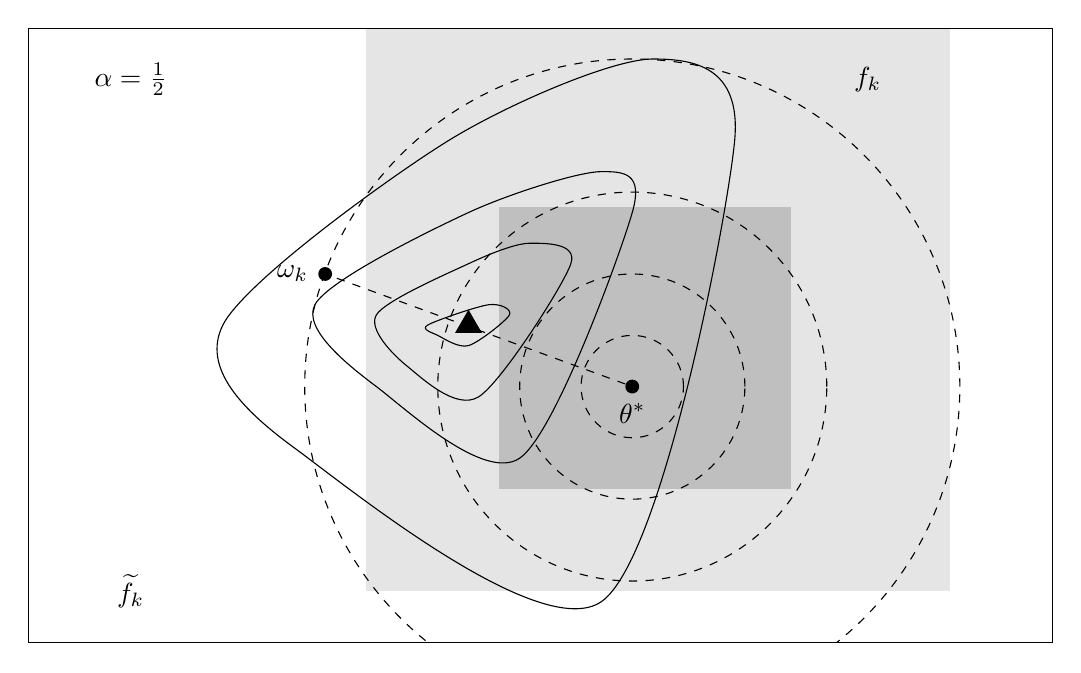
\begin{tikzpicture}[scale=1.3]
% \coordinate (origin) at (0, 0);
\coordinate (rect1) at (-5, -3);
\coordinate (rect2) at (5, 3);
\fill [gray!20] (-1.7, -2.5) rectangle (4, 3);
\fill [gray!50] (-0.4, -1.5) rectangle (2.45, 1.25);
\draw (rect1) rectangle (rect2);
\node at (3.2, 2.5) {$\dom f_k$};
\node at (-4, -2.5) {$\widetilde{\dom f_k}$};
\node at (-4, 2.5) {$\alpha = \frac{1}{2}$};
\draw[] plot [smooth cycle] coordinates {(-1, 0) (-0.7, -0.1) (-0.3, 0.2) (-0.5, 0.3) (-1.1, 0.1)};
\draw[] plot [smooth cycle] coordinates {(-1.3, -0.3) (-0.6, -0.6) (0.3, 0.7) (-0.1, 0.9) (-0.7, 0.7) (-1.6, 0.2)};
\draw[] plot [smooth cycle] coordinates {(-1.6, -0.5) (-0.2, -1.2) (0.9, 1.2) (0.6, 1.6) (-0.7, 1.2) (-2.2, 0.3)};
\draw[] plot [smooth cycle] coordinates {(-2.4, -1.1) (0.6, -2.6) (1.9, 1.9) (1.1, 2.7) (-0.9, 1.9) (-3.1, 0.1)};
\node at (0.9, -0.5) (theta) [circle, fill=black, inner sep=0pt, minimum size=5pt, label=below:{$\theta^*$}] {};
\node at (-2.1, 0.6) (omega1) [circle, fill=black, inner sep=0pt, minimum size=5pt, label=left:{$\omega_k$}] {};
\draw[dashed, thin] (theta) -- (omega1);
\draw plot[only marks, mark=triangle*, mark size=4pt, thick] coordinates {(-0.7, 0.1)};
\begin{scope}
\clip (rect1) rectangle (rect2);
\draw[dashed, thin] (theta) circle (0.5);
\draw[dashed, thin] (theta) circle (1.1);
\draw[dashed, thin] (theta) circle (1.9);
\draw[dashed, thin] (theta) circle (3.2);
\end{scope}
\end{tikzpicture}
\caption{$f_k(\alpha_k \omega_k + (1 - \alpha_k) \theta^*)$的示意图}
\label{fig:apfl}
\end{figure}


\subsection*{动态正则化联邦学习算法\texttt{FedDyn}}
% NOT finished

\parencite{acar2021feddyn}  \texttt{FedDyn}待写。。。。

\begin{algorithm}[ht]
% \SetAlgoNoLine
% \DontPrintSemicolon
\SetKwInOut{Input}{Input}
\Input{penalty coeffecient $\mu$}
{\bfseries Initiation:}\;
\Indp
    {\bfseries Init server:} global model parameters $\theta^{(0)} \in \R^d,$ $h = 0 \in \R^d$\;
    {\bfseries Init clients:} local gradient $\mathfrak{g}_k^{(0)} \gets 0 \in \R^d, ~ \forall k \in [K]$\;
\Indm
\For{each round $t = 0, 1, \cdots, T-1$}{
    $S^{(t)} \gets$ (random set of clients) $\subseteq [K]$\;
    broadcast $\theta^{(t)}$ to clients $k \in S^{(t)}$\;
    \For{each client $k \in \mathcal{S}^{(t)}$ {\bfseries in parallel}}{
        $\theta_k^{(t+1)} \gets \argmin\limits_{\theta_k} \left\{ f_k(\theta_k) - \langle \mathfrak{g}_k^{(t)}, \theta_k \rangle + \frac{\mu}{2} \lVert \theta_k - \theta^{(t)} \rVert^2 \right\}$ \;
        $\mathfrak{g}_k^{(t+1)} \gets \mathfrak{g}_k^{(t)} - \mu (\theta_k^{(t+1)} - \theta^{(t)})$\;
        send $\theta_k^{(t+1)}$ to server\;
    }
    {\bfseries Server Update:}\;
    \Indp
    $h^{(t+1)} \gets h^{(t)} - \frac{1}{\mu} \left(\sum\limits_{k \in S^{(t)}} \theta_k^{(t+1)} - \theta^{(t)} \right)$\;
    $\theta^{(t+1)} \gets \left( \frac{1}{\# S^{(t)}}\sum\limits_{k \in S^{(t)}} \theta_k^{(t+1)} \right) - \frac{1}{\mu} h^{(t+1)}$\;
}
\caption{算法\texttt{FedDyn}\cite{acar2021feddyn}的伪代码}
\label{algo:feddyn}
\end{algorithm}



% \begin{equation}
% \label{eq:fedu}
% \minimize \quad \sum\limits_{k=1}^K f_k(x_k) + \dfrac{\lambda}{2} \sum\limits_{k=1}^K \sum\limits_{j\in\mathcal{N}_k} \lVert \theta_k - \theta_j \rVert^2
% \end{equation}


\subsection*{\texttt{pFedMac}算法}
% NOT finished

\parencite{li2021pfedmac}  \texttt{pFedMac}待写。。。。

\begin{equation}
\label{eq:pfedmac}
\begin{array}{cl}
\minimize & F(\theta) = \frac{1}{K} \sum\limits_{k=1}^K F_i(\theta), \\
\text{where} & F_k(\theta) := \min\limits_{\theta_k} \left\{ f_k(\theta_k) - \mu \langle \theta_k, \theta \rangle + \frac{\mu}{2} \lVert \theta \rVert^2_2 \right\}
\end{array}
\end{equation}

\begin{equation}
\label{eq:pfedmac-sparse}
\begin{array}{cl}
\minimize & F(\theta) = \frac{1}{K} \sum\limits_{k=1}^K F_i(\theta), \\
\text{where} & F_k(\theta) := \min\limits_{\theta_k} \left\{ f_k(\theta_k) - \mu \langle \theta_k, \theta \rangle + \frac{\mu}{2} \lVert \theta \rVert^2_2 + \lVert \theta_k \rVert_1 \right\}
\end{array}
\end{equation}

\begin{algorithm}[ht]
% \SetAlgoNoLine
% \DontPrintSemicolon
\SetKwInOut{Input}{Input}
\Input{learning rate $\eta$, penalty coefficient $\lambda$, $\beta$}
% {\bfseries Server executes:}\;
% \Indp
{\bfseries Initiation:} global (server) model parameters $\theta^{(0)} \in \R^d$\;
\For{each round $t = 0, 1, \cdots, T-1$}{
    $\mathcal{S}^{(t)} \gets$ (random set of clients) $\subseteq [K]$\;
    broadcast $\theta^{(t)}$ to clients $k \in \mathcal{S}^{(t)}$\;
    \For{each client $k \in \mathcal{S}^{(t)}$ {\bfseries in parallel}}{
        $\theta_k^{(t)} \gets$ {\bfseries ClientUpdate}$(k, \theta^{(t)})$\;
        send $\theta_k^{(t)}$ to server\;
    }
    {\bfseries Server Update:}\;
    \Indp
    $\theta^{(t+1)} \gets (1 - \beta) \theta^{(t)} + \frac{\beta}{\lvert \mathcal{S}^{(t)} \rvert} \sum\limits_{k\in \mathcal{S}^{(t)}} \theta_k^{(t)}$\;
    \Indm
}
% \Indm
\vspace{0.2em}
{\bfseries ClientUpdate}$(k, \theta)$: \tcc*[h]{on client $k$}\;
\Indp
$\omega_k^{(t,0)} = \theta_k^{(t,0)} = \theta^{(t)}$\;
\For{local step $r = 0, 1, \cdots, R-1$}{
    $\mathcal{D}_{k, r} \gets$ (sample a mini-batch data)\;
    $\omega_k^{(t,r)} \gets \argmin_{\omega_k} \left\{ \ell_k(\omega_k; \mathcal{D}_{k, r}) - \lambda \langle \omega_k, \theta_k^{(t,r)} \rangle \right\}$\;
    $\theta_k^{(t,r+1)} \gets \theta_k^{(t,r)} - \eta\lambda \left( \theta_k^{(t,r)} - \omega_k^{(t,r)} \right)$\;
}
\Return{$\theta_k^{(t,R)}$}
\caption{算法\texttt{pFedMac}\cite{li2021pfedmac}的伪代码}
\label{algo:pfedmac}
\end{algorithm}


待写。。。。


%\mbox{}\newpage
\chapter{\hspace{-1mm}\bf 个性化联邦学习中的算子分裂算法}
\label{chap4}
\addcontentsline{toe}{chapter}{{{\bf Chapter \currentchapter \ 
Operator Splitting Algorithms for Personalized Federated Learning }}\numberline\,}
\markboth{第 \currentchapter \ 章\ \ 
个性化联邦学习中的算子分裂算法}{北京航空航天大学博士后研究工作报告}

%%%%%%%%%%%%%%%%%%%%%%%%%%%%%%%%%%%%%%%%%%%%%%%%%%%%%%%%%%%


\section{个性化联邦学习问题建模}
\addcontentsline{toe}{section}{{4.1\ \ Problem Formulation for Personalized Federated Learning}\numberline\,}
\label{sec:chap4-prob-form}

% NOT finished
% NOT indexed

待写 。。。。


\section{个性化联邦学习的算子分裂法}
\addcontentsline{toe}{section}{{\thesection\ \ Novel Operator Splitting Algorithm for Personalized Federated Learning}\numberline\,}
\label{sec:chap4-pfl-os-algo}

% NOT finished
% NOT indexed

待写 。。。。

% \cite{Han_2013_CDRSM}



\printbibliography[title=参考文献]

\backmatter
\chapter*{博士后在站期间的主要成果}
\addcontentsline{toc}{chapter}{{博士后在站期间的主要成果}\numberline~~~}
\addcontentsline{toe}{chapter}{{Main achievements during the postdoctoral program}\numberline ~~~}
\markboth{博士后在站期间的主要成果}{博士后在站期间的主要成果}\headheight=15.24pt%5mm

\noindent{\larger \heiti 基金项目:}

\begin{itemize}
    \item 面向脊柱穿刺消融手术的多模态图像导航关键算法研究,数学天元基金项目/数学天元基金/数学与医疗健康交叉重点专项,参与,起止时间:2022/01 -- 2023/12。
    \item 数字电路物理设计自动化中关键数学问题研究,国家重点研发计划,参与,起止时间:2022/05 -- 2025/04。
\end{itemize}

\noindent{\larger \heiti 科研论文:}

\begin{enumerate}
    \item WEN H, KANG J. Hybrid Arrhythmia Detection on Varying-Dimensional Electrocardiography: Combining Deep Neural Networks and Clinical Rules[C]//2021 Computing in Cardiology (CinC): vol. 48. Institute of Electrical and Electronics Engineers (IEEE), 2021. DOI: 10.23919/cinc53138.2021.9662801.
    \item KANG J, WEN H. A Study on Several Critical Problems on Arrhythmia Detection using Varying-Dimensional Electrocardiography[J]. Physiological Measurement, 2022, 43(6): 064007. DOI: 10.1088/1361-6579/ac6aa3.
    \item WEN H, KANG J. A Novel Deep Learning Package for Electrocardiography Research[J]. Physiological Measurement, 2022, 43(11): 115006. DOI: 10.1088/1361-6579/ac9451.
    \item WEN H, KANG J. A Comparative Study on Neural Networks for Paroxysmal Atrial Fibrillation Events Detection from Electrocardiography[J]. Journal of Electrocardiology, 2022, 75: 19-27. DOI: 10.1016/j.jelectrocard.2022.10.002.
    \item GU E, CHEN Y, WEN H, CAI X, HAN D. Novel Clustered Federated Learning Based on Local Loss. 2023. Submitted.
\end{enumerate}

% \patchcmd{\thebibliography}{\section*}{\chapter*}{}{}

% \begin{refsection}[publications.bib]
% \nocite{wen_cinc2021, Kang_2022_cinc2021_iop, torch_ecg_paper, Wen_cpsc2021, wen_cinc2022}
% \printbibliography[title={\heiti 科研论文}]
% \end{refsection}


\chapter*{致~~~谢}\vskip1cm
\addcontentsline{toc}{chapter}{{致谢}\numberline ~~~}
\addcontentsline{toe}{chapter}{{Acknowledgement}\numberline ~~~}
\markboth{致~~~谢}{北京航空航天大学博士后研究工作报告}
\vspace{-1.0cm}

% finished

首先,我衷心感谢我合作导师韩德仁教授,感谢他将联邦学习这一国际前沿的研究领域介绍给我,以他的博学多识以及敏锐的直觉,给我指引研究的方向,对相关的难点问题对我进行悉心的指导,使我受益匪浅。

我要感谢北京航空航天大学数学科学学院统计与运筹系以及计算科学系的老师以及同学们:崔春风、谢家新、邓钊、于冬梅、黄博、靳正芬、陈彩荣、路宁、顾恩东、屈云飞、陈鑫、陈永鑫、王青松、胡乐宇、苏宴生、刘锐、苌远等,以及南京师范大学的蔡邢菊教授,协助我组织联邦学习讨论班,积极参与问题的讨论,在我的研究过程中给了我很多有益的建议,对我的帮助极大。

我要感谢北京航空航天大学数学科学学院的行政机关的老师们:齐丹、陆筱、赵丽君、鲁琛、曹安妮、李田田、徐田梅,他们出色而专业的工作,保障了我科研工作的顺利进行。

我还要感谢我的父母,我的妻子,我的岳母还有我的女儿,给我鼓励与支持,让我没有后顾之忧,让我能够全情投入于博士后课题的研究。

\vspace{-2cm}
\textit{ \vskip 1in \centerline{{\mbox{}\hskip 13cm}文豪}
\vskip 0in
\centerline{{\mbox{}\hskip 12.3cm}2023\,年\,6\,月}
}


\end{document}
